%\documentclass[a4paper,landscape, 5pt]{article}
\documentclass[10pt]{article}
\usepackage[a4paper, margin=0.1in, landscape]{geometry}
%\usepackage{graphicx} % Required for inserting images
\usepackage{graphicx}
\usepackage{multicol}
\usepackage{xcolor}
\usepackage{amsfonts}
\usepackage{wrapfig}
\usepackage{amsmath}  % For various math symbols and 
\usepackage{amssymb}  % For additional math symbols
\usepackage{mathrsfs}
\usepackage{bm}       % For bold math symbols

\usepackage{lipsum}

\usepackage[compact]{titlesec}
% Change title spacing
\titlespacing{\section}{0pt}{*0}{*0}
\titlespacing{\subsection}{0pt}{*0}{*0}
\titlespacing{\subsubsection}{0pt}{*0}{*0}

% Change title color
% \newcommand{\sectionnewcolor}[1]{%
%     \definecolor{section_color}{rgb}{#1}%
%     \titleformat*{\section}{\normalfont\normalsize\bfseries\color{section_color}}%
%     \titleformat*{\subsection}{\normalfont\normalsize\bfseries\color{section_color}}%
%     \titleformat*{\subsubsection}{\normalfont\normalsize\bfseries\color{section_color}}%
% }
\definecolor{default_section_color}{rgb}{0,0,0} % Default color

\definecolor{color1}{rgb}{0.8,0.2,0.2}   % Red
\definecolor{color2}{rgb}{0.2,0.2,0.8}   % Blue
\definecolor{color3}{rgb}{0.2,0.6,0.6}   % Cyan
\definecolor{color4}{rgb}{0.8,0,0.8}     % Magenta
\definecolor{color5}{rgb}{1,0.5,0}        % Orange
\definecolor{color6}{rgb}{0.5,0,0.5}      % Purple
\definecolor{color7}{rgb}{0,0.5,0.5}      % Teal
\definecolor{color8}{rgb}{0.6,0.3,0.1}    % Brown
\definecolor{color9}{rgb}{0.4,0.4,0.4}    % Dark Gray
\definecolor{color10}{rgb}{0,0.8,0}       % Green
% \definecolor{color11}{rgb}{0.8,0.8,0}     % Yellow
\definecolor{color12}{rgb}{0,0.7,0.7}     % Sky Blue
\definecolor{color13}{rgb}{0.7,0,0.7}     % Violet
\definecolor{color14}{rgb}{0.7,0.7,0}     % Olive
\definecolor{color15}{rgb}{0.4,0,0}       % Maroon
\definecolor{color16}{rgb}{0.5,0.5,0.1}   % Olive Drab
\definecolor{color17}{rgb}{0.5,0,0.2}     % Dark Brown
\definecolor{color18}{rgb}{0,0.4,0.2}     % Forest Green
\definecolor{color19}{rgb}{0.6,0.4,0.2}   % Sienna
\definecolor{color20}{rgb}{0.3,0.7,0.7}   % Light Blue
\definecolor{color21}{rgb}{0.8,0.6,0.1}   % Gold
\definecolor{color22}{rgb}{0.7,0.4,0.4}   % Indian Red
\definecolor{color23}{rgb}{0.2,0.8,0.2}   % Lime Green
\definecolor{color24}{rgb}{0.8,0.4,0.7}   % Pink
\definecolor{color25}{rgb}{0.5,0.5,0.8}   % Light Slate Blue
\definecolor{color26}{rgb}{0.5,0.7,0.3}   % Medium Sea Green
\definecolor{color27}{rgb}{0.4,0.8,0.6}   % Medium Aquamarine
\definecolor{color28}{rgb}{0.3,0.3,0.7}   % Medium Slate Blue
\definecolor{color29}{rgb}{0.8,0.3,0.6}   % Medium Purple
\definecolor{color30}{rgb}{0.4,0.4,0.8}   % Slate Blue
\newcounter{colornumber}
\setcounter{colornumber}{0}
\newcommand{\sectionnewcolor}{%
    \ifcase\thecolornumber%
        \colorlet{section_color}{color1}%
    \or
        \colorlet{section_color}{color2}%
    \or
        \colorlet{section_color}{color3}%
    \or
        \colorlet{section_color}{color4}%
    \or
        \colorlet{section_color}{color5}%
    \or
        \colorlet{section_color}{color6}%
    \or
        \colorlet{section_color}{color7}%
    \or
        \colorlet{section_color}{color8}%
    \or
        \colorlet{section_color}{color9}%
    \or
        \colorlet{section_color}{color10}%
    % \or
    %     \colorlet{section_color}{color11}%
    \or
        \colorlet{section_color}{color12}%
    \or
        \colorlet{section_color}{color13}%
    \or
        \colorlet{section_color}{color14}%
    \or
        \colorlet{section_color}{color15}%
    \or
        \colorlet{section_color}{color16}%
    \or
        \colorlet{section_color}{color17}%
    \or
        \colorlet{section_color}{color18}%
    \or
        \colorlet{section_color}{color19}%
    \or
        \colorlet{section_color}{color20}%
    \or
        \colorlet{section_color}{color21}%
    \or
        \colorlet{section_color}{color22}%
    \or
        \colorlet{section_color}{color23}%
    \or
        \colorlet{section_color}{color24}%
    \or
        \colorlet{section_color}{color25}%
    \or
        \colorlet{section_color}{color26}%
    \or
        \colorlet{section_color}{color27}%
    \or
        \colorlet{section_color}{color28}%
    \or
        \colorlet{section_color}{color29}%
    \or
        \colorlet{section_color}{color30}%
    \else
        \colorlet{section_color}{default_section_color}%
    \fi
    
    \titleformat*{\section}{\normalfont\normalsize\bfseries\color{section_color}}%
    \titleformat*{\subsection}{\normalfont\normalsize\bfseries\color{section_color}}%
    \titleformat*{\subsubsection}{\normalfont\normalsize\bfseries\color{section_color}}%
    \stepcounter{colornumber}%
}


\newcommand{\sectiondivider}{%
    \vspace{4pt}%
    \hrule%
    \vspace{4pt}%
}

% Change text spacing
\setlength{\parindent}{0pt}
\setlength{\columnseprule}{0.2pt}
\setlength{\intextsep}{0pt}%
% \setlength{\columnsep}{7pt}%

\usepackage{enumitem} % To remove indent of enumerate
\setlist[enumerate]{wide, topsep=0pt,itemsep=0pt,partopsep=0pt, parsep=0pt, labelwidth=!, labelindent=0pt}

\setlist[itemize]{wide, topsep=0pt,itemsep=0pt,partopsep=0pt, parsep=0pt, labelwidth=!, labelindent=0pt}

\usepackage{manfnt} % for writing a cube: \mbox{\mancube}


\begin{document}

\begin{multicols*}{4}

\sectionnewcolor
\section*{Regression}
\subsection*{Terminology}

- Data consists of \textbf{pairs} ($\mathbf{x}_n$, $y_n$), where $y_n$ is the n’th output and $x_n$ is a vector of $D$ inputs. The number of pairs $N$ is the data-size and $D$ is the dimensionality.

- Two goals of regression: \textbf{prediction} and \textbf{interpretation}

- The regression function: $y_{n}\approx f_w(\mathbf{x}_{n})\ \forall n$

- Regression finds correlation not a causal relationship.

- \textbf{Input variables} a.k.a. covariates, independent variables, explanatory variables, exogenous variables, predictors, regressors. 

- \textbf{Output variables} a.k.a. target, label, response, outcome, dependent variable, endogenous variables, measured variable, regressands.

\subsection*{Linear Regression}

- Assumes linear relationship between inputs and output.

- $y_{n}\approx\,f(\mathbf{x}_{n}) :=w_{0}+w_{1}x_{n1}+ ... +w_{D}x_{n D} \\ := \tilde{\bf x}_{n}^{T} \tilde{\bf w}$ contain the additional offset term (\small{a.k.a. bias}).

- Given data we learn the weights $\mathbf{w}$ (\small{a.k.a. estimate or fit the model})

- Overparameterisation $D > N$ eg. univariate linear regression with a single data point $y_{1}\approx w_{0}+w_{1}x_{11}$. This makes the task under-determined (no unique solution).

\subsection*{Loss Functions $\mathcal{L}$}

- A loss function (a.k.a. energy, cost, training objective) quantifies how well the model does (how costly its mistakes are).

- $y \in \mathbb{R} \Rightarrow$ desirable for cost to be symmetric around 0 since $\pm$ errors should be penalized equally.

- Cost function should penalize “large” mistakes and “very large” mistakes similarly to be robust to outliars.

- Mean Squared Error: \\ ${\mathsf{MSE}}(\mathbf{w}):={\frac{1}{N}}\sum_{n=1}^{N}\left[y_{n}-f_{\mathrm{w}}(\mathbf{x}_{n})\right]^{2}$ \\ not robust to outliars.

- Mean Absolute Error: \\ ${\mathsf{MAE}}(\mathbf{w}):={\frac{1}{N}}\sum_{n=1}^{N}|y_{n}-f_{\mathrm{w}}(\mathbf{x}_{n})|$

- Convexity: a function is convex iff a line segment between two points on the function’s graph always lies above the function.

- Convexity: a function $h(\mathbf{u}), \mathbf{u} \in \mathbb{R}^D$ is convex if $\forall \ \mathbf{u}, \mathbf{v} \in \mathbb{R}^D, 0 \leq \lambda \leq  1$: \\ $h(\lambda\mathbf{u}+(1-\lambda)\mathbf{v}) \ \textcolor[RGB]{255,0,0}{\leq} \ \lambda h(\mathbf{u})+(1-\lambda)h(\mathbf{v})$ \\Stirctly convex if $\textcolor[RGB]{255,0,0}{\leq} \Rightarrow \textcolor[RGB]{255,0,0}{<}$ 

- Convexity, a desired computational property:
A strictly convex function has a unique global minimum $\mathbf{w^{*}}$. For convex functions, every local minimum is a global minimum.

- Sums of convex functions are also convex $\Rightarrow$ MSE combined with a linear model is convex in $\mathbf{w}$.

- Proof of convexity for MAE:

\scalebox{0.7}{
$\begin{array}{l}
    {\mathsf{MAE}(\mathbf{w}) := \frac{1}{N} \sum_{n=1}^{N} \mathcal{L}_n(\mathbf{w}), \mathcal{L}_n(\mathbf{w})=|y_{n}-f_{\mathrm{w}}(\mathbf{x}_{n})|} 
    \\ 
    {\mathcal{L}_n(\lambda w_1 + (1-\lambda)w_2) \leq \lambda \mathcal{L}_n(w_1)+(1-\lambda)\mathcal{L}_n(w_2)} 
    \\ 
    {| y_n-x_n^{T}(\lambda w_1 + (1-\lambda)w_2)| \leq \lambda |{y_n-x_n^{T}w_1}| + (1-\lambda)|{y_n-x_n^{T}w_2}|}
    \\
    {(1-\lambda) \geq 0 \Rightarrow (1-\lambda)|{y_n-x_n^{T}w_2}|=|(1-\lambda)y_{n}-(1-\lambda)x_{n}^{T}w_2|}
    \\
    {a=\lambda y_{n}-\lambda x_{n}^{T}w_{1}, b=(1-\lambda)y_{n}-(1-\lambda)x_{n}^{T}w_{2}}
    \\
    {a+b=y_{n}-x_{n}^{T}(\lambda w_{1}+(1-\lambda)w_{2})}
    \\
    {|a + b| \leq |a| + |b| \Rightarrow \mathcal{L}_n(\mathbf{w}) \ \mathsf{convex}\Rightarrow \mathsf{MAE}(\mathbf{w}) \ \mathsf{convex}}
\end{array}$
}

- Huber loss: \\
${\cal H}u b e r(e):=\left\{\begin{array}{l l}{{\frac{1}{2}e^{2}}}&{{,\mathrm{if}\ |e|\leq\delta}}\\ {{\delta|e|-\frac{1}{2}\delta^{2}}}&{{,\mathrm{if}\ |e|>\delta}}\end{array}\right.$ convex, differentiable, and robust to outliers but setting $\delta$ is not easy.

- Tukey’s bisquare loss: \\
$\frac{\partial\mathcal{L}}{\partial e}:=\left\{\begin{array}{l l}{{e\{1-e^{2}/\delta^{2}\}^{2}}}&{{,\mathrm{if}\,\,|e|\leq\delta}}\\ {{0}}&{{,\mathrm{if} \ |e| > \delta}}\end{array}\right.$ non-convex, but robust to outliers.

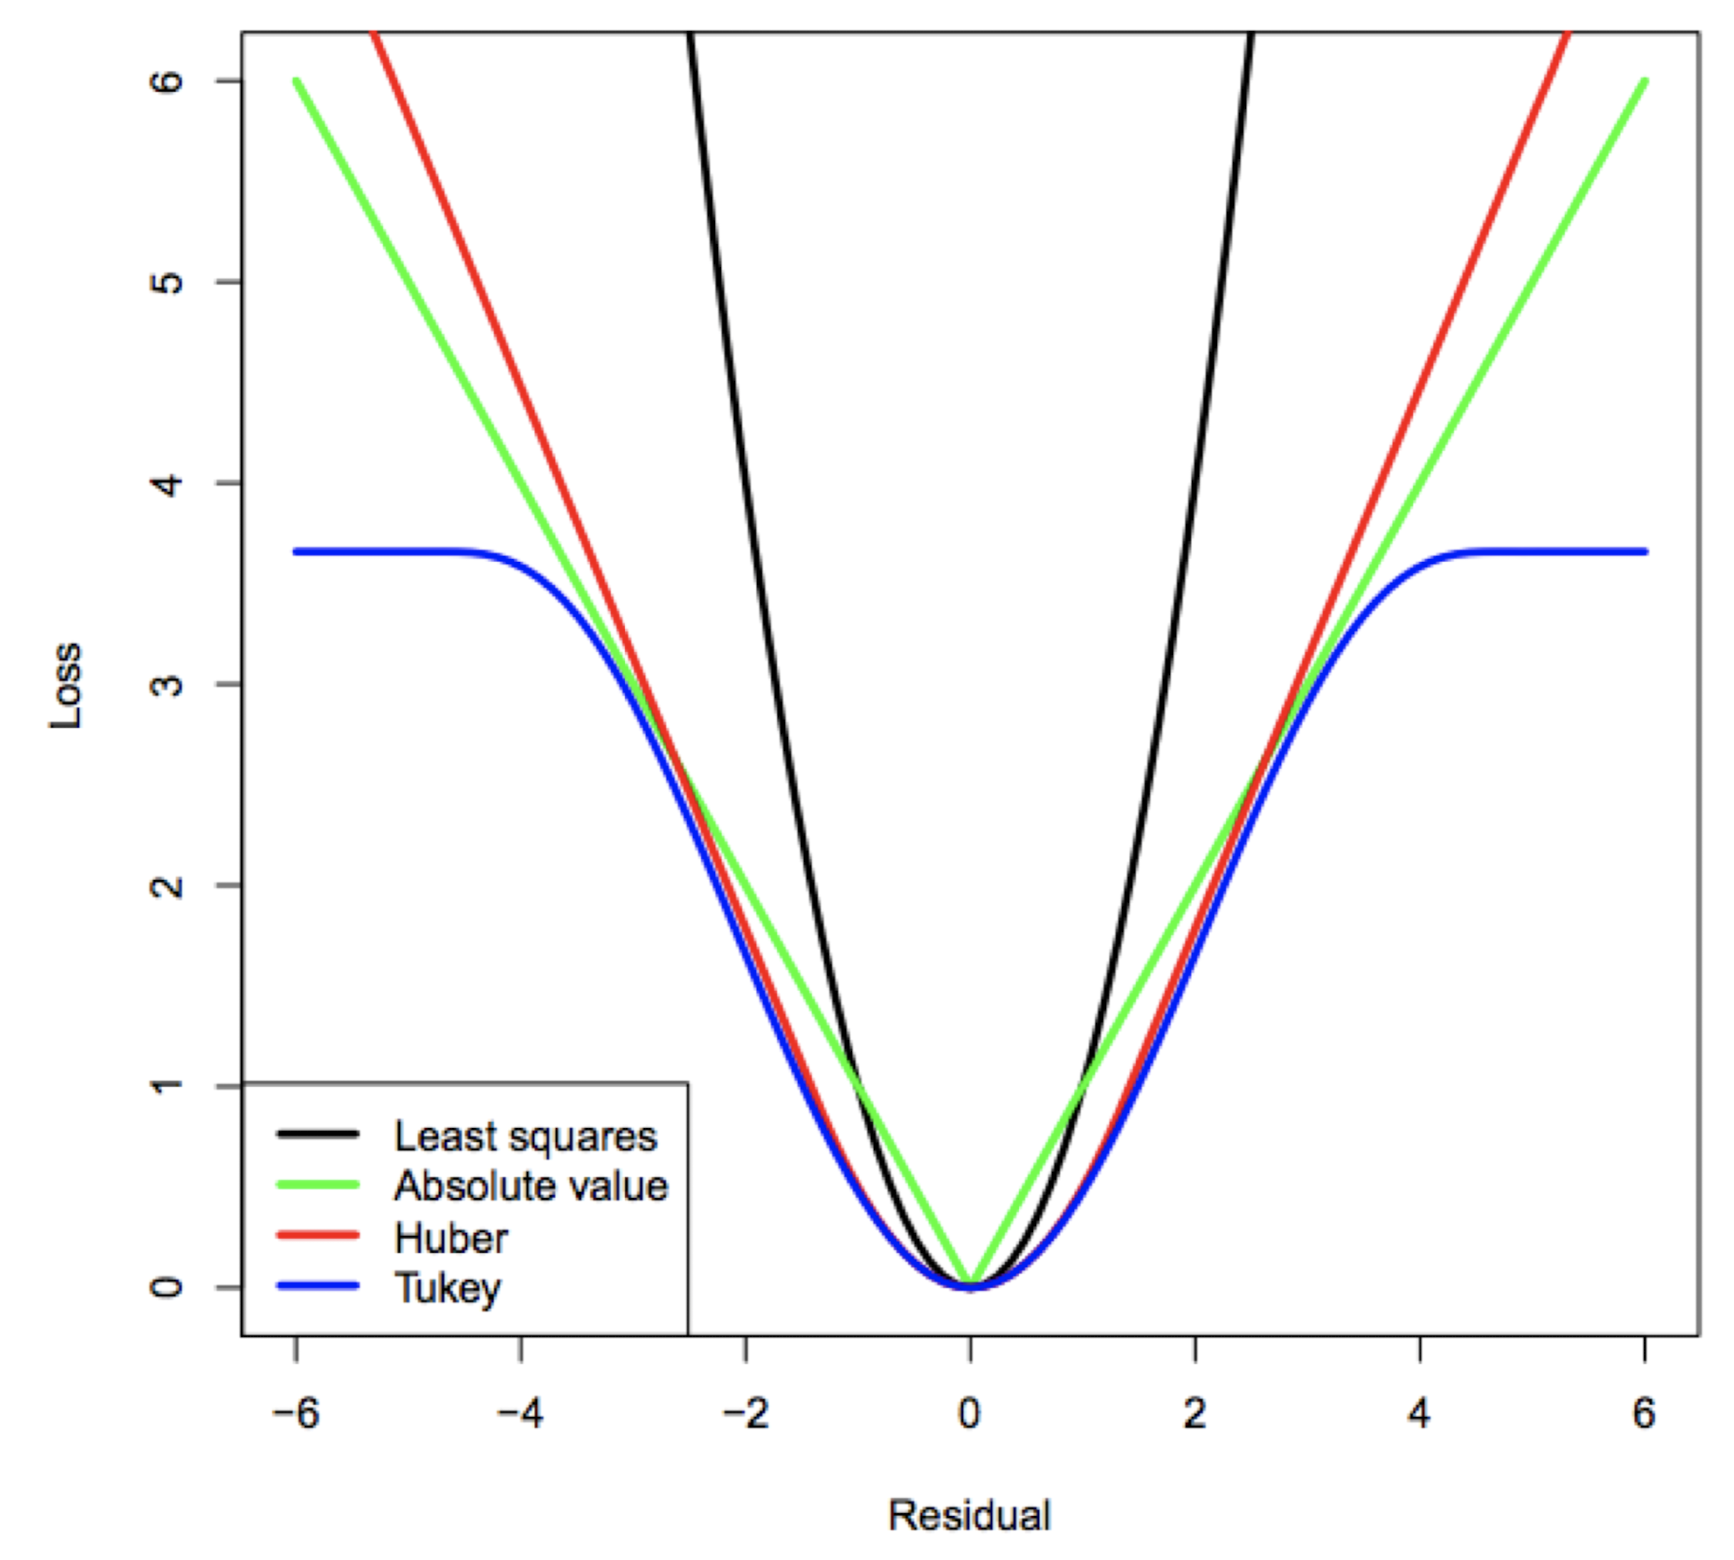
\includegraphics[width=\linewidth]{loss_functions.png}
\sectiondivider

\sectionnewcolor
\section{Optimisation}

- Given $\mathcal{L}(\mathbf{w})$ we want $\mathbf{w^*} \in \mathbb{R}^D$ which minimises the cost: $\min_\mathbf{w} \mathcal{L}(\mathbf{w}) \rightarrow$ formulated as an optimisation problem

- Local minimum $\mathbf{w^*} \Rightarrow \exists \epsilon > 0$ s.t. \\
$\mathcal{L}(\mathbf{w^*}) \leq \mathcal{L}(\mathbf{w}) \ \forall \mathbf{w} \ \mathrm{with} \ \Vert \mathbf{w}-\mathbf{w^*} \Vert < \epsilon$

- Global minimum $\mathbf{w^*}$,
$\mathcal{L}(\mathbf{w^*}) \leq \mathcal{L}(\mathbf{w}) \ \forall \mathbf{w} \in \mathbb{R}^D$

\subsection{Smooth Optimisation}

\vspace{4pt}
\hrule
\vspace{4pt}
\sectiondivider

\sectionnewcolor

\section*{Least Squares}
- Linear regression + MSE $\rightarrow$ compute the optimum of the cost function analytically by solving a linear system of $D$ equations (normal equations)

- Derive the normal equations, proove convexity, optimality conditions for convex functions ($
\nabla \mathcal{L}\left(\mathbf{w}^{\star}\right)=\mathbf{0} .
$)

\subsection*{Normal Equations}
$\mathcal{L}(\mathbf{w})=\frac{1}{2 N} \sum_{n=1}^{N}\left(y_{n}-\mathbf{x}_{n}^{\top} \mathbf{w}\right)^{2}\\=\frac{1}{2 N}(\mathbf{y}-\mathbf{X} \mathbf{w})^{\top}(\mathbf{y}-\mathbf{X} \mathbf{w})$,

% where

% $\mathbf{y}=\left[\begin{array}{c}y_{1} \\ y_{2} \\ \vdots \\ y_{N}\end{array}\right], \mathbf{X}=\left[\begin{array}{cccc}x_{11} & x_{12} & \ldots & x_{1 D} \\ x_{21} & x_{22} & \ldots & x_{2 D} \\ \vdots & \vdots & \ddots & \vdots \\ x_{N 1} & x_{N 2} & \ldots & x_{N D}\end{array}\right]$

- Proof of convexity:

1) Simplest way: observe that $\mathcal{L}$ is naturally represented as the sum (with positive coefficients) of the simple terms $\left(y_{n}-\mathbf{x}_{n}^{\top} \mathbf{w}\right)^{2}$. Further, each of these simple terms is the composition of a linear function with a convex function (the square function). Therefore, each of these simple terms is convex and hence the sum is convex.

2) Directly verify the definition, that for any $\lambda \in[0,1]$ and $\mathbf{w}, \mathbf{w}^{\prime}$

\text{\footnotesize
$\mathcal{L}\left(\lambda \mathbf{w}+(1-\lambda) \mathbf{w}^{\prime}\right)-\left(\lambda \mathcal{L}(\mathbf{w})+(1-\lambda) \mathcal{L}\left(\mathbf{w}^{\prime}\right)\right) \leq 0$.
}

$\mathrm{LHS}=$
$-\frac{1}{2 N} \lambda(1-\lambda)\left\|\mathbf{X}\left(\mathbf{w}-\mathbf{w}^{\prime}\right)\right\|_{2}^{2} < 0$,


3) We can compute the second derivative (the Hessian) and show that it is positive semidefinite (all its eigenvalues are non-negative). 

$\begin{aligned}
    \mathbf{H}(\mathbf{w})& =\frac{1}{2N}\nabla^2\left(\left(\mathbf{y}-\mathbf{X}\mathbf{w}\right)^\top\left(\mathbf{y}-\mathbf{X}\mathbf{w}\right)\right)  \\
    &=\frac{1}{2N}\nabla\left(-2(\mathbf{y}-\mathbf{X}\mathbf{w})\mathbf{X}^\top\right) \\
    &=\frac{-2}{2N}\nabla(\mathbf{X}^\top(\mathbf{y}-\mathbf{X}\mathbf{w})) \\
    &=\frac{-1}N\mathbf{X}^\top\nabla(\mathbf{y}-\mathbf{X}\mathbf{w}) \\
    &=\frac{-1}N\mathbf{X}^\top(\nabla\mathbf{y}-\nabla(\mathbf{X}\mathbf{w})) \\
    &=\frac{-1}N\mathbf{X}^\top(\mathbf{0}-\mathbf{X}) \\
    &=\frac1N\mathbf{X}^\top\mathbf{X}
\end{aligned}$

Singular value decomposition (SVD):
$
\mathbf{X}=\mathbf{US}\mathbf{V}^\top 
$
U and V are orthogonal matrices, and S is a diagonal matrix with the singular values $\sigma_i$ on the diagonal.

$
\mathbf{H}(\mathbf{w})=\frac1N\mathbf{X}^\top\mathbf{X}=\frac1N\mathbf{V}\mathbf{S}^2\mathbf{V}^\top 
$

where $\mathbf{S}^2$ is a diagonal matrix with the squares of the singular values. 

Let $\mathbf{v}$ be a non-zero vector,

$
\begin{aligned}
\mathbf{v}^\top\mathbf{H}(\mathbf{w})\mathbf{v}& =\frac1N\mathbf{v}^\top\mathbf{V}\mathbf{S}^2\mathbf{V}^\top\mathbf{v} \\
&=\frac1N(\mathbf{V}^\top\mathbf{v})^\top\mathbf{S}^2(\mathbf{V}^\top\mathbf{v}) \\
&=\frac1N\|\mathbf{S}(\mathbf{V}^\top\mathbf{v})\|^2 \geq 0
\end{aligned}
$

$\mathbf{S}$ diagonal matrix with non-negative entries, $\mathbf{V}^\top\mathbf{v}$ vector.


- Now find its minimum

$
\nabla \mathcal{L}(\mathbf{w})=-\frac{1}{N} \mathbf{X}^{\top}(\mathbf{y}-\mathbf{X} \mathbf{w}) = \mathbf{0}\\
\Rightarrow\mathbf{X}^{\top} \underbrace{(\mathbf{y}-\mathbf{X} \mathbf{w})}_{\text {error }}=\mathbf{0}
$

\subsection*{Geometric Interpretation}

% \begin{center}
    \includegraphics*[width=0.7\columnwidth]{figures/geom_ls.png}
% \end{center}


\subsection*{Closed form}
- $\mathbf{X}^{\top} \mathbf{X} \in \mathbb{R}^{D \times D}$ is called the Gram matrix. 

- If invertible, we can get a closed-form expression for the minimum:

$
\mathbf{w}^{\star}=\left(\mathbf{X}^{\top} \mathbf{X}\right)^{-1} \mathbf{X}^{\top} \mathbf{y}
$

\subsection*{Invertibility and Uniqueness}
- $\mathbf{X}^{\top} \mathbf{X} \in \mathbb{R}^{D \times D}$ invertible iff $\operatorname{rank}(\mathbf{X})=D$.

- Proof: assume $\operatorname{rank}(\mathbf{X})<D$. Then there exists a non-zero vector $\mathbf{u}$ so that $\mathbf{X u}=\mathbf{0}$. It follows that $\mathbf{X}^{\top} \mathbf{X u}=\mathbf{0}$, and so $\operatorname{rank}\left(\mathbf{X}^{\top} \mathbf{X}\right)<D$. Therefore, $\mathbf{X}^{\top} \mathbf{X}$ is not invertible.

Conversely, assume that $\mathbf{X}^{\top} \mathbf{X}$ is not invertible. Hence, there exists a non-zero vector $\mathbf{v}$ so that $\mathbf{X}^{\top} \mathbf{X v}=\mathbf{0}$. It follows that

$$
\mathbf{0}=\mathbf{v}^{\top} \mathbf{X}^{\top} \mathbf{X} \mathbf{v}=(\mathbf{X} \mathbf{v})^{\top}(\mathbf{X} \mathbf{v})=\|\mathbf{X} \mathbf{v}\|^{2}
$$

This implies that $\mathbf{X v}=\mathbf{0}$, i.e., $\operatorname{rank}(\mathbf{X})<D$.

\subsection*{Rank Deficiency and Ill-Conditioning}
- In practice, $\mathbf{X}$ is often rank deficient.

- If $D>N$, we always have $\operatorname{rank}(\mathbf{X})<D$ (since row rank $=$ col. rank)

- If $D \leq N$, but some of the columns $\mathbf{x}_{:}$are (nearly) collinear, then the matrix is illconditioned, leading to numerical issues when solving the linear system.

- Using a linear system solver, one can solve this problem.

\subsection*{Closed-form solution for MAE}
Can you derive closed-form solution for 1-parameter model when using MAE cost function?


\sectiondivider

\sectionnewcolor
\section{Maximum Likelihood}

\subsection*{Gaussian distribution and independence}
% - A Gaussian random variable in $\mathbb{R}$ with mean $\mu$ and variance $\sigma^{2}$ has a density of

$p(y \mid \mu, \sigma^{2})=\mathcal{N}(y \mid \mu, \sigma^{2})=\frac{1}{\sqrt{2 \pi \sigma^{2}}} \exp [-\frac{(y-\mu)^{2}}{2 \sigma^{2}}]$,
$\boldsymbol{\Sigma}$ psd.

$\mathcal{N}(\mathbf{y} \mid \boldsymbol{\mu}, \boldsymbol{\Sigma})=\frac{1}{\sqrt{(2 \pi)^{D} \operatorname{det}(\boldsymbol{\Sigma})}} \exp [-\frac{1}{2}(\mathbf{y}-\boldsymbol{\mu})^{\top} \boldsymbol{\Sigma}^{-1}(\mathbf{y}-\boldsymbol{\mu})]$

- Two RVs $X$, $Y$ independent when $p(x, y)=p(x) p(y)$.

\subsection*{A probabilistic model for least-squares}

- $
y_{n}=\mathbf{x}_{n}^{\top} \mathbf{w}+\epsilon_{n}
$ where the $\epsilon_{n}$ zero mean Gaussian RV

% - Given $N$ samples, the likelihood of the data vector $\mathbf{y}=$ $(y_{1}, \cdots, y_{N})$ given the input $\mathbf{X}$ and the model $\mathbf{w}$ is equal to

$p(\mathbf{y} \mid \mathbf{X}, \mathbf{w})=\prod_{n=1}^{N} p(y_{n} \mid \mathbf{x}_{n}, \mathbf{w})=\prod_{n=1}^{N} \mathcal{N}(y_{n} \mid \mathbf{x}_{n}^{\top} \mathbf{w}, \sigma^{2})$

% - Maximize this likelihood over the choice of model w.

\subsection*{Defining cost with log-likelihood}

$\mathcal{L}_{\mathrm{LL}}(\mathbf{w}):=\log p(\mathbf{y} \mid \mathbf{X}, \mathbf{w})=-\frac{1}{2 \sigma^{2}} \sum_{n=1}^{N}(y_{n}-\mathbf{x}_{n}^{\top} \mathbf{w})^{2}+$ cnst.

\subsection*{Maximum-likelihood estimator (MLE)}

$\arg \min _{\mathbf{w}} \mathcal{L}_{\mathrm{MSE}}(\mathbf{w})=\arg \max _{\mathbf{w}} \mathcal{L}_{\mathrm{LL}}(\mathbf{w})$.

% - MLE $\rightarrow$ finding the model under which the observed data is most likely to have been generated from (probabilistically).

\subsection*{Properties of MLE}
- MLE is a sample approximation to the expected log-likelihood:
$
\mathcal{L}_{\mathrm{LL}}(\mathbf{w}) \approx \mathbb{E}_{p(y, \mathbf{x})}[\log p(y \mid \mathbf{x}, \mathbf{w})]
$

- MLE is consistent, i.e., it will give us the correct model assuming that we have a sufficient amount of data.
$\mathbf{w}_{\text {MLE }} \longrightarrow^{p} \mathbf{w}_{\text {true }}$

- The MLE is asymptotically normal, i.e.,

$(\mathbf{w}_{\text {MLE }}-\mathbf{w}_{\text {true }}) \longrightarrow^{d} \frac{1}{\sqrt{N}} \mathcal{N}(\mathbf{w}_{\text {MLE }} \mid \mathbf{0}, \mathbf{F}^{-1}(\mathbf{w}_{\text {true }}))$

where $\mathbf{F}(\mathbf{w})=-\mathbb{E}_{p(\mathbf{y})}[\frac{\partial^{2} \mathcal{L}}{\partial \mathbf{w} \partial \mathbf{w}^{\top}}]$ is the Fisher information.

- MLE is efficient, i.e. it achieves the Cramer-Rao lower bound. Covariance $(\mathbf{w}_{\text {MLE }})=\mathbf{F}^{-1}(\mathbf{w}_{\text {true }})$

\subsection*{Laplace distribution $
p(y_{n} \mid \mathbf{x}_{n}, \mathbf{w})=\frac{1}{2 b} e^{-\frac{1}{b}|y_{n}-\mathbf{x}_{n}^{\top} \mathbf{w}|}
$}


\sectiondivider

\sectionnewcolor

\section*{Regularization}
We have seen that by augmenting the feature vector we can make linear models as powerful as we want. Unfortunately this leads to the problem of overfitting. Regularization is a way to mitigate this undesirable behavior.

We will discuss regularization in the context of linear models, but the same principle applies also to more complex models such as neural nets.

\section*{Regularization}
Through regularization, we can penalize complex models and favor simpler ones:

$$
\min _{\mathbf{w}} \mathcal{L}(\mathbf{w})+\Omega(\mathbf{w})
$$

The second term $\Omega$ is a regularizer, measuring the complexity of the model given by $\mathbf{w}$.

\section*{$L_{2}$-Regularization: Ridge Regression}
The most frequently used regularizer is the standard Euclidean norm $\left(L_{2^{-}}\right.$ norm), that is

$$
\Omega(\mathbf{w})=\lambda\|\mathbf{w}\|_{2}^{2}
$$

where $\|\mathbf{w}\|_{2}^{2}=\sum_{i} w_{i}^{2}$. Here the main effect is that large model weights $w_{i}$ will be penalized (avoided), since we consider them "unlikely", while small ones are ok. When $\mathcal{L}$ is MSE, this is called ridge regression:

$\min _{\mathbf{w}} \frac{1}{2 N} \sum_{n=1}^{N}\left[y_{n}-\mathbf{x}_{n}^{\top} \mathbf{w}\right]^{2}+\lambda\|\mathbf{w}\|_{2}^{2}$

Least squares is a special case of this: set $\lambda:=0$.

\section*{Explicit solution for w: Differ-}
entiating and setting to zero:

$$
\mathbf{w}_{\text {ridge }}^{\star}=\left(\mathbf{X}^{\top} \mathbf{X}+\lambda^{\prime} \mathbf{I}\right)^{-1} \mathbf{X}^{\top} \mathbf{y}
$$

(here for simpler notation $\frac{\lambda^{\prime}}{2 N}=\lambda$ )

\section*{Ridge Regression to Fight III-Conditioning}
The eigenvalues of $\left(\mathbf{X}^{\top} \mathbf{X}+\lambda^{\prime} \mathbf{I}\right)$ are all at least $\lambda^{\prime}$ and so the inverse always exists. This is also referred to as lifting the eigenvalues.

Proof: Write the Eigenvalue decomposition of $\mathbf{X}^{\top} \mathbf{X}$ as $\mathbf{U S U}^{\top}$. We then have

$$
\begin{aligned}
\mathbf{X}^{\top} \mathbf{X}+\lambda^{\prime} \mathbf{I} & =\mathbf{U S} \mathbf{U}^{\top}+\lambda^{\prime} \mathbf{U I U}^{\top} \\
& =\mathbf{U}\left[\mathbf{S}+\lambda^{\prime} \mathbf{I}\right] \mathbf{U}^{\top}
\end{aligned}
$$

We see now that every Eigenvalue is "lifted" by an amount $\lambda^{\prime}$.

Here is an alternative proof. Recall that for a symmetric matrix $\mathbf{A}$ we can also compute eigenvalues by looking at the so-called Rayleigh ratio,

$$
R(\mathbf{A}, \mathbf{v})=\frac{\mathbf{v}^{\top} \mathbf{A} \mathbf{v}}{\mathbf{v}^{\top} \mathbf{v}}
$$

Note that if $\mathbf{v}$ is an eigenvector with eigenvalue $\lambda$ then the Rayleigh coefficient indeed gives us $\lambda$. We can find the smallest and largest eigenvalue by minimizing and maximizing this coefficient. But note that if we apply this to the symmetric matrix $\mathbf{X}^{\top} \mathbf{X}+\lambda^{\prime} \mathbf{I}$ then for any vector $\mathbf{v}$ we have

$$
\frac{\mathbf{v}^{\top}\left(\mathbf{X}^{\top} \mathbf{X}+\lambda^{\prime} \mathbf{I}\right) \mathbf{v}}{\mathbf{v}^{\top} \mathbf{v}} \geq \frac{\lambda^{\prime} \mathbf{v}^{\top} \mathbf{v}}{\mathbf{v}^{\top} \mathbf{v}}=\lambda^{\prime}
$$

\section*{$L_{1}$-Regularization: The Lasso}
As an alternative measure of the complexity of the model, we can use a different norm. A very important case is the $L_{1}$-norm, leading to $L_{1^{-}}$ regularization. In combination with the MSE cost function, this is known as the Lasso:

$\min _{\mathbf{w}} \frac{1}{2 N} \sum_{n=1}^{N}\left[y_{n}-\mathbf{x}_{n}^{\top} \mathbf{w}\right]^{2}+\lambda\|\mathbf{w}\|_{1}$

where

$$
\|\mathbf{w}\|_{1}:=\sum_{i}\left|w_{i}\right| .
$$


The figure above shows a "ball" of constant $L_{1}$ norm. To keep things simple assume that $\mathbf{X}^{\top} \mathbf{X}$ is invertible. We claim that in this case the set

$$
\left\{\mathbf{w}:\|\mathbf{y}-\mathbf{X} \mathbf{w}\|^{2}=\alpha\right\}
$$

is an ellipsoid and this ellipsoid simply scales around its origin as we change $\alpha$. We claim that for the $L_{1}$-regularization the optimum solution is likely going to be sparse (only has few non-zero components) compared to the case where we use $L_{2}$-regularization.

Why is this the case? Assume that a genie tells you the $L_{1}$ norm of the optimum solution. Draw the $L_{1}$-ball with that norm value (think of $2 \mathrm{D}$ to visualize it). So now you know that the optimal point is somewhere on the surface of this "ball". Further you know that there are ellipsoids, all with the same mean and rotation that describes the equal error surfaces incurred by the first term. The optimum solution is where the "smallest" of these ellipsoids just touches the $L_{1}$-ball. Due to the geometry of this ball this point is more likely to be on one of the "corner" points. In turn, sparsity is desirable, since it leads to a "simple" model.

How do we see the claim that (1) describes and ellipsoid? First look at $\alpha=\|\mathbf{X w}\|^{2}=\mathbf{w}^{\top} \mathbf{X}^{\top} \mathbf{X w}$. This is a quadratic form. Let $\mathbf{A}=\mathbf{X}^{\top} \mathbf{X}$. Note that $\mathbf{A}$ is a symmetric matrix and by assumption it has full rank. If $\mathbf{A}$ is a diagonal matrix with strictly positive elements $a_{i}$ along the diagonal then this describes the equation

$$
\sum_{i} a_{i} \mathbf{w}_{i}^{2}=\alpha
$$

which is indeed the equation for an ellipsoid. In the general case, $\mathbf{A}$ can be written as (using the SVD) $\mathbf{A}=\mathbf{U B U}^{T}$, where $\mathbf{B}$ is a diagonal matrix with strictly positive entries. This then corresponds to an ellipsoid with rotated axes. If we now look at $\alpha=\|\mathbf{y}-\mathbf{X} \mathbf{w}\|^{2}$, where $\mathbf{y}$ is in the column space of $\mathbf{X}$ then we can write it as $\alpha=\left\|\mathbf{X}\left(\mathbf{w}_{0}-\mathbf{w}\right)\right\|^{2}$ for a suitable chosen $\mathbf{w}_{0}$ and so this corresponds to a shifted ellipsoid. Finally, for the general case, write $\mathbf{y}$ as $\mathbf{y}=\mathbf{y}_{\|}+$ $\mathbf{y}_{\perp}$, where $\mathbf{y}_{\|}$is the component of $\mathbf{y}$ that lies in the subspace spanned by the columns of $\mathbf{X}$ and $\mathbf{y}_{\perp}$ is the component that
is orthogonal. In this case

$$
\begin{aligned}
\alpha & =\|\mathbf{y}-\mathbf{X} \mathbf{w}\|^{2} \\
& =\left\|\mathbf{y}_{\|}+\mathbf{y}_{\perp}-\mathbf{X} \mathbf{w}\right\|^{2} \\
& =\left\|\mathbf{y}_{\perp}\right\|^{2}+\left\|\mathbf{y}_{\|}-\mathbf{X} \mathbf{w}\right\|^{2} \\
& =\left\|\mathbf{y}_{\perp}\right\|^{2}+\left\|\mathbf{X}\left(\mathbf{w}_{0}-\mathbf{w}\right)\right\|^{2} .
\end{aligned}
$$

Hence this is then equivalent to the equation $\left\|\mathbf{X}\left(\mathbf{w}_{0}-\mathbf{w}\right)\right\|^{2}=$ $\alpha-\left\|\mathbf{y}_{\perp}\right\|^{2}$, proving the claim. From this we also see that if $\mathbf{X}^{\top} \mathbf{X}$ is not full rank then what we get is not an ellipsoid but a cylinder with an ellipsoidal cross-section.

\section*{Additional Notes}
\section*{Other Types of Regularization}
Popular methods such as shrinkage, dropout and weight decay (in the context of neural networks), early stopping of the optimization are all different forms of regularization.

Another view of regularization: The ridge regression formulation we have seen above is similar to the following constrained problem (for some $\tau>0)$.

$$
\min _{\mathbf{w}} \frac{1}{2 N} \sum_{n=1}^{N}\left(y_{n}-\mathbf{x}_{n}^{\top} \mathbf{w}\right)^{2}, \quad \text { such that }\|\mathbf{w}\|_{2}^{2} \leq \tau
$$

The following picture illustrates this.


Figure 1: Geometric interpretation of Ridge Regression. Blue lines indicating the level sets of the MSE cost function.

For the case of using $L_{1}$ regularization (known as the Lasso, when used with MSE) we analogously consider

$$
\min _{\mathbf{w}} \frac{1}{2 N} \sum_{n=1}^{N}\left(y_{n}-\mathbf{x}_{n}^{\top} \mathbf{w}\right)^{2}, \quad \text { such that }\|\mathbf{w}\|_{1} \leq \tau
$$

This forces some of the elements of $\mathbf{w}$ to be strictly 0 and therefore enforces sparsity in the model (some features will not be used since their coefficients are zero).

\begin{itemize}
  \item Why does $L_{1}$ regularizer enforce sparsity? Hint: Draw the picture similar to above, and locate the optimal solution.
  \item Why is it good to have sparsity in the model? Is it going to be better than least-squares? When and why?
\end{itemize}

\section*{Ridge Regression as MAP estimator}
Recall that classic least-squares linear regression can be interpreted as the maximum likelihood estimator:

$$
\begin{aligned}
& \mathbf{w}_{\mathrm{lse}} \stackrel{(a)}{=} \arg \min _{\mathbf{w}}-\log p(\mathbf{y}, \mathbf{X} \mid \mathbf{w}) \\
& \stackrel{(b)}{=} \arg \min _{\mathbf{w}}-\log p(\mathbf{X} \mid \mathbf{w}) p(\mathbf{y} \mid \mathbf{X}, \mathbf{w}) \\
& \stackrel{(c)}{=} \arg \min _{\mathbf{w}}-\log p(\mathbf{X}) p(\mathbf{y} \mid \mathbf{X}, \mathbf{w}) \\
& \stackrel{(d)}{=} \arg \min _{\mathbf{w}} \quad-\log p(\mathbf{y} \mid \mathbf{X}, \mathbf{w}) \\
& \stackrel{(e)}{=} \arg \min _{\mathbf{w}} \quad-\log \left[\prod_{n=1}^{N} p\left(y_{n} \mid \mathbf{x}_{n}, \mathbf{w}\right)\right] \\
& \stackrel{(f)}{=} \arg \min _{\mathbf{w}}-\log \left[\prod_{n=1}^{N} \mathcal{N}\left(y_{n} \mid \mathbf{x}_{n}^{\top} \mathbf{w}, \sigma^{2}\right)\right] \\
& =\arg \min _{\mathbf{w}}-\log \left[\prod_{n=1}^{N} \frac{1}{\sqrt{2 \pi \sigma^{2}}} e^{-\frac{1}{2 \sigma^{2}}\left(y_{n}-\mathbf{x}_{n}^{\top} \mathbf{w}\right)^{2}}\right] \\
& =\arg \min _{\mathbf{w}}-N \log \left(\frac{1}{\sqrt{2 \pi \sigma^{2}}}\right)+\sum_{n=1}^{N} \frac{1}{2 \sigma^{2}}\left(y_{n}-\mathbf{x}_{n}^{\top} \mathbf{w}\right)^{2} \\
& =\arg \min _{\mathbf{w}} \frac{1}{2 \sigma^{2}} \sum_{n=1}^{N}\left(y_{n}-\mathbf{x}_{n}^{\top} \mathbf{w}\right)^{2}
\end{aligned}
$$

In step (a) on the right we wrote down the negative of the log of the likelihood. The maximum likelihood criterion choses that parameter $\mathbf{w}$ that minimizes this quantity (i.e., maximizes the likelihood). In step (b) we factored the likelihood. The usual assumption is that the choice of the input samples $\mathbf{x}_{n}$ does not depend on the model parameter (which only influces the output given the input. Hence, in step (c) we removed the conditioning. Since the factor $p(\mathbf{X})$ does not depend on $\mathbf{w}$, i.e., is a constant wrt to w) we can remove it. This is done in step (d). In step (e) we used the assumption that the samples are iid. In step (f) we then used our assumption that the samples have the form $y_{n}=\mathbf{w}_{n}^{\top} \mathbf{w}+Z_{n}$,
where $Z_{n}$ is a Gaussian noise with mean zero and variance $\sigma_{2}$. The rest is calculus.

Ridge regression has a very similar interpretation. Now we start with the posterior $p(\mathbf{w} \mid \mathbf{X}, \mathbf{y})$ and chose that parameter $\mathbf{w}$ that maximizes this posterior. Hence this is called the maximum-a-posteriori (MAP) estimate. As before, we take the log and add a minus sign and minimize instead. In order to compute the posterior we use Bayes law and we assume that the components of the weight vector are iid Gaussians with mean zero and variance $\frac{1}{\lambda}$.

$$
\begin{aligned}
& \mathbf{w}_{\text {ridge }}=\arg \min _{\mathbf{w}} \quad-\log p(\mathbf{w} \mid \mathbf{X}, \mathbf{y}) \\
& \stackrel{(a)}{=} \arg \min _{\mathbf{w}}-\log \frac{p(\mathbf{y}, \mathbf{X} \mid \mathbf{w}) p(\mathbf{w})}{p(\mathbf{y}, \mathbf{X})} \\
& \stackrel{(b)}{=} \arg \min _{\mathbf{w}}-\log p(\mathbf{y}, \mathbf{X} \mid \mathbf{w}) p(\mathbf{w}) \\
& \stackrel{(c)}{=} \arg \min _{\mathbf{w}} \quad-\log p(\mathbf{y} \mid \mathbf{X}, \mathbf{w}) p(\mathbf{w}) \\
& =\arg \min _{\mathbf{w}}-\log \left[p(\mathbf{w}) \prod_{n=1}^{N} p\left(y_{n} \mid \mathbf{x}_{n}, \mathbf{w}\right)\right] \\
& =\arg \min _{\mathbf{w}}-\log \left[\mathcal{N}\left(\mathbf{w} \mid 0, \frac{1}{\lambda} \mathbf{I}\right) \prod_{n=1}^{N} \mathcal{N}\left(y_{n} \mid \mathbf{x}_{n}^{\top} \mathbf{w}, \sigma^{2}\right)\right] \\
& =\arg \min _{\mathbf{w}}-\log \left[\frac{1}{\left(2 \pi \frac{1}{\lambda}\right)^{D / 2}} e^{-\frac{\lambda}{2}\|\mathbf{w}\|^{2}} \prod_{n=1}^{N} \frac{1}{\sqrt{2 \pi \sigma^{2}}} e^{-\frac{1}{2 \sigma^{2}}\left(y_{n}-\mathbf{x}_{n}^{\top} \mathbf{w}\right)^{2}}\right] \\
& =\arg \min _{\mathbf{w}} \sum_{n=1}^{N} \frac{1}{2 \sigma^{2}}\left(y_{n}-\mathbf{x}_{n}^{\top} \mathbf{w}\right)^{2}+\frac{\lambda}{2}\|\mathbf{w}\|^{2}
\end{aligned}
$$

In step (a) we used Bayes' law. In step (b) and (c) we eliminated quantities that do not depend on $\mathbf{w}$.

\sectiondivider

\sectionnewcolor
\section*{Generalization, validation?}
% \begin{center}

\section*{What is the model selection problem?}
\begin{itemize}
  \item Ridge regression: $w_{\lambda}=\arg \min _{w} \frac{1}{2 N} \sum_{n=1}^{N}\left(y_{n}-x_{n}^{\top} w\right)^{2}+\lambda\|w\|_{2}^{2}$
  \item $\lambda$ can be tuned to control the model complexity (to reduce overfitting)
\end{itemize}

Hyperparameter

\begin{itemize}
  \item In practice: $\left(\lambda_{1}, \cdots, \lambda_{k}\right) \longrightarrow$ Algorithm $\longrightarrow\left(w_{1}, \cdots, w_{k}\right)$

  \item Which $\lambda$ should we use?

  \item Polynomial feature expansion: ${ }_{\left(x_{(1)}, x_{(2)}\right)} \xrightarrow{\phi} \begin{aligned} & \left(x_{(1)}, x_{(2)}, x_{(1)}^{2}+x_{(2)}^{2}\right) \\ & \left(x_{(1)}, x_{(2)}, 5 x_{(1)}^{2}+2 x_{(2)}^{2}, x_{(2)}^{3}+2 x_{(1)}\right)\end{aligned}$

  \item Enrich the model complexity, by augmenting the feature vector $x$.

  \item Here the degree $d$ is the hyperparameter

\end{itemize}

We are facing the same problem: how do we choose these hyperparameters?

\section*{Model selection for neural networks}
\begin{center}
\begin{tabular}{|l|}
\hline
\multicolumn{1}{|c|}{Algorithms?} \\
SGD \\
Adam \\
Which step-size? \\
Which batch-size? \\
Which momentum? \\
\hline
\end{tabular}
\end{center}

\begin{center}
\begin{tabular}{|l|}
\hline
\multicolumn{1}{|c|}{Architectures?} \\
 \\
FullyConnected \\
ConvNet \\
ResNet \\
Transformer \\
Which width? \\
Which depth? \\
Batch normalization? \\
\hline
\end{tabular}
\end{center}

\begin{center}
\begin{tabular}{|l|}
\hline
\multicolumn{1}{|c|}{Regularizations?} \\
Weight decay? \\
Early stopping? \\
Data augmentations? \\
\hline
\end{tabular}
\end{center}

\section*{Probabilistic Setup}
Data Model:

Unknown distribution $\mathscr{D}$ with range $\mathscr{X} \times \mathscr{Y}$

We see a dataset $S$ of independent samples from $\mathscr{D}$ :

$$
S=\left\{\left(x_{n}, y_{n}\right)\right\}_{n=1}^{N} \sim \mathscr{D} \quad \text { i.i.d. }
$$

Learning Algorithm:

Ridge regression: gradient descent or least-squares estimator

Can add a subscript $f_{S, \lambda}$ to indicate the model dependency

\section*{Generalization Error: how accurate is $f$ at predicting?}
We compute the expected error over all samples drawn from distribution $\mathscr{D}$ :

$$
L_{\mathscr{D}}(f)=\mathbb{E}_{(x, y) \sim \mathscr{D}}[\ell(y, f(x))]
$$

where $\ell(\cdot, \cdot)$ is the loss function

\begin{itemize}
  \item Ex: $\ell\left(y, y^{\prime}\right)=\frac{1}{2}\left(y-y^{\prime}\right)^{2}$, logistic loss, hinge loss
\end{itemize}

The quantity $L_{\mathscr{D}}(f)$ has many names: $\left\{\begin{array}{l}\text { True } \\ \text { Expected } \\ \text { Generalization }\end{array}\left\{\begin{array}{l}\text { Risk } \\ \text { Error } \\ \text { Loss }\end{array}\right.\right.$

This is the quantity we are fundamentally interested in

\section*{Generalization Error: how accurate is $f$ at predicting?}
We compute the expected error over all samples drawn from distribution $\mathscr{D}$ :

$$
L_{\mathscr{D}}(f)=\mathbb{E}_{(x, y) \sim \mathscr{D}}[\ell(y, f(x))]
$$

where $\ell(\cdot, \cdot)$ is the loss function

\begin{itemize}
  \item Ex: $\ell\left(y, y^{\prime}\right)=\frac{1}{2}\left(y-y^{\prime}\right)^{2}$, logistic loss, hinge loss
\end{itemize}

The quantity $L_{\mathscr{D}}(f)$ has many names: $\left\{\begin{array}{l}\text { True } \\ \text { Expected } \\ \text { Generalization }\end{array}\left\{\begin{array}{l}\text { Risk } \\ \text { Error } \\ \text { Loss }\end{array}\right.\right.$

This is the quantity we are fundamentally interested in

\section*{Empirical Error: what we can compute}
We can approximate the true error by averaging the loss function over the dataset

$$
L_{S}(f)=\frac{1}{|S|} \sum_{\left(x_{n}, y_{n}\right) \in S} \ell\left(y_{n}, f\left(x_{n}\right)\right)
$$

Also called: empirical risk/error/loss

$\Delta$ The samples are random thus $L_{S}(f)$ is a random variable It is an unbiased estimator of the true error

Law of large number: $L_{S}(f) \underset{|S| \rightarrow \infty}{\rightarrow} L_{\mathscr{D}}(f)$ but fluctuations!

Generalization gap: $\left|L_{\mathscr{D}}(f)-L_{S}(f)\right|$

\section*{Training error: what we are minimizing}
$\Delta$ the prediction function $f_{S}$ is itself a function of the data $S$

When the model has been trained on the same data it is applied to, the empirical error is called the training error:

$$
L_{S}\left(f_{S}\right)=\frac{1}{|S|} \sum_{\left(x_{n}, y_{n}\right) \in S} \ell\left(y_{n}, f_{S}\left(x_{n}\right)\right)
$$

This is the objective function you are minimizing to find the predictor It might not be representative of the error we see on "fresh" samples

The reason that $L_{S}\left(f_{S}\right)$ might not be close to $L_{\mathscr{D}}\left(f_{S}\right)$ is of course overfitting

\section*{Splitting the data}
Problem: Validating model on the same data we trained it on Fix: Split the data into an independent training and test set:

$$
S=S_{\text {train }} \cup S_{\text {test }}
$$

\begin{enumerate}
  \item We learn the function $f_{S_{\text {train }}}$ using the train set

  \item We validate it computing the error on the test set

\end{enumerate}

$$
L_{S_{\text {test }}}\left(f_{S_{\text {train }}}\right)=\frac{1}{\left|S_{\text {test }}\right|} \sum_{\left(y_{n}, x_{n}\right) \in S_{\text {test }}} \ell\left(y_{n}, f_{S_{\text {train }}}\left(x_{n}\right)\right)
$$

$\Rightarrow$ Since $S_{\text {test }}$ and $S_{\text {train }}$ are independent: $L_{S_{\text {test }}}\left(f_{S_{\text {train }}}\right) \approx L_{\mathscr{D}}\left(f_{\text {train }}\right)$

\section*{Splitting the data}
Problem: Validating model on the same data we trained it on

Fix: Split the data into an independent training and test set:

$$
S=S_{\text {train }} \cup S_{\text {test }}
$$

\begin{enumerate}
  \item We learn the function $f_{S_{\text {train }}}$ using the train set

  \item We validate it computing the error on the test set

\end{enumerate}

$$
L_{S_{\text {test }}}\left(f_{S_{\text {train }}}\right)=\frac{1}{\left|S_{\text {test }}\right|} \sum_{\left(y_{n}, x_{n}\right) \in S_{\text {test }}} \ell\left(y_{n}, f_{S_{\text {train }}}\left(x_{n}\right)\right)
$$

$\Rightarrow$ Since $S_{\text {test }}$ and $S_{\text {train }}$ are independent: $L_{S_{\text {test }}}\left(f_{S_{\text {train }}}\right) \approx L_{\mathscr{D}}\left(f_{S_{\text {train }}}\right)$

$\Delta$ We have less data both for the learning and the validation tasks (tradeoff)

\section*{Generalization gap: How far is the test from the true error?}
Claim: given a model $f$ and a test set $S_{\text {test }} \sim \mathscr{D}$ i.i.d. (not used to learn $f$ ) and a loss $\ell(\cdot, \cdot) \in[a, b]$ :

$$
\mathbb{P}\left[|\underbrace{L_{\mathscr{D}}(f)-L_{S_{\text {test }}}(f)}_{\text {Generalization Gap }}| \geq \sqrt{\frac{(b-a)^{2} \ln (2 / \delta)}{2\left|S_{\text {test }}\right|}}\right] \leq \delta
$$

The error decreases as $\mathcal{O}\left(1 / \sqrt{\left|S_{\text {test }}\right|}\right)$ with the number of test points High probability bound: $\delta$ is only in the $\ln$

$\rightarrow$ The more data points we have, the more confident we are that the empirical loss we measure is close to the true loss

\section*{Why do you care?}
\begin{itemize}
  \item Given a predictor $f$ and a dataset $S$ you can control the expected risk:
\end{itemize}

$$
\mathbb{P}(\underbrace{L_{\mathscr{D}}(f)}_{\text {not computable }} \geq \underbrace{L_{S}(f)}_{\text {Computable }}+\underbrace{\sqrt{\frac{(a-b)^{2} \ln (2 / \delta)}{2\left|S_{\text {test }}\right|}}}_{\text {deviation }}) \leq \delta
$$

\begin{itemize}
  \item Given a dataset $S$
\end{itemize}

\begin{enumerate}
  \item Split: $S=S_{\text {train }} \cup S_{\text {test }}$

  \item Train: $\mathscr{A}\left(S_{\text {train }}\right)=f_{S_{\text {train }}}$

  \item Validate:

\end{enumerate}

$$
\mathbb{P}\left(L_{\mathscr{D}}\left(f_{S_{\text {train }}}\right) \geq L_{S_{\text {test }}}\left(f_{S_{\text {train }}}\right)+\sqrt{\frac{(a-b)^{2} \ln (2 / \delta)}{2\left|S_{\text {test }}\right|}}\right) \leq \delta
$$

$\Rightarrow$ We can obtain a probabilistic upper bound on the expected risk

\section*{The proof relies only on concentration inequalities}
Since $\left(x_{n}, y_{n}\right) \in S_{\text {test }}$ are chosen independently, the associated losses $\Theta_{n}=\ell\left(y_{n}, f\left(x_{n}\right)\right) \in[a, b]$ given a fixed $\operatorname{model} f$, are also i.i.d. random variables

Empirical loss: $\frac{1}{N} \sum_{n=1}^{N} \Theta_{n}=\frac{1}{N} \sum_{n=1}^{N} \ell\left(y_{n}, f\left(x_{n}\right)\right)=L_{S_{\text {test }}}(f)$

True loss: $\quad \mathbb{E}\left[\Theta_{n}\right]=\mathbb{E}\left[\ell\left(y_{n}, f\left(x_{n}\right)\right)\right]=L_{\mathscr{D}}(f)$

What is the chance that the empirical loss $L_{S_{\text {test }}}(f)$ deviates from the true loss by more than a given constant?

\begin{itemize}
  \item classically addressed using concentration inequalities
\end{itemize}

\section*{Hoeffding inequality: a simple concentration bound}
Claim: Let $\Theta_{1}, \ldots, \Theta_{N}$ be a sequence of i.i.d. random variables with mean $\mathbb{E}[\Theta]$ and range $[a, b]$

$$
\mathbb{P}\left[\left|\frac{1}{N} \sum_{n=1}^{N} \Theta_{n}-\mathbb{E}[\Theta]\right| \geq \varepsilon\right] \leq 2 e^{-2 N \varepsilon^{2} /(b-a)^{2}} \text { for any } \varepsilon \geq 0
$$

Concentration bound: the empirical mean is concentrated around its mean

A. Use it with $\Theta_{n}=\ell\left(y_{n}, f\left(x_{n}\right)\right)$

B. Equating $\delta=2 e^{-2\left|S_{\text {test }}\right| \varepsilon^{2} /(b-a)^{2}}$ we get $\varepsilon=\sqrt{\frac{(b-a)^{2} \ln (2 / \delta)}{2\left|S_{\text {test }}\right|}} \square$

\section*{Model Selection: pick the best model}
Goal: select the hyperparameters of our model ( $\lambda$ for the ridge regression) We have a set of values $\left\{\lambda_{k}\right\}_{k=1}^{K}$. Which one should we choose?

\begin{enumerate}
  \item Split the data into $S=S_{\text {train }} \cup S_{\text {test }}$, generated independently from $\mathscr{D}$

  \item Run the learning algorithm $K$ times on the same training set $S_{\text {train }}$ to compute the $K$ prediction functions $f_{S_{\text {train }}, \lambda_{k}}$

  \item For each prediction function, compute the test error $L_{S_{\text {test }}}\left(f_{S_{\text {train }}, \lambda_{k}}\right)$

\end{enumerate}

We then choose the value of the parameter $\lambda$ giving the smallest test error

\section*{Examples}

Ridge regression


Degree in case of a polynomial feature expansion

\section*{Does model selection work?}
Two questions:

\begin{itemize}
  \item How do we know that the best function $f_{S_{\operatorname{train}, \lambda}}$ is a good approximation of the best model within our function class?

  \item How do we know that $L_{S_{\text {test }}}\left(f_{S_{\text {train }}, \lambda_{k}}\right) \approx L_{\mathscr{D}}\left(f_{S_{\text {train }}, \lambda_{k}}\right)$ ?

\end{itemize}

We have discussed it for a single model What about several models?

l.e., what is the justification that the min is actually good?

\section*{How far is each of the $K$ test errors $L_{S_{\text {test }}}\left(f_{k}\right)$ from the true $L_{\mathscr{D}}\left(f_{k}\right)$ ?}
Claim: we can bound the maximum deviation for all $K$ candidates, by

$$
\mathbb{P}\left[\max _{k}\left|L_{\mathscr{D}}\left(f_{k}\right)-L_{S_{\text {test }}}\left(f_{k}\right)\right| \geq \sqrt{\frac{(b-a)^{2} \ln (2 K / \delta)}{2\left|S_{\text {test }}\right|}}\right] \leq \delta
$$

\begin{itemize}
  \item The error decreases as $\mathcal{O}\left(1 / \sqrt{\left|S_{\text {test }}\right|}\right)$ with the number test points
  \item When testing $K$ hyper-parameters, the error only goes up by $\sqrt{\ln (K)}$
\end{itemize}

$\Rightarrow$ So we can test many different models without incurring a large penalty

\begin{itemize}
  \item It can be extended to infinitely many models
\end{itemize}

\section*{Proof: A simple union bound}
The proof of this statement follows the proof of the special case $K=1$

$$
\begin{aligned}
\mathbb{P}\left[\max _{k}\left|L_{\mathscr{D}}\left(f_{k}\right)-L_{S_{\text {test }}}\left(f_{k}\right)\right| \geq \varepsilon\right] & =\mathbb{P}\left[\cup_{k}\left\{\left|L_{\mathscr{D}}\left(f_{k}\right)-L_{S_{\text {test }}}\left(f_{k}\right)\right| \geq \varepsilon\right\}\right] \\
& \leq \sum_{k} \mathbb{P}\left[\left|L_{\mathscr{D}}\left(f_{k}\right)-L_{S_{\text {test }}}\left(f_{k}\right)\right| \geq \varepsilon\right] \\
& \leq 2 K e^{-2 N \varepsilon^{2} /(b-a)^{2}}
\end{aligned}
$$

Hence, equating $\delta=2 K e^{-2 N \varepsilon^{2} /(b-a)^{2}}$, we get $\varepsilon=\sqrt{\frac{(b-a)^{2} \ln (2 K / \delta)}{2 N}}$ as stated

If we choose the "best" function according to the empirical risk then its true risk is not too far away from the true risk of the optimal choice


Let $k^{*}=\operatorname{argmin}_{k} L_{\mathscr{D}}\left(f_{k}\right)$ and $\hat{k}=\operatorname{argmin}_{k} L_{S_{\text {test }}}\left(f_{k}\right)$ then

$$
\mathbb{P}\left[L_{\mathscr{D}}\left(f_{\hat{k}}\right) \geq L_{\mathscr{D}}\left(f_{k^{*}}\right)+2 \sqrt{\frac{(b-a)^{2} \ln (2 K / \delta)}{2\left|S_{\text {test }}\right|}}\right] \leq \delta
$$

Function with

Function with

the smallest empirical risk the smallest true risk

If we choose the "best" function according to the empirical risk then its true risk is not too far away from the true risk of the optimal choice

Let $k^{*}=\operatorname{argmin}_{k} L_{\mathscr{D}}\left(f_{k}\right)$ and $\hat{k}=\operatorname{argmin}_{k} L_{S_{\text {test }}}\left(f_{k}\right)$ then

$$
\begin{aligned}
& \mathbb{P}\left[L_{\mathscr{D}}\left(f_{\hat{k}}\right) \geq L_{\mathscr{D}}\left(f_{k^{*}}\right)+2 \sqrt{\frac{(b-a)^{2} \ln (2 K / \delta)}{2\left|S_{\text {test }}\right|}}\right] \leq \delta \\
& \text { Function with } \\
& \text { Function with }
\end{aligned}
$$

\section*{Cross-Validation}

\begin{itemize}
  \item Splitting the data once into two parts (one for training and one for testing) is not the most efficient way to use the data
  \item Cross-validation is a better way
\end{itemize}

\section*{K-fold Cross-Validation}
\begin{enumerate}
  \item Randomly partition the data into $K$ groups
\end{enumerate}



\begin{enumerate}
  \setcounter{enumi}{2}
  \item Average the $K$ results
\end{enumerate}

\begin{itemize}
  \item We have used all data for training, and all data for testing, and used each data point the same number of times
  \item Cross-validation returns an estimate of the generalization-error and its variance
\end{itemize}

\section*{Do we still have some time?}
Hoeffding's inequality:

Let $\Theta_{1}, \ldots, \Theta_{N}$ be a sequence of i.i.d. random variables with mean $\mathbb{E}[\Theta]$ and range $[a, b]$. Then, for any $\varepsilon>0$

$$
\mathbb{P}\left[\left|\frac{1}{N} \sum_{n=1}^{N} \Theta_{n}-\mathbb{E}[\Theta]\right| \geq \varepsilon\right] \leq 2 e^{-2 N \varepsilon^{2} /(b-a)^{2}}
$$

\section*{Proof (I)}
\begin{itemize}
  \item We equivalently assume that $\mathbb{E}[\Theta]=0$ and that $\Theta_{n} \in[a, b]$
  \item We will only show that
\end{itemize}

$$
\mathbb{P}\left\{\frac{1}{N} \sum_{n=1}^{N} \Theta_{n} \geq \varepsilon\right\} \leq e^{-2 N \varepsilon^{2} /(b-a)^{2}}
$$

This, together with the equivalent bound

$$
\mathbb{P}\left\{\frac{1}{N} \sum_{n=1}^{N} \Theta_{n} \leq-\varepsilon\right\} \leq e^{-2 N \varepsilon^{2} /(b-a)^{2}}
$$

will prove the claim

\section*{Proof (II)}
For any $s \geq 0, \quad \mathbb{P}\left\{\frac{1}{N} \sum_{n=1}^{N} \Theta_{n} \geq \varepsilon\right\}=\mathbb{P}\left\{s \frac{1}{N} \sum_{n=1}^{N} \Theta_{n} \geq s \varepsilon\right\}$

$$
=\mathbb{P}\left\{e^{s \frac{1}{N} \sum_{n=1}^{N} \Theta_{n}} \geq e^{s \varepsilon}\right\}
$$

$$
\begin{aligned}
& \leq \mathbb{E}\left[e^{s \frac{1}{N} \sum_{n=1}^{N} \Theta_{n}}\right] e^{-s \varepsilon} \quad \text { (Markov inequality) } \\
& =\prod_{n=1}^{N} \mathbb{E}\left[e^{\frac{s \Theta_{n}}{N}}\right] e^{-s \varepsilon} \quad \text { (the r.v } \Theta_{n} \text { are independent) } \\
& =\mathbb{E}\left[e^{\frac{s \Theta}{N}}\right]^{N} e^{-s \varepsilon} \quad \quad \text { (the r.v } \Theta_{n} \text { are i.d.) } \\
& \leq e^{s^{2}(b-a)^{2} /(8 N)} e^{-s \varepsilon} \quad \text { (Hoeffding lemma) }
\end{aligned}
$$

\section*{Proof (III)}
What do we do now? We have for any $s \geq 0$

$$
\mathbb{P}\left\{\frac{1}{N} \sum_{n=1}^{N} \Theta_{n} \geq \varepsilon\right\} \leq e^{s^{2}(b-a)^{2} /(8 N)} e^{-s \varepsilon}
$$

In particular for the minimum value obtained for $s=\frac{4 N \varepsilon}{(b-a)^{2}}$

$$
\mathbb{P}\left\{\frac{1}{N} \sum_{n=1}^{N} \Theta_{n} \geq \varepsilon\right\} \leq e^{-2 N \varepsilon^{2} /(b-a)^{2}}
$$

\section*{Hoeffding lemma}
For any random variable $X$, with $\mathbb{E}[X]=0$ and $X \in[a, b]$ we have

$$
\mathbb{E}\left[e^{s X}\right] \leq e^{\frac{1}{8} s^{2}(b-a)^{2}} \text { for any } s \geq 0
$$

Proof outline:

Consider the convex function $s \mapsto e^{s x}$. In the range $[a, b]$ it is upper bounded by the chord

$$
e^{s x} \leq \frac{x-a}{b-a} e^{s b}+\frac{b-x}{b-a} e^{s a}
$$

Taking the expectation and recalling that $\mathbb{E}[X]=0$, we get

$$
\mathbb{E}\left[e^{s X}\right] \leq \frac{b}{b-a} e^{s a}-\frac{a}{b-a} e^{s b} \leq e^{s^{2}(b-a)^{2} / 8}
$$

\sectiondivider

\sectionnewcolor
\section*{Last time}
How can we judge if a given predictor is good?

How to select the best models of a family?

$\rightarrow$ Bound the difference between the true and empirical risks

$\rightarrow$ Split data into train and test sets (learn with the train and test on the test)

Motivation: Hyperparameters search (which often control the complexity)

But we haven't investigated the role of the complexity of the class

\section*{Today}
How does the risk behave as a function of the complexity of the model class?

$\Rightarrow$ Bias-Variance tradeoff

It will help us to decide how complex and rich we should make our model

Before: quantitative

Now: qualitative

\section*{A small experiment: 1D-regression}
True function



\section*{A small experiment: 1D-regression}
Sampled training set


Linear regression using polynomial feature expansion $\left(x, x^{2}, x^{3}, \cdots, x^{d}\right)$ The maximum degree $d$ measures the complexity of the class

$\Rightarrow$ How far should you go?

\section*{Simple model: bad fit}
Training fit (degree 1)



No linear function would be a good predictor. The model class is not rich enough

\section*{Complex model: good fit?}


High degree polynomial will be a good fit. But?

\section*{But there is randomness in the data}
Sampled training set


We have observed one particular $S_{\text {train }}$ but we could have observed several others!

\section*{But there is randomness in the data}
Sampled training set


Even if we keep the same $\left(x_{1}, \cdots, x_{n}\right)$, we have variability in the observed $\left(y_{1}, \cdots, y_{n}\right)$

\section*{Thus there is randomness in the predictions}
Training fit (degree 1)


Moving a single observation will cause only a small shift in the position of the line

Underfitting
Training fit (degree 12)


Overfitting

Simple models are less sensitive

\section*{Simple models have large bias but low variance}

The average of the predictions $f_{S}$ does not fit well the data: large bias The variance of the predictions $f_{S}$ as a function of $S$ is small: small variance

\section*{Complex models have low bias but high variance}

The average of the predictions $f_{S}$ fits well the data: small bias

The variance of the predictions $f_{S}$ as a function of $S$ is large: large variance

\section*{We need to balance bias \& variance correctly}

\section*{Data model: output perturbed by some noise}

We consider the square loss and will provide a decomposition of the true error

\section*{Error Decomposition}

We are interested in how the expected error of $f_{S}$ :

$$
\mathbb{E}_{(x, y) \sim D}\left[\left(y-f_{S}(x)\right)^{2}\right]
$$

behaves as a function of the train set $S$ and model class complexity

\section*{Error Decomposition}

The decomposition will hold true at every single point $x$. Therefore, to simplify, we consider the expected error of $f_{S}$ for a fixed element $x_{0}$ :

$$
L\left(f_{S}\right)=\mathbb{E}_{\varepsilon \sim \mathscr{D}_{\varepsilon}}\left[\left(f\left(x_{0}\right)+\varepsilon-f_{S}\left(x_{0}\right)\right)^{2}\right]
$$

This is a random variable. The randomness comes for the train set $S$

\section*{We run the experiment many times}

We are interested in the average and the variance of the predictions $\left(f_{S_{1}}, \cdots, f_{S_{k}}\right)$ over these multiple runs

\section*{A decomposition in three terms}
We are interested in the expectation of the true risk over the training set $S$

$$
\begin{aligned}
\mathbb{E}_{S \sim \mathscr{D}}\left[L\left(f_{S}\right)\right] & =\mathbb{E}_{S \sim \mathscr{D}}\left[\mathbb{E}_{\varepsilon \sim D_{\varepsilon}}\left[\left(f\left(x_{0}\right)+\varepsilon-f_{S}\left(x_{0}\right)\right)^{2}\right]\right] \\
& =\mathbb{E}_{S \sim \mathscr{D}, \varepsilon \sim \mathscr{D}_{\varepsilon}}\left[\left(f\left(x_{0}\right)+\varepsilon-f_{S}\left(x_{0}\right)\right)^{2}\right]
\end{aligned}
$$

We will decompose this quantity in three non-negative terms and will interpret each of these terms

First we expand the square:

$$
\begin{aligned}
& \mathbb{E}_{S \sim \mathscr{D}, \varepsilon \sim \mathscr{D}_{\varepsilon}}\left[\left(f\left(x_{0}\right)+\varepsilon-f_{S}\left(x_{0}\right)\right)^{2}\right]=\mathbb{E}_{\varepsilon \sim \mathscr{D}_{\varepsilon}}\left[\varepsilon^{2}\right] \\
&+2 \mathbb{E}_{S \sim \mathscr{D}, \varepsilon \sim \mathscr{D}_{\varepsilon}}\left[\varepsilon\left(f\left(x_{0}\right)-f_{S}\left(x_{0}\right)\right)\right] \\
&+\mathbb{E}_{S \sim \mathscr{D}}\left[\left(f\left(x_{0}\right)-f_{S}\left(x_{0}\right)\right)^{2}\right]
\end{aligned}
$$

Using that $\mathbb{E}_{\varepsilon \sim \mathscr{D}}[\varepsilon]=0$ and $\varepsilon S$ :

\begin{itemize}
  \item $\mathbb{E}_{\varepsilon \sim \mathscr{D}_{\varepsilon}}\left[\varepsilon^{2}\right]=\operatorname{Var}_{\varepsilon \sim \mathscr{D}_{\varepsilon}}[\varepsilon]$
  \item $\mathbb{E}_{S \sim \mathscr{D}, \varepsilon \sim \mathscr{D}_{\varepsilon}}\left[\varepsilon\left(f\left(x_{0}\right)-f_{S}\left(x_{0}\right)\right)\right]=\mathbb{E}_{\varepsilon \sim \mathscr{D} \varepsilon}[\varepsilon] \times \mathbb{E}_{S \sim \mathscr{D}}\left[f\left(x_{0}\right)-f_{S}\left(x_{0}\right)\right]=0$
\end{itemize}

Therefore

$\mathbb{E}_{S \sim \mathscr{D}, \varepsilon \sim \mathscr{D}_{\varepsilon}}\left[\left(f\left(x_{0}\right)+\varepsilon-f_{S}\left(x_{0}\right)\right)^{2}\right]=\operatorname{Var}_{\varepsilon \sim D_{\varepsilon}}[\varepsilon]+\mathbb{E}_{S \sim \mathscr{D}}\left[\left(f\left(x_{0}\right)-f_{S}\left(x_{0}\right)\right)^{2}\right]$

Trick: we add and subtract the constant term $\mathbb{E}_{S^{\prime} \sim D}\left[f_{S^{\prime}}\left(x_{0}\right)\right]$, where $S^{\prime}$ is a second training set independent from $S$

$$
\begin{aligned}
\mathbb{E}_{S \sim \mathscr{D}}\left[\left(f\left(x_{0}\right)-f_{S}\left(x_{0}\right)\right)^{2}\right]= & \mathbb{E}_{S \sim \mathscr{D}}\left[\left(f\left(x_{0}\right)-\mathbb{E}_{S^{\prime} \sim \mathscr{D}}\left[f_{S^{\prime}}\left(x_{0}\right)\right]+\mathbb{E}_{S^{\prime} \sim \mathscr{D}}\left[f_{S^{\prime}}\left(x_{0}\right)\right]-f_{S}\left(x_{0}\right)\right)^{2}\right] \\
= & \mathbb{E}_{S \sim \mathscr{D}}\left[\left(f\left(x_{0}\right)-\mathbb{E}_{S^{\prime} \sim \mathcal{D}}\left[f_{S^{\prime}}\left(x_{0}\right)\right]\right)^{2}+\left(\mathbb{E}_{S^{\prime} \sim \mathscr{D}}\left[f_{S^{\prime}}\left(x_{0}\right)\right]-f_{S}\left(x_{0}\right)\right)^{2}\right. \\
& \left.+2\left(f\left(x_{0}\right)-\mathbb{E}_{S^{\prime} \sim \mathscr{D}}\left[f_{S^{\prime}}\left(x_{0}\right)\right]\right)\left(\mathbb{E}_{S^{\prime} \sim \mathscr{D}}\left[f_{S^{\prime}}\left(x_{0}\right)\right]-f_{S}\left(x_{0}\right)\right)\right]
\end{aligned}
$$

Cross-term:

$$
\begin{aligned}
& \mathbb{E}_{S \sim \mathscr{D}} {\left[\left(f\left(x_{0}\right)-\mathbb{E}_{S^{\prime} \sim \mathscr{D}}\left[f_{S^{\prime}}\left(x_{0}\right)\right]\right) \cdot\left(\mathbb{E}_{S^{\prime} \sim \mathscr{D}}\left[f_{S^{\prime}}\left(x_{0}\right)\right]-f_{S}\left(x_{0}\right)\right)\right] } \\
& \quad=\left(f\left(x_{0}\right)-\mathbb{E}_{S^{\prime} \sim \mathscr{D}}\left[f_{S^{\prime}}\left(x_{0}\right)\right]\right) \cdot \mathbb{E}_{S \sim \mathscr{D}}\left[\left(\mathbb{E}_{S^{\prime} \sim \mathscr{D}}\left[f_{S^{\prime}}\left(x_{0}\right)\right]-f_{S}\left(x_{0}\right)\right)\right] \\
& \quad=\left(f\left(x_{0}\right)-\mathbb{E}_{S^{\prime} \sim \mathscr{D}}\left[f_{S^{\prime}}\left(x_{0}\right)\right]\right) \cdot\left(\mathbb{E}_{S^{\prime} \sim \mathcal{D}}\left[f_{S^{\prime}}\left(x_{0}\right)\right]-\mathbb{E}_{S \sim \mathscr{D}}\left[f_{S}\left(x_{0}\right)\right]\right)=0 .
\end{aligned}
$$

$$
\mathbb{E}_{S \sim \mathscr{D}}\left[\left(f\left(x_{0}\right)-f_{S}\left(x_{0}\right)\right)^{2}\right]=\left(f\left(x_{0}\right)-\mathbb{E}_{S^{\prime} \sim \mathscr{D}}\left[f_{S^{\prime}}\left(x_{0}\right)\right]\right)^{2}+\mathbb{E}_{S \sim \mathscr{D}}\left[\left(\mathbb{E}_{S^{\prime} \sim \mathscr{D}}\left[f_{S^{\prime}}\left(x_{0}\right)\right]-f_{S}\left(x_{0}\right)\right)^{2}\right]
$$

\section*{Bias-Variance Decomposition}
We obtain the following decomposition into three positive terms:

$\mathbb{E}_{S \sim \mathscr{D}, \varepsilon \sim \mathscr{D}_{\varepsilon}}\left[\left(f\left(x_{0}\right)+\varepsilon-f_{S}\left(x_{0}\right)\right)^{2}\right]=\operatorname{Var}_{\varepsilon \sim \mathscr{D}_{\varepsilon}}[\varepsilon] \longleftarrow$ Noise variance

$$
\begin{aligned}
& \text { Bias } \longrightarrow+\left(f\left(x_{0}\right)-\mathbb{E}_{S^{\prime} \sim \mathscr{D}}\left[f_{S^{\prime}}\left(x_{0}\right)\right]\right)^{2} \\
& \text { Variance } \longrightarrow+\mathbb{E}_{S \sim \mathscr{D}}\left[\left(f_{S}\left(x_{0}\right)-\mathbb{E}_{S^{\prime} \sim \mathscr{D}}\left[f_{S^{\prime}}\left(x_{0}\right)\right]\right)^{2}\right]
\end{aligned}
$$

each of which always provides a lower bound of the true error

$\Rightarrow$ To minimize the true error, we must choose a method that achieves low bias and low variance simultaneously

\section*{Noise: a strict lower bound on the achievable error}

\begin{itemize}
  \item It is not possible to go below the noise level

  \item Even if we know the true model $f$, we still suffer from the noise: $L(f)=\mathbb{E}\left[\varepsilon^{2}\right]$

  \item It is not possible to predict the noise from the data since they are independent

\end{itemize}

\section*{Bias: $\left(f\left(x_{0}\right)-\mathbb{E}_{S \sim \mathscr{D}}\left[f_{S}\left(x_{0}\right)\right]\right)^{2}$}

\begin{itemize}
  \item Squared of the difference between the actual value $f\left(x_{0}\right)$ and the expected prediction

  \item It measures how far off in general the models' predictions are from the correct value

  \item If model complexity is low, bias is typically high

  \item If model complexity is high, bias Is typically low

\end{itemize}

\section*{Bias: $\left(f\left(x_{0}\right)-\mathbb{E}_{S \sim \mathscr{D}}\left[f_{S}\left(x_{0}\right)\right]\right)^{2}$}

\begin{itemize}
  \item Squared of the difference between the actual value $f\left(x_{0}\right)$ and the expected prediction

  \item It measures how far off in general the models' predictions are from the correct value

  \item If model complexity is low, bias is typically high

  \item If model complexity is high, bias is typically low

\end{itemize}

\section*{Variance: $\mathbb{E}_{S \sim \mathscr{D}}\left[\left(f_{S}\left(x_{0}\right)-\mathbb{E}_{S \sim \mathscr{D}}\left[f_{S}\left(x_{0}\right)\right]\right)^{2}\right]$}

\begin{itemize}
  \item Variance of the prediction function
  \item It measures the variability of predictions at a given point across different training set realizations
  \item If we consider complex models, small variations in the training set can lead to significant changes in the predictions
\end{itemize}

\section*{Variance: $\mathbb{E}_{S \sim \mathscr{D}}\left[\left(f_{S}\left(x_{0}\right)-\mathbb{E}_{S \sim D}\left[f_{S}\left(x_{0}\right)\right]\right)^{2}\right]$}

\begin{itemize}
  \item Variance of the prediction function
  \item It measures the variability of predictions at a given point across different training set realizations
  \item If we consider complex models, small variations in the training set can lead to significant changes in the predictions
\end{itemize}

\section*{Bias Variance tradeoff and U-shape curve}

\begin{itemize}
  \item If model complexity is too low, approximation will be poor (underfitting)

  \item If model complexity is too high, it may cause issues with variance (overfitting)

\end{itemize}

$\Rightarrow$ This phenomenon is known as the bias-variance tradeoff

\section*{Challenge: Identify a method that ensures both low variance and low bias}
\section*{Conclusion}
Low Variance

Low Bias


High Bias


High Variance

\section*{But this depends on the algorithm!}
\section*{Double descent curve}

Reconciling modern machine-learning practice and the classical bias-variance trade-off Mikhail Belkin, Daniel Hsu, Siyuan Ma, and Soumik Mandal, PNAS, 2019

\sectiondivider

\sectionnewcolor
\section*{Classification}
- Linear Decision boundaries: Assume we restrict ourselves to linear decision boundaries (hyperplane):

$\Rightarrow$ Prediction: $f(x)=\operatorname{sign}\left(x^{\top} w\right)$

- Assume the data are linearly separable, i.e., a separating hyperplane exists


\subsection*{Margin}
- Key concept: The margin is the distance from the hyperplane to the closest point


$\Rightarrow$ Take the one with the largest margin!

- Max-margin separating hyperplane: 
Choose the hyperplane which maximizes the margin
Why: If we slightly change the training set, the number of misclassifications will stay low

$\Rightarrow$ It will lead us to support vector machine (SVM) and logistic regression


\subsection*{Formalizing Binary Classification}

- Setting: $(X, Y) \sim \mathscr{D}$ with ranges $\mathscr{X}, \mathscr{Y}=\{-1,1\}$

- Loss function: (0-1 Loss) $\ell\left(y, y^{\prime}\right)=1_{y \neq y^{\prime}}= \begin{cases}1 & \text { if } y \neq y^{\prime} \\ 0 & \text { if } y=y^{\prime}\end{cases}$

- True risk for the classification:

$
L_{\mathscr{D}}(f)=\mathbb{E}_{\mathscr{D}}\left[1_{Y \neq f(X)}\right]=\mathbb{P}_{\mathscr{D}}[Y \neq f(X)]
$ (resp. classification error = probability of making an error)

- Goal: minimize $L_{\mathscr{D}}(f)$

\subsection*{Bayes classifier}

- Def: The classifier $f_{*}=\arg \min L_{\mathscr{D}}(f)$ is called the Bayes classifier $f$

- Claim:
$
f_{*}(x)=\arg \max _{y \in\{-1,1\}} \mathbb{P}(Y=y \mid X=x)
$

- Note: Bayes classifier is an unattainable gold standard, as we never know the underlying data distribution $\mathscr{D}$ in practice

\subsection*{Proof of the Bayes classifier}
- Claim 1: $\forall x \in \mathscr{X}, f_{*}(x) \in \arg \min _{y \in \mathscr{Y}} \mathbb{P}(Y \neq y \mid X=x) \Longrightarrow f_{*} \in \arg \min _{f: \mathscr{X} \rightarrow \mathscr{Y}} L_{\mathscr{D}}(f)$

$
L_{\mathscr{D}}(f)=\mathbb{E}_{X, Y}\left[1_{Y \neq f(X)}\right] =\mathbb{E}_{X}\left[\mathbb{E}_{Y \mid X}\left[1_{Y \neq f(X)} \mid X\right]\right] \\
=\mathbb{E}_{X}[\mathbb{P}(Y \neq f(X) \mid X)] \\
\geq \mathbb{E}_{X}\left[\min _{y \in \mathscr{Y}} \mathbb{P}(Y \neq y \mid X)\right] \\
=\mathbb{E}_{X}\left[\mathbb{P}\left(Y \neq f_{*}(X) \mid X\right)\right]=\mathbb{E}_{X, Y}\left[1_{Y \neq f_{*}(X)}\right]=L_{\mathscr{D}}\left(f_{*}\right)
$

- Claim 2: $f_{*}(x)=\arg \min _{y \in \mathscr{Y}} \mathbb{P}(Y \neq y \mid X=x)$

$
f_{*}(x)=\arg \max _{y \in \mathscr{Y}} \mathbb{P}(Y=y \mid X=x)=\arg \min _{y \in \mathscr{Y}} \mathbb{P}(Y \neq y \mid X=x)
$

\subsection*{Two classes of classification algorithms}
- Non-parametric: approximate the conditional distribution $\mathbb{P}(Y=y \mid X=x)$ via local averaging $\Rightarrow$ KNN

- Parametric: approximate true distribution $\mathscr{D}$ via training data $\Rightarrow$ Minimize the empirical risk on training data (ERM)

\subsection*{Classification by empirical risk minimization}
- How: minimize the empirical risk instead of the true risk:

$
\min _{f: X \rightarrow Y} L_{\operatorname{train}}(f):=\frac{1}{N} \sum_{n=1}^{N} 1_{f\left(x_{n}\right) \neq y_{n}}=\frac{1}{N} \sum_{n=1}^{N} 1_{y_{n} f\left(x_{n}\right) \leq 0}
$

- Problem: $L_{\text {train }}$ is not convex:

The set of classifiers is not convex because $\mathcal{Y}$ is discrete

The indicator function 1 is not convex because it is not continuous

\subsection*{Convex relaxation of the classification risk}

- Instead of learning $f: \mathscr{X} \rightarrow \mathscr{Y}$, learn $g: \mathscr{X} \rightarrow \mathbb{R}$ in a convex subset of continuous functions $\mathscr{G}$, and predict with $f(x)=\operatorname{sign}(g(x))$. The problem becomes

$
\min _{g \in \mathscr{G}} \frac{1}{N} \sum_{n=1}^{N} 1_{y_{n} g\left(x_{n}\right) \leq 0}
$

- Replace the indicator function by a convex $\phi: \mathbb{R} \rightarrow \mathbb{R}$ and minimize

$
\min _{g \in \mathscr{G}} \frac{1}{N} \sum_{n=1}^{N} \phi\left(y_{n} g\left(x_{n}\right)\right)
$

$\phi$ is a function of the functional margin $y_{n} g\left(x_{n}\right)$

$\Rightarrow$ This is a convex problem!

\begin{wrapfigure}{r}{0.5\columnwidth} 
    \includegraphics*[width=0.5\columnwidth]{figures/classification_losses2.jpg}
\end{wrapfigure}

Remark: possible to bound the zero-one risk $L(f)$ by the $\phi$ risk


\subsection*{Losses for Classification}

- Logistic loss $\rightarrow$ logistic regression

- Hinge loss $\rightarrow$ max margin classification


\subsection*{Good regressor $\Rightarrow$ good classifier}
- Consider $\mathscr{Y}=\{0,1\}$, for all regression functions $\eta: \mathscr{X} \rightarrow \mathbb{R}$ we can define a classifier as

$
\begin{aligned}
\mathscr{X} & \rightarrow\{0,1\} \\
f_{\eta}: x & \mapsto 1_{\eta(x) \geq 1 / 2}
\end{aligned}
$

- Claim:

$
L_{\mathscr{D}}^{\text {classif }}\left(f_{\eta}\right)-L_{\mathscr{D}}^{\text {classif }}\left(f^{*}\right) \leq 2 \sqrt{L_{\mathscr{D}}^{\ell_{2}}(\eta)-L_{\mathscr{D}}^{\ell_{2}}\left(\eta^{*}\right)}
$

Where $L_{\mathscr{D}}^{\text {classif }}\left(f_{\eta}\right)=\mathbb{E}_{\mathscr{D}}\left[1_{f(X) \neq Y}\right], L_{\mathscr{D}}^{\ell_{2}}(f)=\mathbb{E}_{\mathscr{D}}\left[(Y-f(X))^{2}\right]$ and $\eta_{*}=\arg \min _{\eta} L_{\mathscr{D}}^{\ell_{2}}(\eta)$

$\Rightarrow$ If $\eta$ is good for regression then $f_{\eta}$ is good for classification too (converse is not true)


\sectiondivider

\sectionnewcolor

\section{Logistic Regression}
% - Binary classification : We observe some data $S=\left\{x_{n}, y_{n}\right\}_{n=1}^{N} \in \mathscr{X} \times\{0,1\}$


% \subsection*{Motivation for logistic regression}
% Instead of directly modeling the output $Y$, we can model the probability that $Y$ belongs to a specific class. Map the prediction from $(-\infty,+\infty)$ to $[0,1]$

% \subsection*{The logistic function}
Logistic function:
$
\sigma(\eta):=\frac{e^{\eta}}{1+e^{\eta}}=\frac{1}{1+e^{-\eta}}
$, 
$1-\sigma(\eta)=\left(1+e^{\eta}\right)^{-1}$, 
$\sigma^{\prime}(\eta)=\sigma(\eta)(1-\sigma(\eta))$

\subsection*{Logistic Regression}
$
p(1 \mid x):=\mathbb{P}(Y=1 \mid X=x)=\sigma\left(x^{\top} w+w_{0}\right) \\
p(0 \mid x):=\mathbb{P}(Y=0 \mid X=x)=1-\sigma\left(x^{\top} w+w_{0}\right)
$

% Logistic regression models the probability that $Y$ belongs to a particular class using the logistic function $\sigma$

% Label prediction: quantize the probability:

$
\text {If } p(1 \mid x) \geq 1 / 2 \text {, you predict the class } 1 \text { , else class } 0
$

% - Interpretation: large $\left|x^{\top} w+w_{0}\right|$ corresponds to $p(1 \mid x)$ very close to 0 or 1 (high confidence). Small $\left|x^{\top} w+w_{0}\right|$ corresponds to $p(1 \mid x)$ very close to .5 (low confidence)


% \subsection*{Comparison of logistic and linear regression for data with extreme values}

% - More robust to unbalanced data and extremes.

% \subsection*{Geometric Interpretation}

% - The vector $w$ is orthogonal to the "surface of transition"

% - The transition between the two levels happens at the hyperplane $w^{\perp}=\left\{v, v^{\top} w=0\right\}$

% - Scaling $w$ makes the transition faster or slower


% - Changing $w_{0}$ shifts the decision region along the $w$ vector

% - The transition happens at the hyperplane $\left\{v, v^{\top} w+w_{0}=0\right\}$

% - Bias term: should consider a shift $w_{0}$ as there is no reason for the transition hyperplane to pass through the origin:
% $
% p(1 \mid x)=\sigma\left(w^{\top} x+w_{0}\right)
% $
% For simplicity, add the constant 1 to the feature vector
% $
% x=(x, 1)^T
% $
% It is crucial for allowing to shift the decision region

\subsection*{MLE for logistic regression}
- Assumption: The inputs $\mathbf{X}$ do not depend on the parameter $w$ we choose:

$
\mathscr{L}(w)=p(\mathbf{y}, \mathbf{X} \mid w)=p(\mathbf{X} \mid w) p(\mathbf{y} \mid \mathbf{X}, w)
\\
\underset{\mathbf{X} \perp \perp w}{=} p(\mathbf{X}) p(\mathbf{y} \mid \mathbf{X}, w)p(\mathbf{y} \mid \mathbf{X}, w) 
=\Pi_{n=1}^{N} p\left(y_{n} \mid x_{n}, w\right) 
=\Pi_{n: y_{n}=1} p\left(y_{n}=1 \mid x_{n}, w\right) 
\qquad \times \Pi_{n: y_{n}=0} p\left(y_{n}=0 \mid x_{n}, w\right) 
=\Pi_{n=1}^{N} \sigma\left(x_{n}^{\top} w\right)^{y_{n}}\left[1-\sigma\left(x_{n}^{\top} w\right)\right]^{1-y_{n}}
$

$
\mathscr{L}(w) \propto \prod_{n=1}^{N} \sigma\left(x_{n}^{\top} w\right)^{y_{n}}\left[1-\sigma\left(x_{n}^{\top} w\right)\right]^{1-y_{n}}
$

\subsection*{Minimum of the Negative Log Likelihood (NLL)}
$
-\log (p(\mathbf{y} \mid \mathbf{X}, w))
=-\log \left(\prod_{n=1}^{N} \sigma\left(x_{n}^{\top} w\right)^{y_{n}}\left[1-\sigma\left(x_{n}^{\top} w\right)\right]^{1-y_{n}}\right) \\
% =-\sum_{n=1}^{N} y_{n} \log \sigma\left(x_{n}^{\top} w\right)+\left(1-y_{n}\right) \log \left(1-\sigma\left(x_{n}^{\top} w\right)\right) \\
% =\sum_{n=1}^{N} y_{n} \log \left(\frac{1-\sigma\left(x_{n}^{\top} w\right)}{\sigma\left(x_{n}^{\top} w\right)}\right)-\log \left(1-\sigma\left(x_{n}^{\top} w\right)\right) \\
=\sum_{n=1}^{N}-y_{n} x_{n}^{\top} w+\log \left(1+e^{x_{n}^{\top} w}\right) 
% \leftarrow 1-\sigma(\eta)=\frac{1}{1+e^{\eta}} \Rightarrow \frac{1-\sigma(\eta)}{\sigma(\eta)}=e^{-\eta}
$

$
w_{*}=\arg \min L(w) :=\frac{1}{N} \sum_{n=1}^{N}-y_{n} x_{n}^{\top} w+\log \left(1+e^{x_{n}^{\top} w}\right)
$

% \subsection*{A side note on logistic loss}
- NLL is equivalent to ERM for the logistic loss 
% (a surrogate for $0-1$ loss, as discussed yesterday)

- $y \in\{0,1\}$ :
$
\ell(y, g(x))=-y g(x)+\log (1+\exp (g(x)))
$

- $y \in\{-1,1\}$ :
$
\ell(y, g(x))=\log (1+\exp (-y g(x)))
$

% - Note: the logistic loss can be applied in modern machine learning as well: $g(x)$ can represent the output of a neural network

\subsection*{Gradient of the negative log likelihood}

$\nabla L(w)=\nabla\left[\frac{1}{N} \sum_{n=1}^{N} \log \left(1+e^{x_{n}^{\top} w}\right)-y_{n} x_{n}^{\top} w\right]=\frac{1}{N} \sum_{n=1}^{N} \frac{e^{x_{n}^{\top} w} x_{n}}{1+e^{x_{n}^{\top} w}}-y_{n} x_{n}=\frac{1}{N} \sum_{n=1}^{N}\left(\sigma\left(x_{n}^{\top} w\right)-y_{n}\right) x_{n}$

$
\nabla L(w)=\frac{1}{N} \mathbf{X}^{\top}(\sigma(\mathbf{X} w)-\mathbf{y})
$

% - Same gradient as in LS but with $\sigma$

% - No closed form solution to $\nabla L(w)=0$ but $L$ is convex

\subsection*{Convexity of the loss function $L$}
% $
% L(w)=\frac{1}{N} \sum_{n=1}^{N}-y_{n} x_{n}^{\top} w+\log \left(1+e^{x_{n}^{\top} w}\right)
% $
% is convex w.r.t. $w$

% % - Proof: $L$ is obtained through simple convexity preserving operations:

% 1) Positive combinations of convex functions is convex

% 2) Composition of a convex and a linear functions is convex

% 3) A linear function is both convex and concave

% 4) $h(\eta):=\log \left(1+e^{\eta}\right)$ is convex:

% $h^{\prime}(\eta)=\frac{e^{\eta}}{1+e^{\eta}}=\sigma(\eta)$, 
% $
% h^{\prime \prime}(\eta)=\sigma^{\prime}(\eta)=\frac{e^{\eta}}{\left(1+e^{\eta}\right)^{2}} \geq 0
% $

% 2) + 4) $ \Rightarrow
% \log \left(1+e^{x_{n}^{\top} w}\right) \text { is convex }
% $, 
% 3) $ \Rightarrow
% -y_{n} x_{n}^{\top} w \text { is convex }
% $, 
% 1) $ \Rightarrow
% L(w) \text{ is convex }
% $

% \subsection*{Second proof: Hessian of $L$ is psd}
- The Hessian $\nabla^{2} L$, $\frac{\partial^{2}}{\partial w_{i} \partial w_{j}} L(w)$, is psd $\Rightarrow$ convex

$
\nabla^{2} L(w) 
% =\nabla[\nabla L(w)]^{\top} =\nabla\left[\frac{1}{N} \sum_{n=1}^{N} x_{n}\left(\sigma\left(x_{n}^{\top} w\right)-y_{n}\right)\right]^{\top} =\frac{1}{N} \sum_{n=1}^{N} \nabla \sigma\left(x_{n}^{\top} w\right) x_{n}^{\top} 
=\frac{1}{N} \sum_{n=1}^{N} \sigma\left(x_{n}^{\top} w\right)\left(1-\sigma\left(x_{n}^{\top} w\right)\right) x_{n} x_{n}^{\top}
$

$
\nabla^{2} L(w)=\frac{1}{N} \mathbf{X}^{\top} S \mathbf{X} \text { where } S=\operatorname{diag}\left[\sigma\left(x_{n}^{\top} w\right)\left(1-\sigma\left(x_{n}^{\top} w\right)\right)\right] \succcurlyeq 0
$

$\Rightarrow \mathrm{L}$ is convex since $\nabla^{2} L(w) \geqslant 0$

% \subsection*{How to minimize the convex function L?}
% \underline{GD:}
% $
% \left\{\begin{array}{l}
% w_{0} \in \mathbb{R}^{d} \\
% w_{t+1}=w_{t}-\frac{\gamma_{t}}{N} \sum_{n=1}^{N}\left(\sigma\left(x_{n}^{\top} w_{t}\right)-y_{n}\right) x_{n}
% \end{array}\right.
% $,
% can be slow $\mathcal{O}(N\times T)$

% \underline{SGD:}
% $
% \left\{\begin{array}{l}
% w_{0} \in \mathbb{R}^{d} \\
% w_{t+1}=w_{t}-\gamma_{t}\left(\sigma\left(x_{n_{t}}^{\top} w_{t}\right)-y_{n_{t}}\right) x_{n_{t}}
% \end{array}\right. 
% % \text { where } \mathbb{P}\left[n_{t}=n\right]=1 / N
% $, 
% is faster but converges slower

\subsection*{Newton's method uses second order information}
- Newton's method minimizes the quadratic approximation:

$
L(w) \sim L\left(w_{t}\right)+\nabla L\left(w_{t}\right)^{\top}\left(w-w_{t}\right)+\frac{1}{2}\left(w-w_{t}\right)^{\top} \nabla^{2} L\left(w_{t}\right)\left(w-w_{t}\right) :=\phi_{t}(w) \\
\tilde{w}=\arg \min \phi_{t}(w) \Rightarrow \nabla L\left(w_{t}\right)+\nabla^{2} L\left(w_{t}\right)\left(\tilde{w}-w_{t}\right)=0
$

- Newton's method: $w_{t+1}=w_{t}-\gamma_{t} \nabla^{2} L\left(w_{t}\right)^{-1} \nabla L\left(w_{t}\right)$

- Step-size needed to ensure convergence (damped Newton's method)

- Convergence faster than GD but comp. complex. higher.

\subsection*{Problem when the data are linearly separable}

$
\inf _{w} L(w)=0=\lim _{\alpha \rightarrow \infty} L(\alpha \cdot \bar{w})
$ $\Rightarrow$ the weights will go to $\infty$

- Solution: add a $\ell_{2}$-regularization (Ridge logistic regression)
% - \underline{Ridge logistic regression}:
$\frac{1}{N} \sum_{n=1}^{N}-y_{n} x_{n}^{\top} w+\log \left(1+e^{x_{n}^{\top} w}\right)+\frac{\lambda}{2}\|w\|_{2}^{2}$

- Optimization perspective: stabilize the optimization process

- Statistical perspective: avoid overfitting

\sectiondivider

\sectionnewcolor
\section*{Support Vector Machines}

- Vapnik's invention: A training algorithm for optimal margin classifiers


\subsection*{Linear Classifier}

\begin{wrapfigure}{r}{0.6\columnwidth} 
  \centering
  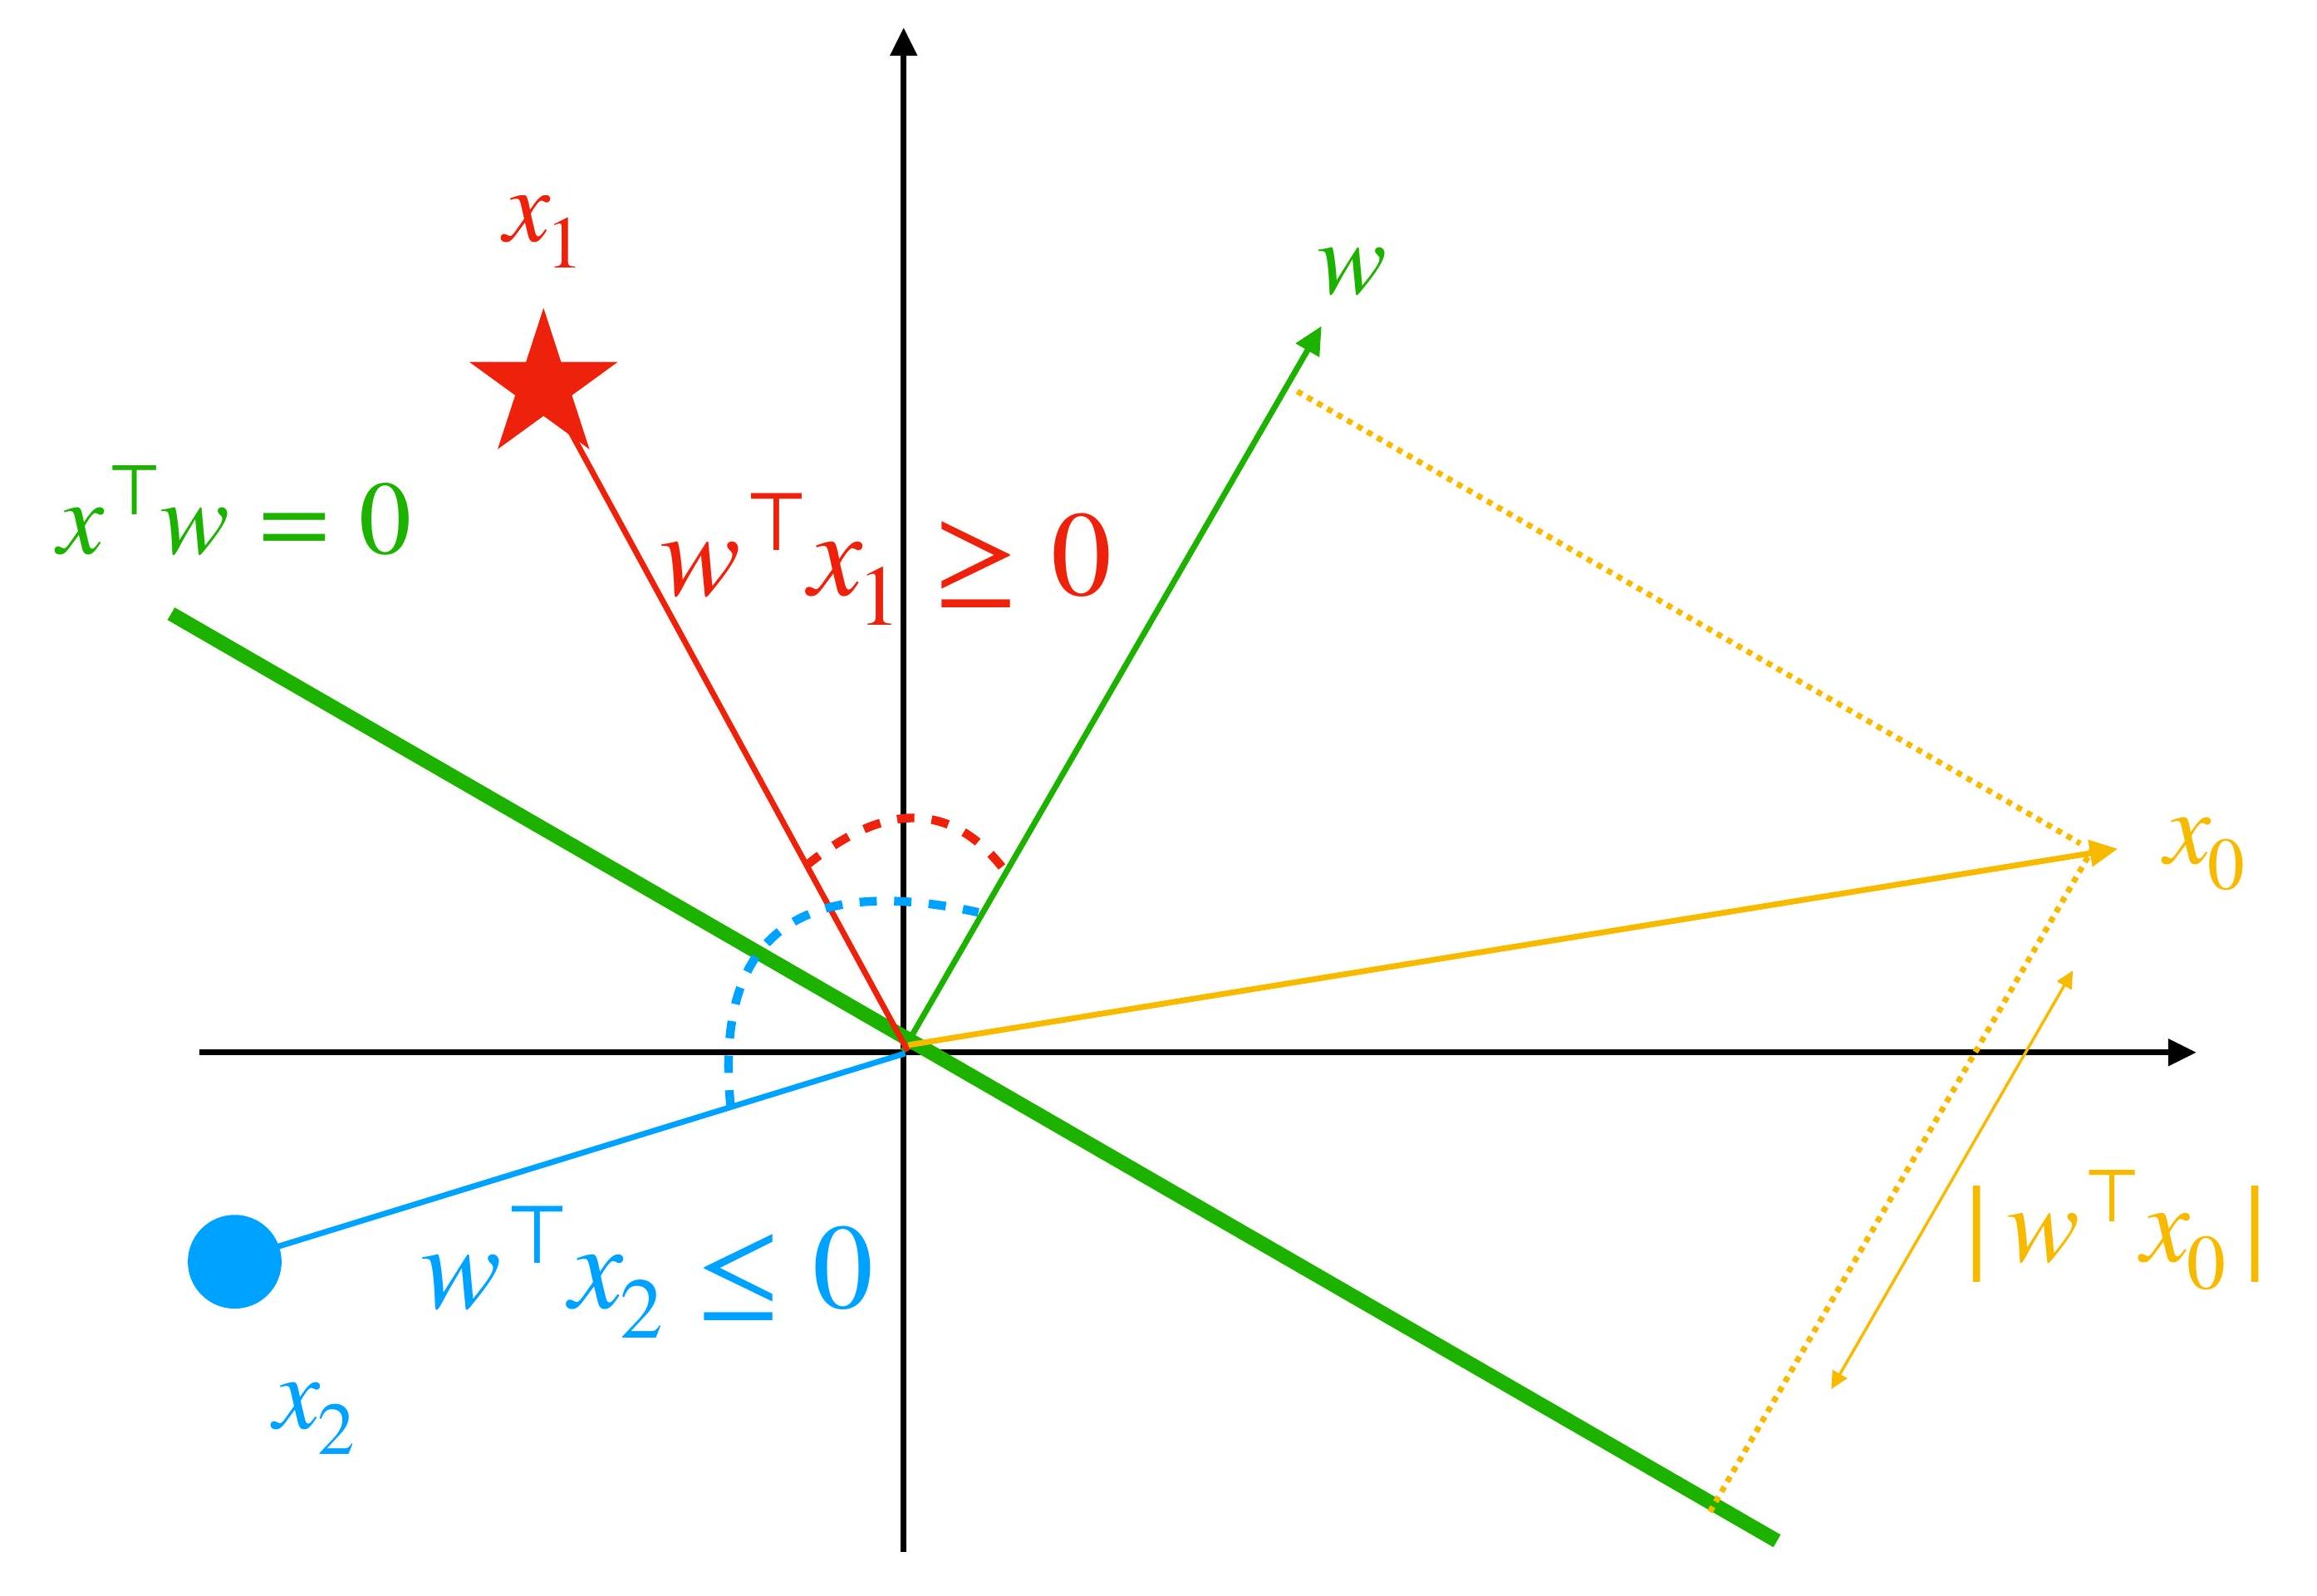
\includegraphics[width=0.6\columnwidth]{figures/hyperplane1.jpg}
\end{wrapfigure}

- Define a hyperplane as $\left\{x: w^{\top} x=0\right\}$ where $\|w\|=1$

- Prediction:

$
f(x)=\operatorname{sign}\left(x^{\top} w\right)
$

- Claim: The distance between a point $x_{0}$ and the hyperplane defined by $w$ is $\left|w^{\top} x_{0}\right|$

- Proof: The distance between $x_{0}$ and the hyperplane is given by $\min _{u: w^{\top} u=0}\left\|x_{0}-u\right\|$

Let $v=x_{0}-w^{\top} x_{0} w$ then by the Pythagorean theorem for any $u$ s.t. $w^{\top} u=0$

% \begin{wrapfigure}{r}{0.6\columnwidth} 
  % \centering
  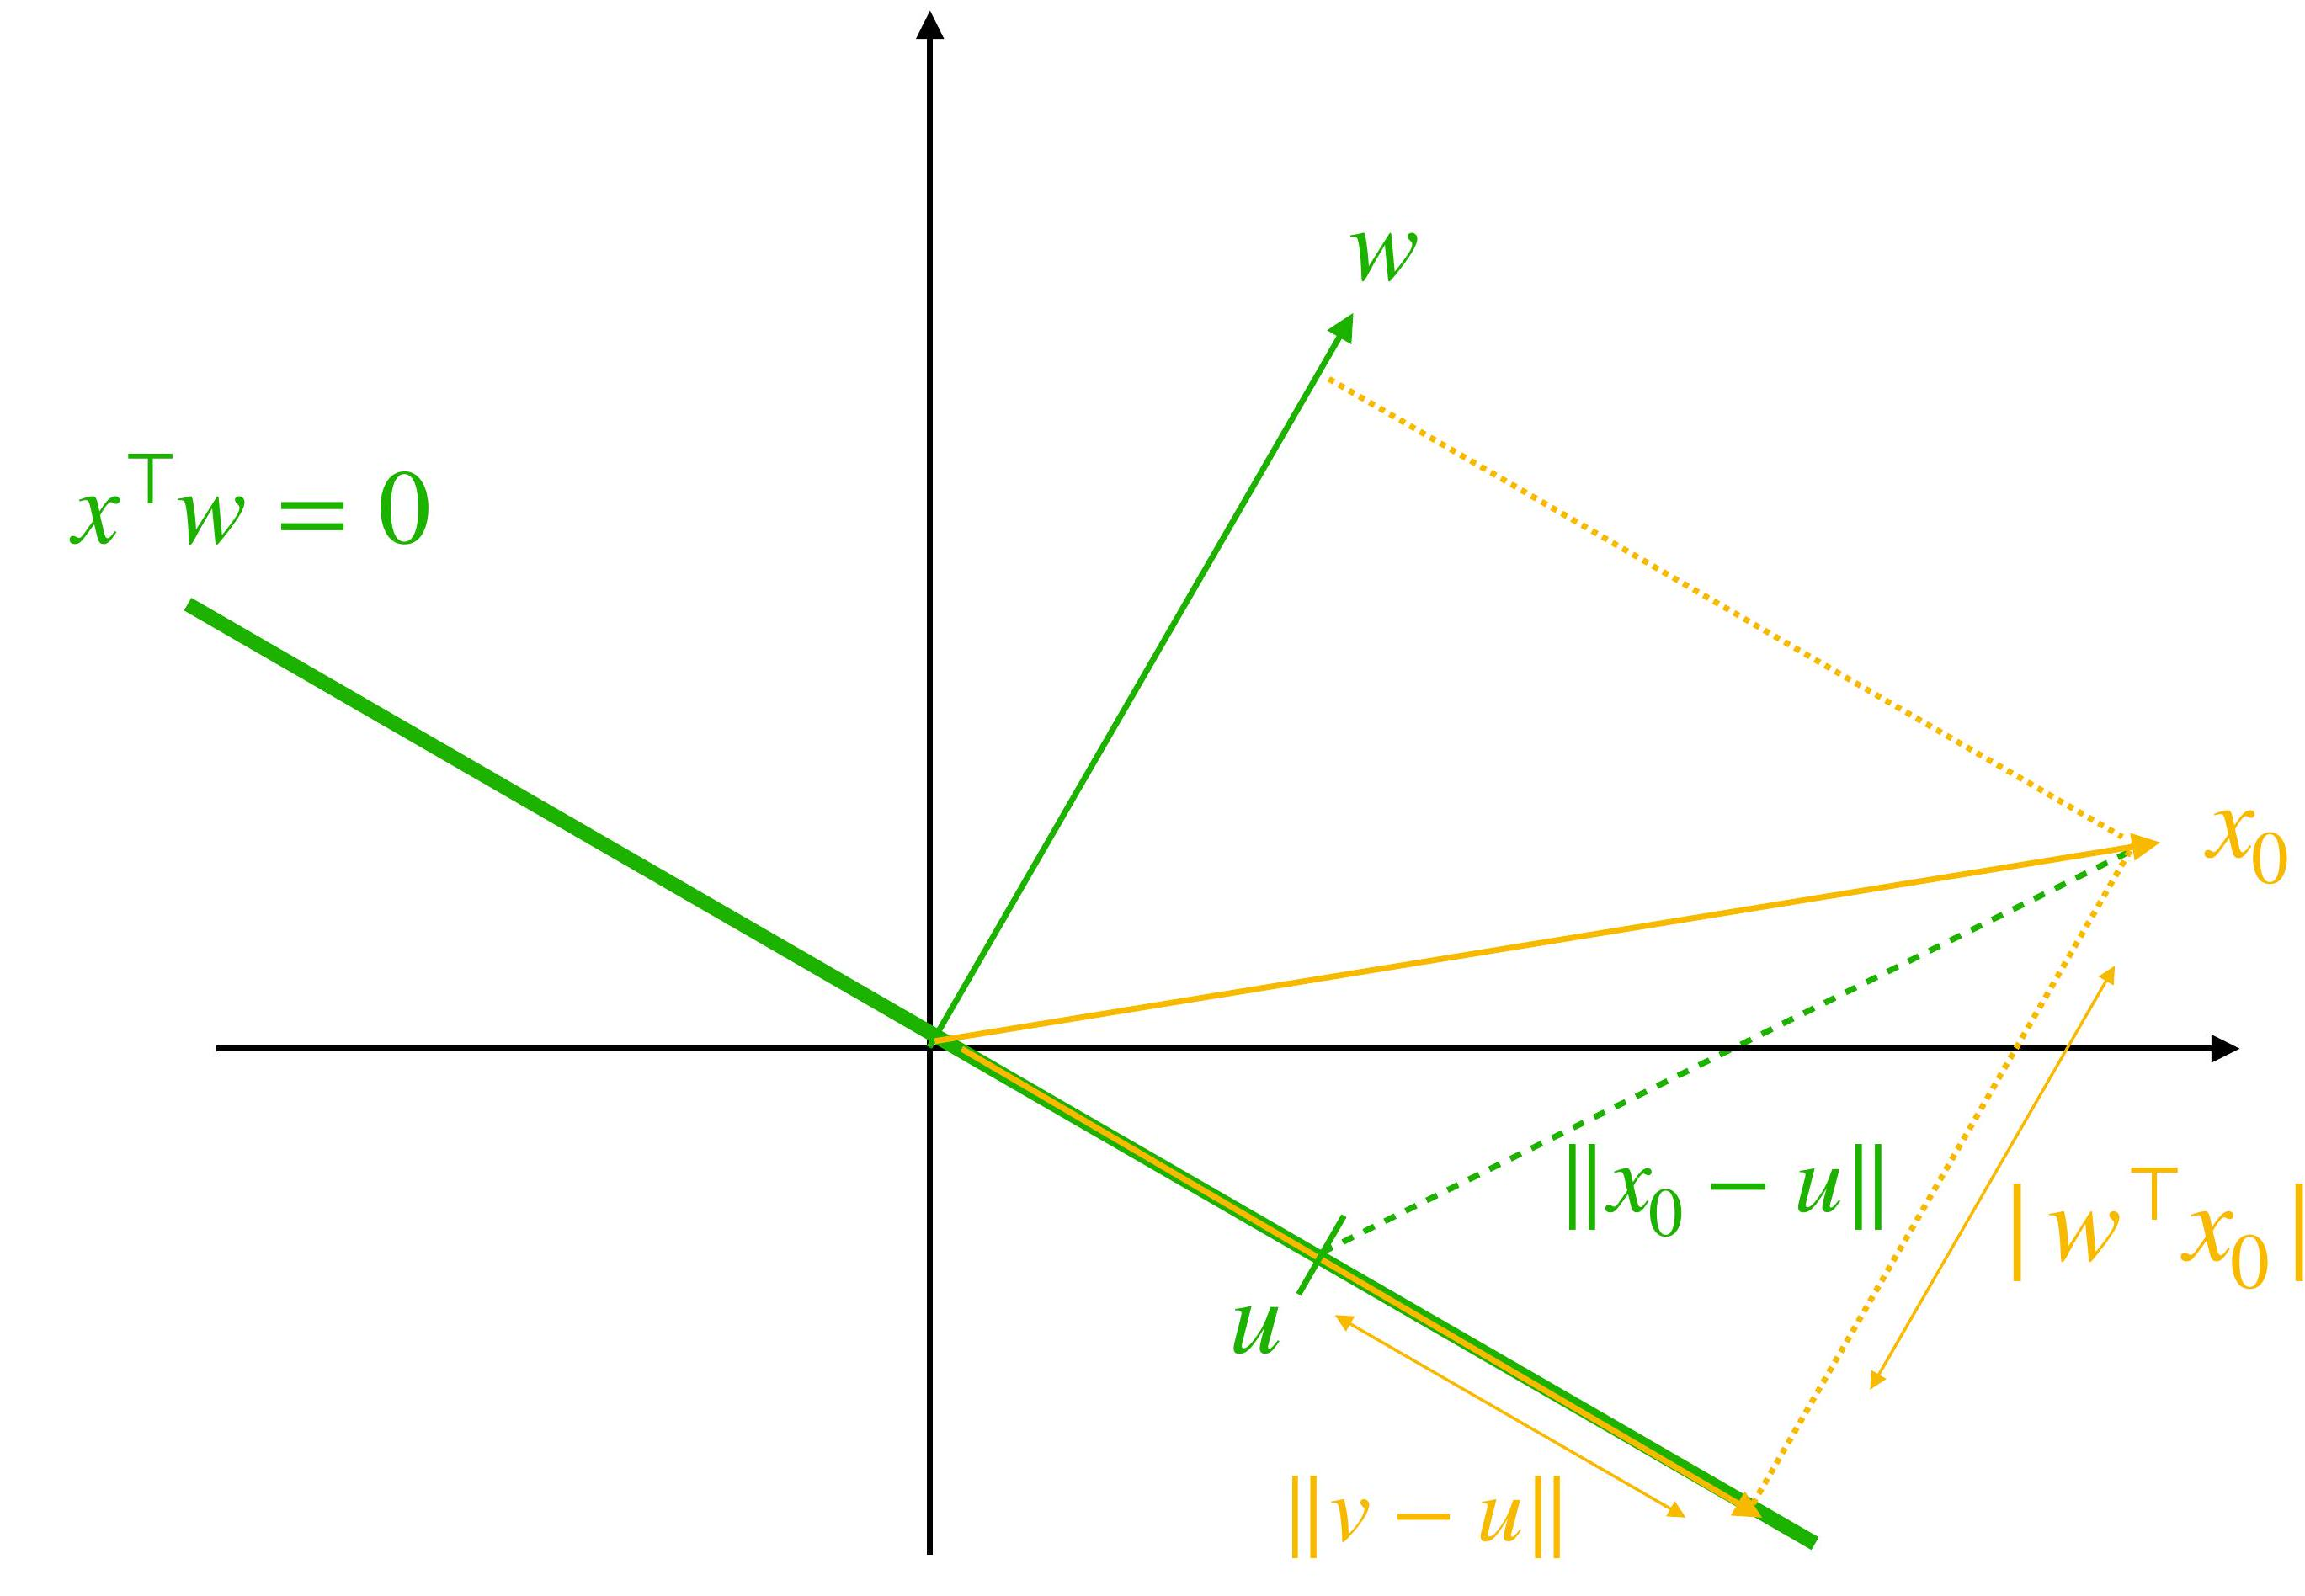
\includegraphics[width=0.9\columnwidth]{figures/hyperplane2.jpg}
% \end{wrapfigure}

$\left\|x_{0}-u\right\|^{2}=\left(w^{\top} x_{0}\right)^{2}+\|v-u\|^{2} \geq\left(w^{\top} x_{0}\right)^{2}$


\subsection*{Hard-SVM rule: max-margin separating hyperplane}

% \begin{wrapfigure}{r}{0.6\columnwidth} 
  % \centering
  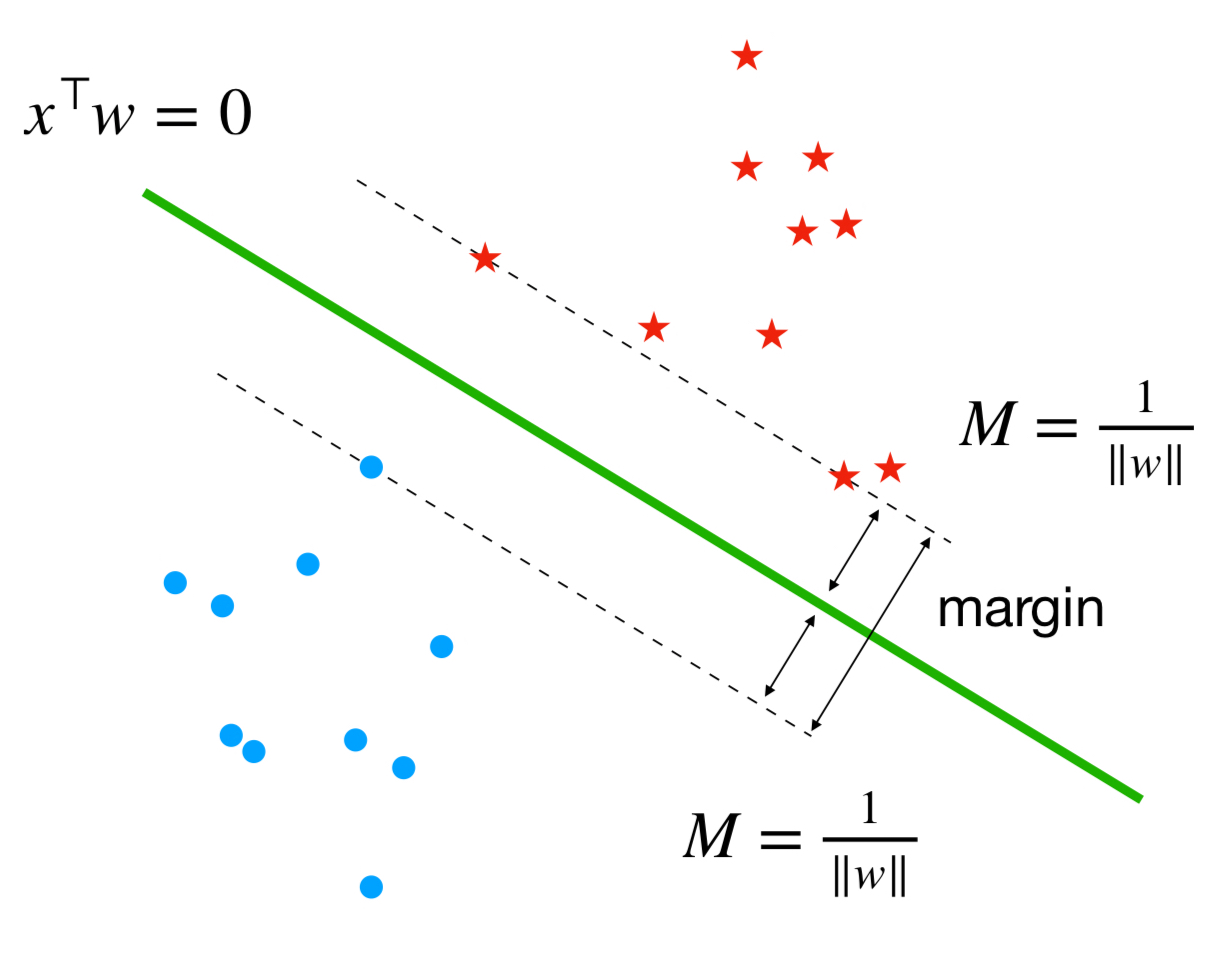
\includegraphics[width=0.8\columnwidth]{figures/hard_svm.jpeg}
% \end{wrapfigure}

- First assume the dataset $\left(x_{n}, y_{n}\right)_{n=1}^{N}$ is linearly separable

- Margin of a hyperplane: $\min _{n \leq N}\left|w^{\top} x_{n}\right|$

- Max-margin separating hyperplane:

$
\max _{w,\|w\|=1} \min _{n \leq N}\left|w^{\top} x_{n}\right| \text { s.t. } \forall n, y_{n} x_{n}^{\top} w \geq 0
$

- Equivalent to: \\$\max _{M \in \mathbb{R}, w,\|w\|=1} M$ s.t. $\forall n, y_{n} x_{n}^{\top} w \geq M$

- Also equivalent to:

$
\min _{w} \frac{1}{2}\|w\|^{2} \text { such that } \forall n, y_{n} x_{n}^{\top} w \geq 1
$

% \subsection*{Proof of the equivalent formulations}
% Claim: The following optimization problems are equivalent
% $\max \min \left|w^{\top} x_{n}\right|$
% $w,\|w\|=1 \quad n \leq N$
% s.t. $\forall n, y_{n} x_{n}^{\top} w \geq 0$
% $\max _{M \in \mathbb{R}, w,\|w\|=1} M$
% s.t. $\forall n, y_{n} x_{n}^{\top} w \geq M$

% Proof: Let $w_{1}$ be a solution of (I) and $M_{1}=\min _{n \leq N}\left|w_{1}^{\top} x_{n}\right|$ and let $w_{2}$ and $M_{2}$ be solutions of (II)

% \begin{itemize}
%   \item $\left(w_{1}, M_{1}\right)$ is admissible for (II) so $M_{1} \leq M_{2}$
%   \item $w_{2}$ is admissible for (I) so $\min _{n \leq N}\left|w_{2}^{\top} x_{n}\right| \leq \min _{n \leq N}\left|w_{1}^{\top} x_{n}\right|$
%   \item $\forall n, y_{n} x_{n}^{\top} w_{2} \geq M_{2}$ implies that $\forall n,\left|x_{n}^{\top} w_{2}\right| \geq M_{2}$ and $\min _{n \leq N}\left|x_{n}^{\top} w_{2}\right| \geq M_{2}$
% \end{itemize}

% Therefore $M_{1}=\min _{n \leq N}\left|w_{1}^{\top} x_{n}\right| \geq \min _{n \leq N}\left|w_{2}^{\top} x_{n}\right| \geq M_{2} \geq M_{1}$

% And the two problems are equivalent

% \subsection*{Proof of the equivalent formulations}
% Claim: The following optimization problems are equivalent

% $$
% \begin{aligned}
% & \max _{M \in \mathbb{R}, w,\|w\|=1} M \\
% & \text { s.t. } \forall n, y_{n} x_{n}^{\top} w \geq M \\
% & \min _{w} \frac{1}{2}\|w\|^{2} \\
% & \text { s.t. } \forall n, y_{n} x_{n}^{\top} w \geq 1
% \end{aligned}
% $$

% Proof:

% $$
% \begin{aligned}
% & \max _{M \in \mathbb{R}, w,\|w\|=1} M \text { such that } \forall n, y_{n} x_{n}^{\top} w \geq M \\
% \Longleftrightarrow & \max _{M \in \mathbb{R}, w} M \text { such that } \forall n, y_{n} x_{n}^{\top} \frac{w}{\|w\|} \geq M
% \end{aligned}
% $$

% The constraints are independent of the scale of $w$. Set $\|w\|=1 / M$ :

% $\Longleftrightarrow \max 1 /\|w\|$ such that $\forall n, y_{n} x_{n}^{\top} w \geq 1$

% $\Longleftrightarrow \min _{w}^{w} \frac{1}{2}\|w\|^{2}$ such that $\forall n, y_{n} x_{n}^{\top} w \geq 1$

\subsection*{Soft SVM}

% \begin{wrapfigure}{r}{0.6\columnwidth} 
  % \centering
  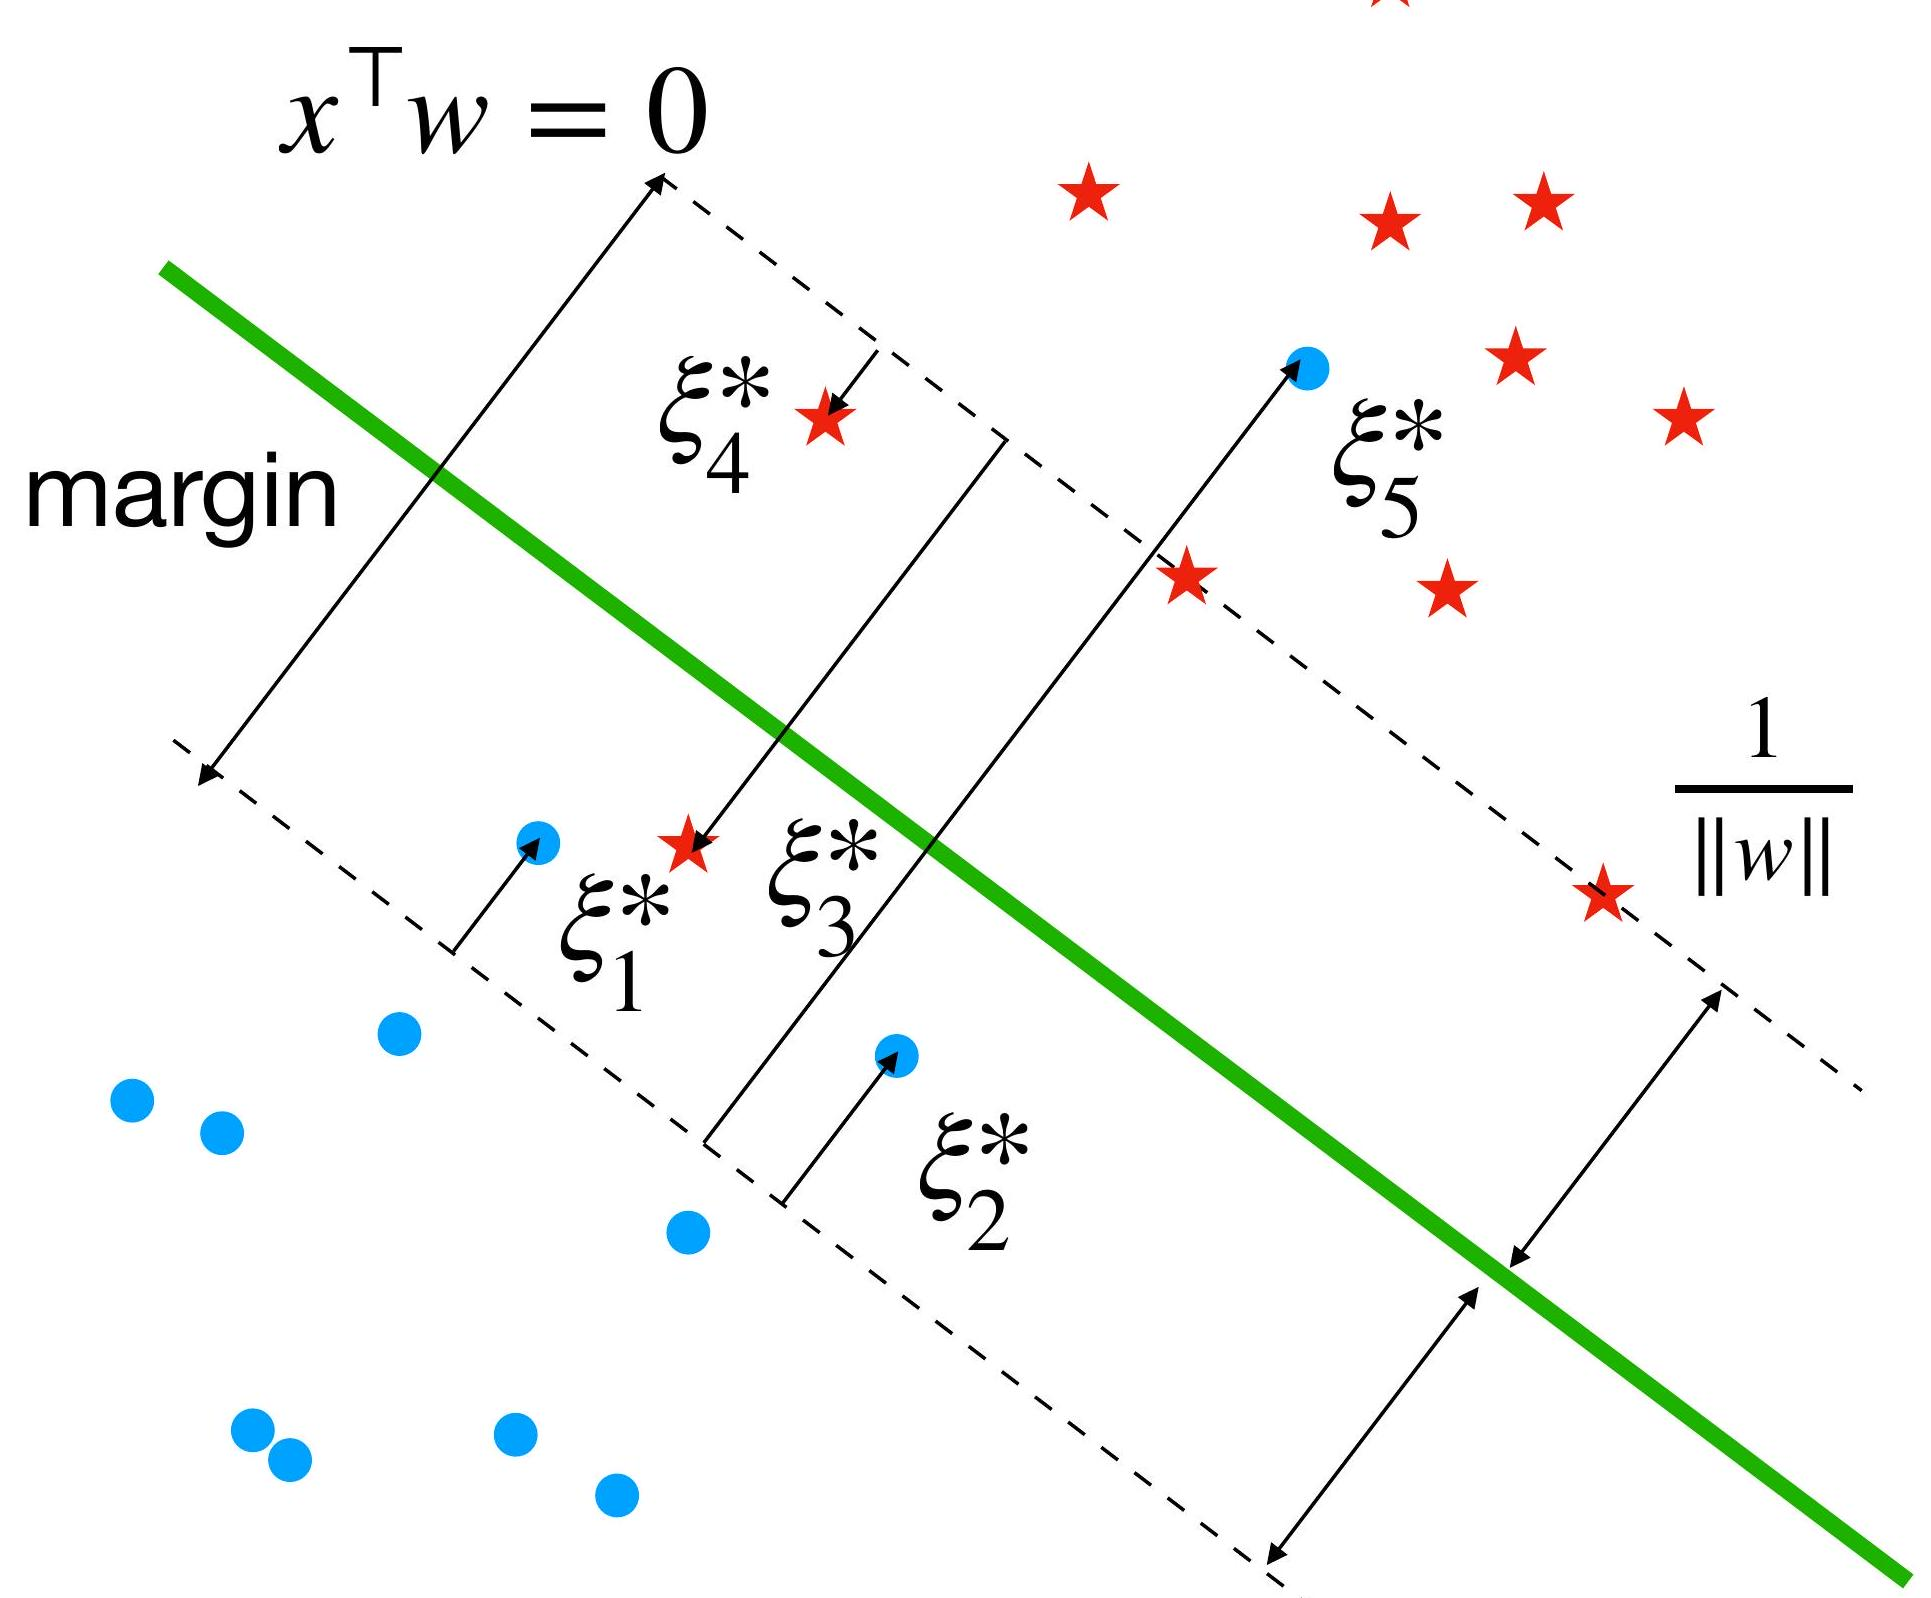
\includegraphics[width=0.7\columnwidth]{figures/soft_svm.jpg}
% \end{wrapfigure}

- A relaxation of the Hard-SVM rule that can be applied even if the training set is not linearly separable

- Idea: Maximize the margin while allowing some constraints to be violated

- Introduce positive slack variables $\xi_{1}, \cdots, \xi_{N}$ and replace the constraints with $y_{n} x_{n}^{\top} w \geq 1-\xi_{n}$ 

- Soft SVM:

$
\begin{aligned}
& \min _{w, \xi} \frac{\lambda}{2}\|w\|^{2}+\frac{1}{N} \sum_{n=1}^{N} \xi_{n} \\
& \text { s.t. } \forall n, y_{n} x_{n}^{\top} w \geq 1-\xi_{n} \text { and } \xi_{n} \geq 0
\end{aligned}
$

- Equivalent to:

$
\min _{w} \frac{\lambda}{2}\|w\|^{2}+\frac{1}{N} \sum_{n=1}^{N}\left[1-y_{n} x_{n}^{\top} w\right]_{+}
$

(A hinge loss)


$
\xi_{i}^{*}=\frac{\xi_{i}}{\|w\|}
$


 
- Proof: Fix $w$ and consider the minimization over $\xi$ :

1) If $y_{n} x_{n}^{\top} w \geq 1$, then $\xi_{n}=0$

2) If $y_{n} x_{n}^{\top} w<1, \xi_{n}=1-y_{n} x_{n}^{\top} w$

Therefore $\xi_{n}=\left[1-y_{n} x_{n}^{\top} w\right]_{+}$


\subsection*{Classification by risk minimization}
- $(X, Y) \sim \mathscr{D}$ with ranges $\mathscr{X}$ and $\mathscr{Y}=\{-1,1\}$

- Goal: Find a classifier $f: \mathscr{X} \rightarrow \mathcal{Y}$ that minimizes the true risk
$
L(f)=\mathbb{E}_{\mathscr{D}}\left(1_{Y \neq f(X)}\right)
$

- How: Through Empirical Risk Minimization (ERM):

$
\min _{w} L_{\text {train }}(w)=\frac{1}{N} \sum_{n=1}^{N} \phi\left(y_{n} w^{\top} x_{n}\right)
$

$\phi$ represents the loss function of the functional margin $y_{n} x_{n}^{\top} w$

$\phi$ also serves as a convex surrogate for the $0-1$ loss

\subsection*{Losses for Classification}
Examples of margin-based losses $\left(\eta=y x^{\top} w\right)$ :

\begin{itemize}
  \item Quadratic loss: $\operatorname{MSE}(\eta)=(1-\eta)^{2}$
  \item Logistic loss: $\operatorname{Logistic}(\eta)=\frac{\log (1+\exp (-\eta))}{\log (2)}$
  \item Hinge loss: $\operatorname{Hinge}(\eta)=[1-\eta]_{+}$
\end{itemize}

Common features: these losses are convex and provide an upper bound for the zero-one loss

Behavioral differences:

\begin{itemize}
  \item MSE: Penalizes any deviation from 1
  \item Logistic Loss: Asymmetric cost - a penalty is always incurred.
\end{itemize}


\begin{itemize}
  \item Hinge Loss: A penalty is applied if the prediction is incorrect or lacks confidence
\end{itemize}

\subsection*{Summary}
$$
\min _{w} \frac{\lambda}{2}\|w\|^{2}+\frac{1}{N} \sum_{n=1}^{N}\left[1-y_{n} x_{n}^{\top} w\right]_{+}
$$

ERM for the hinge loss with ridge regularization


Interpretation for separable data with small $\lambda$ :

\begin{enumerate}
  \item Choose the direction of $w$ such that $w^{\perp}$ acts as a separating hyperplane

  \item Adjust the scale of $w$ to ensure that no point lies with the margin

  \item Select the hyperplane with the largest margin

\end{enumerate}


\subsection*{Optimization: How to get $w$ ?}
$$
\min _{w} \frac{1}{N} \sum_{n=1}^{N}\left[1-y_{n} x_{n}^{\top} w\right]_{+}+\frac{\lambda}{2}\|w\|^{2}
$$

Convex (but non-smooth) objective which can be minimized with:

\begin{itemize}
  \item Subgradient method
  \item Stochastic Subgradient method
\end{itemize}

\subsection*{Convex duality}
Assume you can define an auxiliary function $G(w, \alpha)$ such that

$$
\min _{w} L(w)=\min _{w} \max _{\alpha} G(w, \alpha)
$$

Primal problem: $\min \max G(w, \alpha)$

w $\quad \alpha$

Dual problem: $\max \min G(w, \alpha)$

$\alpha \quad w$

$\Rightarrow$ Sometimes, the dual problem is easier to solve than the primal problem.

Questions:

\begin{enumerate}
  \item How do we identify a suitable $G(w, \alpha)$ ?

  \item Under what conditions can the min and max be interchanged?

  \item When is the dual problem more tractable than the primal problem?

\end{enumerate}

\subsection*{Q1: How do we find a suitable $G(w, \alpha)$ ?}
$$
[z]_{+}=\max (0, z)=\max _{\alpha \in[0,1]} \alpha z
$$

Therefore $\left[1-y_{n} x_{n}^{\top} w\right]_{+}=\max _{\alpha_{n} \in[0,1]} \alpha_{n}\left(1-y_{n} x_{n}^{\top} w\right)$

The SVM problem is equivalent to:

$$
\min _{w} L(w)=\min _{w} \max _{\alpha \in[0,1]^{n}} \underbrace{\frac{1}{N} \sum_{n=1}^{N} \alpha_{n}\left(1-y_{n} x_{n}^{\top} w\right)+\frac{\lambda}{2}\|w\|_{2}^{2}}_{G(w, \alpha)}
$$

The function $\mathrm{G}$ is convex in $w$ and concave in $\alpha$

\subsection*{Q2: Can the min and max be interchanged?}
Always true:

$$
\max _{\alpha} \min _{w} G(w, \alpha) \leq \min _{w} \max _{\alpha} G(w, \alpha)
$$

Equality if $G$ is convex in $w$, concave in $\alpha$ and the domains of $w$ and $\alpha$ are convex and compact:

$\max \min G(w, \alpha)=\min \max G(w, \alpha)$


\subsection*{Q2: Can the min and max be interchanged?}
Always true:

$\max \min G(w, \alpha) \leq \min \max G(w, \alpha)$

$\alpha \quad w$

w $\quad \alpha$

Proof:

$\min G(\alpha, w) \leq G\left(\alpha, w^{\prime}\right)$ for any $w^{\prime}$

$w$

$\max \min G(\alpha, w) \leq \max G\left(\alpha, w^{\prime}\right)$ for any $w^{\prime}$

$\alpha w$

$\max \min G(\alpha, w) \leq \min \max G\left(\alpha, w^{\prime}\right)$

$\alpha \quad w$

$w^{\prime} \quad \alpha$

\subsection*{Application to SVM}
For SVM, the condition is met, allowing us to interchange min and max:

$$
\min _{w} L(w)=\max _{\alpha \in[0,1]^{n}} \min _{w} \frac{1}{N} \sum_{n=1}^{N} \alpha_{n}\left(1-y_{n} x_{n}^{\top} w\right)+\frac{\lambda}{2}\|w\|_{2}^{2}
$$

Minimizer computation:

$$
\mathbf{Y}=\operatorname{diag}(\mathbf{y})
$$

$\nabla_{w} G(w, \alpha)=-\frac{1}{N} \sum_{n=1}^{N} \alpha_{n} y_{n} x_{n}+\lambda w=0 \Longrightarrow w(\alpha)=\frac{1}{\lambda N} \sum_{n=1}^{N} \alpha_{n} y_{n} x_{n}=\frac{1}{\lambda N} \mathbf{X}^{\top} \mathbf{Y} \alpha$

Dual optimization problem:

$$
\begin{aligned}
\min _{w} L(w) & =\max _{\alpha \in[0,1]^{n}} \frac{1}{N} \sum_{n=1}^{N} \alpha_{n}\left(1-\frac{1}{\lambda N} y_{n} x_{n}^{\top} \mathbf{X}^{\top} \mathbf{Y} \alpha\right)+\frac{1}{2 \lambda N^{2}}\left\|\mathbf{X}^{\top} \mathbf{Y} \alpha\right\|_{2}^{2} \\
& =\max _{\alpha \in[0,1]^{n}} \frac{1^{\top} \alpha}{N}-\frac{1}{\lambda N^{2}} \alpha^{\top} \mathbf{Y} \mathbf{X} \mathbf{X}^{\top} \mathbf{Y} \alpha+\frac{1}{2 \lambda N^{2}}\left\|\mathbf{X}^{\top} \mathbf{Y} \alpha\right\|_{2}^{2} \\
& =\max _{\alpha \in[0,1]^{n}} \frac{1^{\top} \alpha}{N}-\frac{1}{2 \lambda N^{2}} \alpha^{\top} \underbrace{\mathbf{Y} \mathbf{X} \mathbf{X}^{\top} \mathbf{Y}}_{\text {PSD matrix }} \alpha
\end{aligned}
$$

\subsection*{Q3: Why?}
$$
\max _{\alpha \in[0,1]^{n}} \alpha^{\top} 1-\frac{1}{2 \lambda N} \alpha^{\top} \underbrace{\mathbf{Y X} \mathbf{X}^{\top} \mathbf{Y}}_{\text {PSD matrix }} \alpha
$$

\begin{enumerate}
  \item Differentiable Concave Problem: Efficient solutions can be achieved using
\end{enumerate}

\begin{itemize}
  \item Quadratic programming solvers
  \item Coordinate ascent
\end{itemize}

\begin{enumerate}
  \setcounter{enumi}{1}
  \item Kernel Matrix Dependency: The cost function only depends on the data via the kernel matrix $K=\mathbf{X} \mathbf{X}^{\top} \in \mathbb{R}^{N \times N}$ - no dependency on $d$

  \item Dual Formulation Insight: $\alpha$ is typically sparse and non-zero exclusively for the training examples that are crucial in determining the decision boundary

\end{enumerate}

\subsection*{Interpretation of the dual formulation}
For any $\left(x_{n}, y_{n}\right)$, there is a corresponding $\alpha_{n}$ given by

$$
\max _{\alpha_{n} \in[0,1]} \alpha_{n}\left(1-y_{n} x_{n}^{\top} w\right)
$$

\begin{itemize}
  \item If $x_{n}$ is on the correct side and outside the margin, $1-y_{n} x_{n}^{\top} w<0$, then $\alpha_{n}=0$
  \item If $x_{n}$ is on the correct side and on the margin, $1-y_{n} x_{n}^{\top} w=0$, then $\alpha_{n} \in[0,1]$
  \item If $x_{n}$ is strictly inside the margin or or the incorrect side, $1-y_{n} x_{n}^{\top} w>0$, then $\alpha_{n}=1$
\end{itemize}

$\rightarrow$ The points for which $\alpha_{n}>0$ are referred to as support vectors

$$
\left(\alpha_{n}=0 \text { and } y_{n}=-1\right) \text { or }\left(\alpha_{n}=1 \text { and } y_{n}=1\right) \quad{ }_{w^{\top} x=-1} w^{\top} x=0
$$

\subsection*{The SVM hyperplane is supported by}
 the support vectors$$
\left(\alpha_{n}=0 \text { and } y_{n}=1\right) \text { or }\left(\alpha_{n}=1 \text { and } y_{n}=-1\right)
$$

$$
w=\frac{1}{\lambda N} \sum_{n=1}^{N} \alpha_{n} y_{n} x_{n}
$$

$\Rightarrow w$ does not depend on the observation $\left(x_{n}, y_{n}\right)$ if $\alpha_{n}=0$

$$
\left(\alpha_{n}=0 \text { and } y_{n}=-1\right) \text { or }\left(\alpha_{n}=1 \text { and } y_{n}=1\right)
$$

$$
w^{\top} x=-1 \quad w^{\top} x=0
$$

\subsection*{Recap}
\begin{itemize}
  \item Hard SVM - finds max-margin separating hyperplane $\min _{w} \frac{1}{2}\|w\|^{2}$ such that $\forall n, y_{n} x_{n}^{\top} w \geq 1$

  \item Soft SVM - relax the constraint for non-separable data

\end{itemize}

$$
\min _{w} \frac{\lambda}{2}\|w\|^{2}+\frac{1}{N} \sum_{n=1}^{N}\left[1-y_{n} x_{n}^{\top} w\right]_{+}
$$

\begin{itemize}
  \item Hinge loss can be optimized with (stochastic) sub-gradient method

  \item Duality: min max problem is equivalent to max min (convex-concave objective)

  \item Efficient solutions with quadratic programming and coordinate ascent

  \item The cost depends on the data via the kernel matrix (no dependency on $d$ )

\end{itemize}
\sectiondivider

\sectionnewcolor

\section*{Supervised machine learning}
We observe some data $S_{\text {train }}=\left\{x_{n}, y_{n}\right\}_{n=1}^{N} \in \mathscr{X} \times \mathscr{Y}$

Goal: given a new observation $x$, we want to predict its label $y$

How:


\section*{Nearest neighbor function}
$$
\begin{aligned}
\operatorname{nbh}_{S_{\text {train }}, k}: X & \rightarrow X^{k} \\
x & \mapsto\left\{\text { the } k \text { elements of } S_{\text {train }} \text { closest to } x\right\}
\end{aligned}
$$


\section*{Nearest neighbor function}
$$
\begin{aligned}
\mathrm{nbh}_{S_{\text {train }}, k}: X & \rightarrow \mathscr{X}^{k} \\
x & \mapsto\left\{\text { the } k \text { elements of } S_{\text {train }} \text { closest to } x\right\}
\end{aligned}
$$


$\operatorname{nbh}_{S_{\text {train }}, 3}(x)=$ ?

\section*{Nearest neighbor function}
$$
\begin{aligned}
\mathrm{nbh}_{S_{\text {train }}, k}: X & \rightarrow \mathscr{X}^{k} \\
x & \mapsto\left\{\text { the } k \text { elements of } S_{\text {train }} \text { closest to } x\right\}
\end{aligned}
$$


$\operatorname{nbh}_{S_{\text {train }}, 3}(x)=\left\{x_{3}, x_{4}, x_{7}\right\}$

\section*{Nearest neighbor function}
$$
\begin{aligned}
\mathrm{nbh}_{S_{\text {train }}, k}: X & \rightarrow \mathscr{X}^{k} \\
x & \mapsto\left\{\text { the } k \text { elements of } S_{\text {train }} \text { closest to } x\right\}
\end{aligned}
$$


$\operatorname{nbh}_{S_{\text {train }}, 2}(x)=?$

\section*{Nearest neighbor function}
$$
\begin{aligned}
\mathrm{nbh}_{S_{\text {train }}, k}: X & \rightarrow \mathscr{X}^{k} \\
x & \mapsto\left\{\text { the } k \text { elements of } S_{\text {train }} \text { closest to } x\right\}
\end{aligned}
$$


$\operatorname{nbh}_{S_{\text {train }}, 2}(x)=?$

\section*{Nearest neighbor function}
$$
\mathrm{nbh}_{S_{\text {train }, k}}: \mathscr{X} \rightarrow \mathscr{X}^{k}
$$

$x \mapsto\left\{\right.$ the $k$ elements of $S_{\text {train }}$ closest to $\left.x\right\}$


$$
\mathrm{nbh}_{S_{\text {train }}, 2}(x)=\left\{x_{5}, x_{8}\right\}
$$

\section*{Nearest neighbor function}
$$
\begin{aligned}
\mathrm{nbh}_{S_{\text {train }}, k}: X & \rightarrow \mathscr{X}^{k} \\
x & \mapsto\left\{\text { the } k \text { elements of } S_{\text {train }} \text { closest to } x\right\}
\end{aligned}
$$


Remarks:

\begin{itemize}
  \item Different metrics can be employed
  \item High computational complexity for large $N$ (but efficient data structure may exist)
\end{itemize}

\section*{k-NN can be used for regression $(y \in \mathbb{R})$}
$$
f_{S_{\text {train }}, k}(x)=\frac{1}{k} \sum_{n: x_{n} \in n b h_{S_{\text {train }, k}}(x)} y_{n}
$$


\section*{k-NN can be used for regression $(y \in \mathbb{R})$}
$$
f_{S_{\text {train }}, k}(x)=\frac{1}{k} \sum_{n: x_{n} \in n b h_{S_{\text {train }, k}(x)}} y_{n}
$$


$$
f_{S_{\text {train }}, 3}(x)=?
$$

\section*{k-NN can be used for regression $(y \in \mathbb{R})$}
$$
f_{S_{\text {train }}, k}(x)=\frac{1}{k} \sum_{n: x_{n} \in n b h_{S_{\text {train }, k}(x)}} y_{n}
$$


\section*{k-NN can be used for regression $(y \in \mathbb{R})$}
$$
f_{S_{\text {train }}, k}(x)=\frac{1}{k} \sum_{n: x_{n} \in n b h_{S_{\text {train }, k}(x)}} y_{n}
$$


\section*{k-NN can be used for classification $(y \in\{0,1\}$ )}
$$
f_{S_{\text {train }, k}}(x)=\operatorname{majority}\left\{y_{n}: x_{n} \in \operatorname{nbh}_{S_{\text {train }, ~}}(x)\right\}
$$


\section*{k-NN can be used for classification $(y \in\{0,1\}$ )}
$$
f_{S_{\text {train }, k}}(x)=\operatorname{majority}\left\{y_{n}: x_{n} \in \operatorname{nbh}_{S_{\text {train }, ~}}(x)\right\}
$$


$$
f_{S_{\text {train }, 1}}(x)=?
$$

\section*{k-NN can be used for classification $(y \in\{0,1\}$ )}
$$
f_{S_{\text {train }, k}}(x)=\operatorname{majority}\left\{y_{n}: x_{n} \in \operatorname{nbh}_{S_{\text {train }, ~}}(x)\right\}
$$


$$
f_{S_{\text {train } 1}}(x)=1
$$

\section*{k-NN can be used for classification $(y \in\{0,1\}$ )}
$$
f_{S_{\text {train }, k}}(x)=\operatorname{majority}\left\{y_{n}: x_{n} \in \operatorname{nbh}_{S_{\text {train }, ~}}(x)\right\}
$$


$$
f_{S_{\text {train } 3}}(x)=?
$$

\section*{k-NN can be used for classification $(y \in\{0,1\}$ )}
$$
f_{S_{\text {train }, k}}(x)=\operatorname{majority}\left\{y_{n}: x_{n} \in \operatorname{nbh}_{S_{\text {train }, ~}}(x)\right\}
$$


$$
f_{S_{\text {train } 3}}(x)=0
$$

\section*{k-NN can be used for classification $(y \in\{0,1\}$ )}
$$
f_{S_{\text {train }, k}}(x)=\operatorname{majority}\left\{y_{n}: x_{n} \in \operatorname{nbh}_{S_{\text {train }, ~}}(x)\right\}
$$


$$
f_{S_{\text {train } 4}}(x)=? \text { Tie! }
$$

\section*{k-NN can be used for classification $(y \in\{0,1\})$}
$$
f_{S_{\text {train }, k}}(x)=\text { majority }\left\{y_{n}: x_{n} \in \operatorname{nbh}_{S_{\text {train }}, k}(x)\right\}
$$


Remarks:

\begin{itemize}
  \item Choose an odd value for $\mathrm{k}$ to prevent ties
  \item Generalization: smoothing kernels; weighted linear combination of elements
\end{itemize}

\section*{Why does it make sense?}
\begin{itemize}
  \item Relevant in the presence of spatial correlation

  \item Implicitly models intricate decision boundaries in low-dimensional spaces

\end{itemize}


\section*{Bias-variance tradeoff in k-NN}
For small k:

\begin{itemize}
  \item Low bias - complex decision boundary
  \item High variance - overfitting
\end{itemize}

For large k:

(When $k=N$, prediction is constant)

\begin{itemize}
  \item High bias
  \item Low variance
\end{itemize}


1-nearest neighbor classification

\section*{U-shaped curve for $\mathrm{k}-\mathrm{NN}$ bias-variance tradeoff}

Complexity increases as $k$ decreases

\section*{Find a $k$ that balances bias and variance}
Characteristics of an optimal k:

\begin{itemize}
  \item Low bias: Ensures a sufficiently complex decision boundary
  \item Low variance: Prevents overfitting
\end{itemize}


\section*{Summary: k-Nearest Neighbor}
\section*{Pros:}
\begin{itemize}
  \item No optimization or training
  \item Easy to implement
  \item Works well in low dimensions, allowing for very complex decision boundaries
\end{itemize}

Cons:

\begin{itemize}
  \item Slow at query time
  \item Not suitable for high-dimensional data
  \item Choosing the right local distance is crucial
\end{itemize}


\section*{Curse of dimensionality}
Claim 1: As the dimensionality grows, fixed-size training sets cover a diminishing fraction of the input space

Assume the data $x \sim \mathcal{U}\left([0,1]^{d}\right)$

Consider a blue box around the center $x_{0}$ of size $r$

$$
\mathbb{P}(x \in)=r^{d}:=\alpha
$$

If $\alpha=0.01$, to have:

$$
\begin{aligned}
& d=10, \text { we need } r=0.63 \\
& d=100, \text { we need } r=0.95
\end{aligned}
$$

We need to explore almost the whole box


$X=[0,1]^{d}$

\section*{Curse of dimensionality}
Claim 2: In high-dimension, data-points are far from each other.

Consider $N$ i.i.d. points uniform in the $[0,1]^{d}$

$$
\mathbb{P}\left(\exists x_{i} \in \square\right) \geq 1 / 2 \Longrightarrow r \geq\left(1-\frac{1}{2^{1 / N}}\right)^{1 / d}
$$

Proof: $\mathbb{P}(x \notin \square)=1-r^{d}$

$$
\begin{aligned}
& \mathbb{P}\left(x_{i} \notin \quad, \forall i \leq N\right)=\left(1-r^{d}\right)^{N} \\
& \mathbb{P}\left(\exists x_{i} \in \square\right)=1-\left(1-r^{d}\right)^{N}
\end{aligned}
$$

For $d=10, N=500$, we have $r \geq 0.52$


$$
\mathscr{X}=[0,1]^{d}
$$

\section*{Generalization bound for 1-NN}
Setup: $(X, Y) \sim \mathscr{D}$ over $\mathscr{X} \times \mathscr{Y}=[0,1]^{d} \times\{0,1\}$

Goal: Bound the classification error:

$$
L(f)=\mathbb{P}_{(X, Y) \sim D}(Y \neq f(X))
$$

Baseline:

\begin{itemize}
  \item Bayes classifier: minimizes $L$ over all classifiers
\end{itemize}

$$
f_{*}(x)=1_{\eta(x) \geq 1 / 2} \text { where } \eta(x)=\mathbb{P}(Y=1 \mid X=x)
$$

\begin{itemize}
  \item Bayes risk: represents the minimum probability of misclassification
\end{itemize}

$$
L\left(f_{*}\right)=\mathbb{P}\left(f_{*}(X) \neq Y\right)=\mathbb{E}_{X \sim D_{X}}[\min \{\eta(X), 1-\eta(X)\}]
$$

\section*{Generalization bound for 1-NN}

\begin{itemize}
  \item Bayes classifier: minimizes $L$ over all classifiers
\end{itemize}

$$
f_{*}(x)=1_{\eta(x) \geq 1 / 2} \text { where } \eta(x)=\mathbb{P}(Y=1 \mid X=x)
$$

\begin{itemize}
  \item Bayes risk: represents the minimum probability of misclassification
\end{itemize}

$$
L\left(f_{*}\right)=\mathbb{P}\left(f_{*}(X) \neq Y\right)=\mathbb{E}_{X \sim \mathscr{D}_{X}}[\min \{\eta(X), 1-\eta(X)\}]
$$

\section*{Generalization bound for 1-NN}
Proof 2:

$$
\begin{aligned}
& L\left(f_{*}\right)=\mathbb{E}_{(X, Y) \sim \mathscr{D}}\left[1_{f_{*}(X) \neq Y}\right]
\end{aligned}
$$


$$
\begin{aligned}
& =\mathbb{E}_{X \sim \mathscr{D}_{X}}\left[\mathbb{E}_{Y \sim \mathscr{D}_{Y \mid X}}\left[1_{f_{*}(X) \neq Y} \mid X\right] 1_{\eta(X) \geq 1 / 2}+E_{Y \sim \mathscr{D}_{Y \mid X}}\left[1_{f_{*}(X) \neq Y} \mid X\right] 1_{\eta(X)<1 / 2}\right] \\
& =\mathbb{E}_{X \sim \mathscr{D}_{X}}\left[\mathbb{E}_{Y \sim \mathscr{D}_{Y \mid X}}\left[1_{1 \neq Y} \mid X\right] 1_{\eta(X) \geq 1 / 2}+E_{Y \sim \mathscr{D}_{Y \mid X}}\left[1_{0 \neq Y} \mid X\right] 1_{\eta(X)<1 / 2}\right] \\
& =\mathbb{E}_{X \sim D_{X}}\left[\mathbb{P}(Y=0 \mid X) 1_{\eta(X) \geq 1 / 2}+\mathbb{P}(Y=1 \mid X) 1_{\eta(X)<1 / 2}\right] \\
& =\mathbb{E}_{X \sim \mathscr{D}_{X}}[\min \{\eta(X), 1-\eta(X)\}]
\end{aligned}
$$

\begin{itemize}
  \item Bayes risk: represents the minimum probability of misclassification
\end{itemize}

$$
L\left(f_{*}\right)=\mathbb{P}\left(f_{*}(X) \neq Y\right)=\mathbb{E}_{X \sim D_{X}}[\min \{\eta(X), 1-\eta(X)\}]
$$

\section*{Generalization bound for 1-NN}
Assumption: $\exists c \geq 0, \forall x, x^{\prime} \in \mathscr{X}$ :

$$
\left|\eta(x)-\eta\left(x^{\prime}\right)\right| \leq c\left\|x-x^{\prime}\right\|_{2}
$$

$\Rightarrow$ Nearby points are likely to share the same label

Claim:

$$
\leq 2 L\left(f_{*}\right)+4 c \sqrt{d} N^{-\frac{1}{d+1}}
$$


Interpretation:

For constant $d$ and $N \rightarrow \infty: \mathbb{E}_{S_{\text {train }}}\left[L\left(f_{S_{\text {train }}}\right)\right] \leq 2 L\left(f_{*}\right)$

geometric term: average distance between a random point and its closest neighbor

To achieve a constant error, we need $N \propto d^{(d+1) / 2}$ - curse of dimensionality

Despite common belief: Interpolation method can generalize well

\section*{Proof}
We want to bound

$$
\mathbb{E}_{S_{\text {train }}}\left[L\left(f_{S_{\text {train }}}\right)\right]=\mathbb{E}_{S_{\text {train }}}\left[\mathbb{P}_{(X, Y) \sim \mathscr{D}}\left[f_{S_{\text {train }}}(X) \neq Y\right]\right]
$$

We first sample $N$ unlabeled examples $S_{\text {train }, X}=\left(X_{1}, \cdots X_{N}\right) \sim \mathscr{D}_{X}$, an unlabeled example $X \sim \mathscr{D}_{X}$ and define $X^{\prime}=\operatorname{nbh}_{S_{\text {train }, 1}}(X)$

Finally we sample $Y \sim \eta(X)$ and $Y^{\prime} \sim \eta\left(X^{\prime}\right)$

We have:

$$
\begin{aligned}
& \mathbb{E}_{S_{\text {train }}}\left[L\left(f_{S_{\text {train }}}\right)\right]=\mathbb{E}_{S_{\text {train }, X}, X \sim D_{X}, Y \sim \eta(X), Y^{\prime} \sim \eta\left(X^{\prime}\right)}\left[1_{Y \neq f_{S_{\text {train }}(X)}}\right] \\
& =\mathbb{E}_{S_{\text {train, } X}, X \sim \mathscr{D}_{X}, Y \sim \eta(X), Y^{\prime} \sim \eta\left(X^{\prime}\right)}\left[1_{Y \neq Y^{\prime}}\right] \\
& =\mathbb{E}_{S_{\text {train }, X}, X \sim \mathscr{D}_{X}}\left[\mathbb{P}_{Y \sim \eta(X), Y^{\prime} \sim \eta\left(X^{\prime}\right)}\left(Y \neq Y^{\prime}\right)\right]
\end{aligned}
$$

\section*{Proof}
Consider two points $x, x^{\prime} \in[0,1]^{d}$.

Sample their labels $Y \sim \eta(x)$ and $Y^{\prime} \sim \eta\left(x^{\prime}\right)$

Claim:

$$
\mathbb{P}\left(Y^{\prime} \neq Y\right) \leq 2 \min \{\eta(x), 1-\eta(x)\}+c\left\|x-x^{\prime}\right\|
$$

\begin{itemize}
  \item Simple case: $x=x^{\prime}$
\end{itemize}

$$
\begin{aligned}
\mathbb{P}\left(Y^{\prime} \neq Y\right) & =\mathbb{E}\left[1_{Y^{\prime} \neq Y} 1_{Y^{\prime}=1}+1_{Y^{\prime} \neq Y^{\prime}} 1_{Y^{\prime}=0}\right] \\
& =\mathbb{P}\left(Y^{\prime}=1\right) \mathbb{P}(Y=0)+\mathbb{P}\left(Y^{\prime}=1\right) \mathbb{P}(Y=0) \\
& =2 \eta(x)(1-\eta(x)) \\
& \leq 2 \min \{\eta(x), 1-\eta(x)\}
\end{aligned}
$$

Case 1:

$\mathbf{Y}=\mathbf{0}(1-\eta(x))$

$Y^{\prime}=1 \quad \eta(x)$

Case 2:

$\mathrm{Y}=\mathbf{1} \quad \eta(x)$

$Y^{\prime}=0 \quad(1-\eta(x))$

\section*{Proof}
\begin{itemize}
  \item General case:
\end{itemize}

$$
\begin{aligned}
\mathbb{P}\left(Y \neq Y^{\prime}\right)= & \eta(x)\left(1-\eta\left(x^{\prime}\right)\right)+\eta\left(x^{\prime}\right)(1-\eta(x)) \\
= & \eta(x)(1-\eta(x))+\eta(x)\left(\eta(x)-\eta\left(x^{\prime}\right)\right) \\
& \quad+\eta(x)(1-\eta(x))+\left(\eta\left(x^{\prime}\right)-\eta(x)\right)(1-\eta(x)) \\
= & 2 \eta(x)(1-\eta(x))+(2 \eta(x)-1)\left(\eta(x)-\eta\left(x^{\prime}\right)\right) \\
& \leq 2 \eta(x)(1-\eta(x))+|(2 \eta(x)-1)|\left|\eta(x)-\eta\left(x^{\prime}\right)\right| \\
& \leq 2 \eta(x)(1-\eta(x))+\left|\eta(x)-\eta\left(x^{\prime}\right)\right| \\
& \leq 2 \eta(x)(1-\eta(x))+c\left\|x-x^{\prime}\right\| \\
& \leq 2 \min \{\eta(x), 1-\eta(x)\}+c\left\|x-x^{\prime}\right\|
\end{aligned}
$$

\section*{Proof}
$$
\begin{aligned}
\mathbb{E}_{S_{\text {train }}}\left[L \left(f_{\left.\left.S_{\text {train }}\right)\right]}\right.\right. & =\mathbb{E}_{S_{\text {train, }, X}, X \sim \mathscr{D}_{X}, Y \sim \eta(X), Y^{\prime} \sim \eta\left(X^{\prime}\right)}\left[1_{Y \neq f_{\text {train }(X)}}\right] \\
& =\mathbb{E}_{S_{\text {train, }, X}, X \sim \mathscr{D}_{X}, Y \sim \eta(X), Y^{\prime} \sim \eta\left(X^{\prime}\right)}\left[1_{Y \neq Y^{\prime}}\right] \\
& =\mathbb{E}_{S_{\text {train }, X}, X \sim D_{X}}\left[\mathbb{P}_{Y \sim \eta(X), Y^{\prime} \sim \eta(X)}\left(Y \neq Y^{\prime}\right)\right] \\
& \leq \mathbb{E}_{S_{\text {train }, X}, X \sim \mathscr{D}_{X}}\left[2 \min \{\eta(X), 1-\eta(X)\}+c\left\|X-X^{\prime}\right\|\right] \\
& \leq 2 L\left(f_{*}\right)+c \mathbb{E}_{S_{\text {train }}, X \sim \mathscr{D}_{X}}\left[\left\|X-\operatorname{nbh}_{S_{\text {train }}, 1}(X)\right\|\right]
\end{aligned}
$$

\section*{Bound on the geometric term}
Consider a fresh sample $X \sim \mathscr{D}$ and denote by $p_{k}=\mathbb{P}\left(X \in\right.$ Box $\left._{k}\right)$

Consider the box which contains $X$. Two options:

\begin{itemize}
  \item The box contains an element of $S_{\text {train }}$ X has a neighbor in $S_{\text {train }}$ at distance at most $\sqrt{d} \varepsilon$
\end{itemize}

It happens with probability $1-\left(1-p_{k}\right)^{N}$

Proof: Consider the worst case:

$$
\left\|X-x_{i}\right\|=\sqrt{\sum_{i=1}^{d} \varepsilon^{2}}=\sqrt{d} \varepsilon
$$


\section*{Bound on the geometric term}
Consider a fresh sample $X \sim \mathscr{D}$ and denote by $p_{k}=\mathbb{P}\left(X \in\right.$ Box $\left._{k}\right)$

Consider the box which contains $X$. Two options:

\begin{itemize}
  \item The box contains an element of $S_{\text {train }} \mathrm{X}$ has a neighbor in $S_{\text {train }}$ at distance at most $\sqrt{d} \varepsilon$
\end{itemize}

It happens with probability $1-\left(1-p_{k}\right)^{N}$

\begin{itemize}
  \item There is no element of $S_{\text {train }}$. The nearest neighbor of $\mathrm{X}$ can be at worst at a distance $\sqrt{d}$ It happens with probability $\left(1-p_{k}\right)^{N}$
\end{itemize}


\section*{Bound on the geometric term}
Consider a fresh sample $X \sim \mathscr{D}$ and denote by

$$
p_{k}=\mathbb{P}\left(X \in \mathrm{Box}_{k}\right)
$$


\section*{Bound on the geometric term}
$\mathbb{E}[\|X-\mathrm{nbh}(X)\|] \leq \sum_{k} p_{k}\left[\left(1-p_{k}\right)^{N} \sqrt{d}+\left(1-\left(1-p_{k}\right)^{N}\right) \sqrt{d} \varepsilon\right]$

Claim: The bound is derived by optimizing over $p_{k}$ and $\varepsilon$

Intuition:

\begin{itemize}
  \item If $p_{k}$ is large: it is likely that we pick that box but it is also likely that we find a training point in that box
  \item If $p_{k}$ is small, we are generally safe, as by its definition, this scenario occurs infrequently
\end{itemize}


\section*{Nearest Neighbors is a local averaging method}
Local averaging methods aim to approximate the Bayes predictor directly - without the need for optimization

This is achieved by approximating the conditional distribution $p(y \mid x)$ by some $\hat{p}(y \mid x)$ These "plug-in" estimators are:

. $f(x) \in \arg \max \hat{\mathbb{P}}(Y=y \mid x)$ for classification with the $0-1$ loss $y \in \mathcal{Y}$

\begin{itemize}
  \item $f(x)=\hat{\mathbb{E}}[Y \mid x]=\int_{\mathscr{y}} y \hat{p}(y \mid x) d y$ for regression with the square loss
\end{itemize}

In the case of nearest neighbors:

$$
\hat{p}(y \mid x)=\sum_{n=1}^{N} \hat{w}_{n}(x) 1_{y=y_{n}}
$$

where $\hat{w}(x)=1 / k$ for the $k$ nearest neighbors ( 0 otherwise)

\section*{Recap}
\begin{itemize}
  \item k-NN: a local averaging method for regression and classification
  \item use a notion of distance to define neighborhoods ( $k$ nearest neighbors)
  \item the prediction is a function of these neighborhoods
\end{itemize}

e.g., majority selection for classification, weighted sum for regression

\begin{itemize}
  \item Bias-variance: small/large $k$ leads to low/high bias and high/low variance

  \item Curse of dimensionality: as $d \nearrow \infty$, it is harder to define local neighborhoods

  \item For $N \rightarrow \infty, 1-\mathrm{NN}$ is competitive with Bayes classifier

  \item $N$ needs to scale exponentially in $d$ to achieve the same error

\end{itemize}
\sectiondivider

\sectionnewcolor
\section*{Kernel Regression}
- Objective for ridge regression: 

$
\min _{w} \frac{1}{2 N} \sum_{n=1}^{N}\left(y_{n}-w^{\top} x_{n}\right)^{2}+\frac{\lambda}{2}\|w\|^{2}
$

- Solution:

$
\mathcal{W}_{*}=\frac{1}{N}(\underbrace{\frac{1}{N} \mathbf{X}^{\top} \mathbf{X}+\lambda I_{d}}_{d \times d})^{-1} \mathbf{X}^{\top} \mathbf{y}
$

- Alternative solution:

$
\mathcal{W}_{*}=\frac{1}{N} \mathbf{X}^{\top}(\underbrace{\frac{1}{N} \mathbf{X X}^{\top}+\lambda I_{N}}_{N \times N})^{-1} \mathbf{y}
$

- Proof: Let $P \in \mathbb{R}^{m \times n}$ and $Q \in \mathbb{R}^{n \times m}$

$
P\left(Q P+I_{n}\right)=P Q P+P=\left(P Q+I_{m}\right) P
$

Assuming that both $Q P+I_{n}$ and $P Q+I_{m}$ are invertible

$
\left(P Q+I_{m}\right)^{-1} P=P\left(Q P+I_{n}\right)^{-1}
$

We deduce the result with $P=\mathbf{X}^{\top}$ and $Q=\frac{1}{\lambda N} \mathbf{X}$


\subsection*{Usefulness of the alternative form}
$
\mathcal{W}_{*}=\underbrace{\frac{1}{N} \mathbf{X}^{\top}}_{d \times N}(\underbrace{\frac{1}{N} \mathbf{X X}^{\top}+\lambda I_{N}}_{N \times N})^{-1} \mathbf{y}
$

\begin{enumerate}
  \item Computational complexity:
\end{enumerate}

\begin{itemize}
  \item For the original formulation \\ $\frac{1}{N}\left(\frac{1}{N} \mathbf{X}^{\top} \mathbf{X}+\lambda I_{d}\right)^{-1} \mathbf{X}^{\top} \mathbf{y} \rightarrow O\left(d^{3}+N d^{2}\right)$
  \item For the new formulation \\$\frac{1}{N} \mathbf{X}^{\top}\left(\frac{1}{N} \mathbf{X} \mathbf{X}^{\top}+\lambda I_{N}\right)^{-1} \mathbf{y} \rightarrow O\left(N^{3}+d N^{2}\right)$
\end{itemize}

$\Rightarrow$ Depending on $d, N$ one formulation may be more efficient than the other

\begin{enumerate}
  \setcounter{enumi}{1}
  \item Structural difference:
\end{enumerate}

$
w_{*}=\mathbf{X}^{\top} \alpha_{*} \text { where } \alpha_{*}=\frac{1}{N}\left(\frac{1}{N} \mathbf{X} \mathbf{X}^{\top}+\lambda I_{N}\right)^{-1} \mathbf{y}
$

$\Rightarrow w_{*} \in \operatorname{span}\left\{x_{1}, \cdots, x_{N}\right\}$

These two insights are fundamental to understanding the kernel trick

\subsection*{Representer Theorem}
- Claim: For any loss function $\ell$, there exists $\alpha_{*} \in \mathbb{R}^{N}$ such that
$
w_{*}:=\\\mathbf{X}^{\top} \alpha_{*} \in \arg \min _{w} \frac{1}{N} \sum_{n=1}^{N} \ell\left(x_{n}^{\top} w, y_{n}\right)+\frac{\lambda}{2}\|w\|^{2}
$

- Meaning: There exists an optimal solution within $\operatorname{span}\left\{x_{1}, \cdots, x_{N}\right\}$

- Consequence: This is more general than LS, enabling the kernel trick to various problems, including Kernel SVM, Kernel LS, and Kernel PCA

\subsection*{Proof of the representer theorem}
- Let $w_{*}$ be an optimal solution of $\min _{w} \frac{1}{N} \sum_{n=1}^{N} \ell\left(x_{n}^{\top} w, y_{n}\right)+\frac{\lambda}{2}\|w\|^{2}$

- We can always rewrite $w_{*}$ as $w_{*}=\sum_{n=1}^{N} \alpha_{n} x_{n}+u$ where $u^{\top} x_{n}=0$ for all $n$

- Let's define $w=w_{*}-u$

\begin{itemize}
  \item $\left\|w_{*}\right\|^{2}=\|w\|^{2}+\|u\|^{2}\Rightarrow \|w\|^{2} \leq\left\|w_{*}\right\|^{2}$

  \item $\forall n, w^{\top}x_{n}=\left(w_{*}-u\right)^{\top} x_{n}=w_{*}^{\top} x_{n}\Rightarrow\ell\left(x_{n}^{\top} w, y_{n}\right)=\ell\left(x_{n}^{\top} w_{*}, y_{n}\right)$

\end{itemize}

Therefore

$
\frac{1}{N} \sum_{n=1}^{N} \ell\left(x_{n}^{\top} w, y_{n}\right)+\frac{\lambda}{2}\|w\|^{2} \\\leq \frac{1}{N} \sum_{n=1}^{N} \ell\left(x_{n}^{\top} w_{*}, y_{n}\right)+\frac{\lambda}{2}\left\|w_{*}\right\|^{2}
$

And $w$ is an optimal solution for this problem.

\subsection*{Kernelized ridge regression}
- Classic formulation in $w$ :

$
w_{*}=\arg \min _{w} \frac{1}{2 N}\|\mathbf{y}-\mathbf{X} w\|^{2}+\frac{\lambda}{2}\|w\|^{2}
$

- Alternative formulation in $\alpha$ :

$
\alpha_{*}=\arg \min _{\alpha} \frac{1}{2} \alpha^{\top}\left(\frac{1}{N} \mathbf{X} \mathbf{X}^{\top}+\lambda I_{N}\right) \alpha-\frac{1}{N} \alpha^{\top} \mathbf{y}
$

- Claim: These two formulations are equivalent

- Proof: Set the gradient to 0 , to obtain $\alpha_{*}=\frac{1}{N}\left(\frac{1}{N} \mathbf{X} \mathbf{X}^{\top}+\lambda I_{N}\right)^{-1} \mathbf{y}$, and $w_{*}=\mathbf{X}^{\top} \alpha_{*}$

- Key takeaways:

\begin{itemize}
  \item Computational complexity - depending on $d, N$
  \item The dual formulation only uses $\mathbf{X}$ through the kernel matrix $\mathbf{K}=\mathbf{X X}^{\top}$
\end{itemize}

\subsection*{Kernel matrix}
$
\mathbf{K}=\mathbf{X} \mathbf{X}^{\top}=\left(\begin{array}{cccc}
x_{1}^{\top} x_{1} & x_{1}^{\top} x_{2} & \cdots & x_{1}^{\top} x_{N} \\
x_{2}^{\top} x_{1} & x_{2}^{\top} x_{2} & \cdots & x_{2}^{\top} x_{N} \\
\vdots & \vdots & \ddots & \vdots \\
x_{N}^{\top} x_{1} & x_{N}^{\top} x_{2} & \cdots & x_{N}^{\top} x_{N}
\end{array}\right)=\left(x_{i}^{\top} x_{j}\right)_{i, j} \in \mathbb{R}^{N \times N}
$

- Depends on the dimensions only through the scalar product.

- If we have a scalar product independent of the dimensions it can be fast.


\subsection*{Kernel matrix with feature spaces}
- When a feature map $\phi: \mathbb{R}^{d} \rightarrow \mathbb{R}^{\tilde{d}}$ is used,

$
\left(x_{n}\right)_{n=1}^{N} \hookrightarrow\left(\phi\left(x_{n}\right)\right)_{n=1}^{N}
$

$
\mathbf{K}=\boldsymbol{\Phi} \boldsymbol{\Phi}^{\top} \in \mathbb{R}^{N \times N}
$

- Problem: when $d \lll \tilde{d}$ computing $\phi(x)^{\top} \phi\left(x^{\prime}\right)$ costs $O(\tilde{d})$ - too expensive

\subsection*{Kernel trick}
- Kernel function: $\kappa\left(x, x^{\prime}\right)$ such that $\kappa(x,x^{\prime})=\phi(x)^\top\phi(x^{\prime})$

It is equivalent to

\begin{itemize}
  \item Directly compute $\kappa\left(x, x^{\prime}\right)$
  \item First map the features to $\phi(x)$, then compute $\phi(x)^{\top} \phi\left(x^{\prime}\right)$
\end{itemize}

- Purpose: enable computation of linear classifiers in high-dimensional space without performing computations in this high-dimensional space directly.

\subsection*{Predicting with kernels}
- Problem: The prediction is $y=\phi(x)^{\top} w_{*}$ but computing $\phi(x)$ can be expensive

- Question: How can we make predictions using only the kernel function, without the need to compute $\phi(x)$ ?

- Answer: $\quad \phi(x)^{\top} w_{*}=\phi(x)^{\top} \phi(\mathbf{X})^{\top} \alpha_{*}=\sum_{n=1}^{N} \kappa\left(x, x_{n}\right) \alpha_{*_{n}}$ We can do a prediction only using the kernel function

- Important remark:

$y=\underbrace{\phi(x)^\top w_*}_{\text{Linear prediction in the feature space}}=\overbrace{f_{W_*}(x)}^{\text{Non linear prediction in the $\mathcal{X}$ space}}$

\subsection*{1. Linear Kernel}

$\kappa\left(x, x^{\prime}\right)=x^{\top} x^{\prime}$ $\rightarrow$ Feature map is $\phi(x)=x$

\subsection*{2. Quadratic kernel}

$\kappa\left(x, x^{\prime}\right)=\left(x x^{\prime}\right)^{2}$ for $x, x^{\prime} \in \mathbb{R}$ $\Rightarrow$ Feature map is $\phi(x)=x^{2}$

\subsection*{3. Polynomial kernel}
Let $x, x^{\prime} \in \mathbb{R}^{3}$

$
\kappa\left(x, x^{\prime}\right)=\left(x_{1} x_{1}^{\prime}+x_{2} x_{2}^{\prime}+x_{3} x_{3}^{\prime}\right)^{2}
$

- Feature map:

$
\phi(x)=\left[x_{1}^{2}, x_{2}^{2}, x_{3}^{2}, \sqrt{2} x_{1} x_{2}, \sqrt{2} x_{1} x_{3}, \sqrt{2} x_{2} x_{3}\right] \in \mathbb{R}^{6}
$

- Proof:

\scalebox{0.5}{
$
\begin{aligned}
\kappa\left(x, x^{\prime}\right) & =\phi(x)^{\top} \phi\left(x^{\prime}\right) \\
\kappa\left(x, x^{\prime}\right) & =\left(x_{1} x_{1}^{\prime}+x_{2} x_{2}^{\prime}+x_{3} x_{3}^{\prime}\right)^{2} \\
& =\left(x_{1} x_{1}^{\prime}\right)^{2}+\left(x_{2} x_{2}^{\prime}\right)^{2}+\left(x_{3} x_{3}^{\prime}\right)^{2}+2 x_{1} x_{2} x_{1}^{\prime} x_{2}^{\prime}+2 x_{1} x_{3} x_{1}^{\prime} x_{3}^{\prime}+2 x_{2} x_{3} x_{2}^{\prime} x_{3}^{\prime} \\
& =\left(x_{1}^{2}, x_{2}^{2}, x_{3}^{2}, \sqrt{2} x_{1} x_{2}, \sqrt{2} x_{1} x_{3}, \sqrt{2} x_{2} x_{3}\right)^{\top}\left(x_{1}^{\prime 2}, x_{2}^{\prime 2}, x_{3}^{\prime 2}, \sqrt{2} x_{1}^{\prime} x_{2}^{\prime}, \sqrt{2} x_{1}^{\prime} x_{3}^{\prime}, \sqrt{2} x_{2}^{\prime} x_{3}^{\prime}\right)
\end{aligned}
$
}
We obtain $\phi$ by identification


\subsection*{4. Radial basis function (RBF) kernel}
- Let $x, x^{\prime} \in \mathbb{R}^{d}$
$
\kappa\left(x, x^{\prime}\right)=e^{-\left(x-x^{\prime}\right)^{\top}\left(x-x^{\prime}\right)}
$

Taylor: 

- For $x, x^{\prime} \in \mathbb{R}$
$
\kappa\left(x, x^{\prime}\right)=e^{-\left(x-x^{\prime}\right)^{2}}
$

- Feature map:
$
\phi(x)=e^{-x^{2}}\left(\cdots, \frac{2^{k / 2} x^{k}}{\sqrt{k !}} \cdots\right)
$

- Proof: $\quad \kappa\left(x, x^{\prime}\right)=e^{-x^{2}-x^{2}+2 x x^{\prime}}
=e^{-x^{2}} e^{-x^{\prime 2}} \sum_{k=0}^{\infty} \frac{2^{k} x^{k} x^{\prime k}}{k !}$
(Taylor: $e^{x}=\sum_{k=0}^{\infty}\frac{x^{k}}{k!}$)

$
\phi(x)=e^{-x^{2}}\left(\cdots, \frac{2^{k / 2} x^{k}}{\sqrt{k !}} \cdots\right) \Longrightarrow \phi(x)^{\top} \phi\left(x^{\prime}\right)=\kappa\left(x, x^{\prime}\right)
$

- Interest: it cannot be represented as an inner product in a finite-dimensional space

\subsection*{Building new kernels from existing kernels}
- Let $\kappa_{1}, \kappa_{2}$ be two kernel functions and $\phi_{1}, \phi_{2}$ the corresponding feature maps

\underline{Claim 1}: Positive linear combinations of kernel are kernels:

$
\kappa\left(x, x^{\prime}\right)=\alpha \kappa_{1}\left(x, x^{\prime}\right)+\beta \kappa_{2}\left(x, x^{\prime}\right) \text { for } \alpha, \beta \geq 0
$

Proof 1: 

$
\begin{aligned}
& \kappa\left(x, x^{\prime}\right)=\alpha \kappa_{1}\left(x, x^{\prime}\right)+\beta \kappa_{2}\left(x, x^{\prime}\right) \\
& =\alpha \phi_{1}(x)^{\top} \phi_{1}\left(x^{\prime}\right)+\beta \phi_{2}(x)^{\top} \phi_{2}\left(x^{\prime}\right) \\
& =\phi(x)^{\top} \phi\left(x^{\prime}\right) \\
& \text { where } \phi(x)=\left(\begin{array}{c}
\sqrt{\alpha} \phi_{1}(x) \\
\sqrt{\beta} \phi_{2}(x)
\end{array}\right) \in \mathbb{R}^{d_{1}+d_{2}}
\end{aligned}
$

\underline{Claim 2}: Products of kernels are kernels:

$
\kappa\left(x, x^{\prime}\right)=\kappa_{1}\left(x, x^{\prime}\right) \kappa_{2}\left(x, x^{\prime}\right)
$

Proof 2:

$\kappa\left(x, x^{\prime}\right)=\kappa_{1}\left(x, x^{\prime}\right) \kappa_{2}\left(x, x^{\prime}\right)$

$
=\phi_{1}(x)^{\top} \phi_{1}\left(x^{\prime}\right) \phi_{2}(x)^{\top} \phi_{2}\left(x^{\prime}\right)
$

Let 
$\phi(x)^{\top} = (\phi_{1}(x)_{1}\phi_{2}(x)_{1}, \cdots, \phi_{1}(x)_{1}\phi_{2}(x)_{d_{2}}, \\\cdots,
\phi_{1}(x)_{d_{1}}\phi_{2}(x)_{1}, \cdots, \phi_{1}(x)_{d_{1}}\phi_{2}(x)_{d_{2}}) \in \mathbb{R}^{d_{1} d_{2}}$
then

\scalebox{0.8}{
$
\begin{aligned}
\phi(x)^{\top} \phi\left(x^{\prime}\right) & =\sum_{i, j}\left(\phi_{1}(x)\right)_{i}\left(\phi_{2}(x)\right)_{j}\left(\phi_{1}\left(x^{\prime}\right)\right)_{i}\left(\phi_{2}\left(x^{\prime}\right)\right)_{j} \\
& =\sum_{i}\left(\phi_{1}(x)\right)_{i}\left(\phi_{1}\left(x^{\prime}\right)\right)_{i} \sum_{j}\left(\phi_{2}(x)\right)_{j}\left(\phi_{2}\left(x^{\prime}\right)\right)_{j} \\
& =\phi_{1}(x)^{\top} \phi_{1}\left(x^{\prime}\right) \phi_{2}(x)^{\top} \phi_{2}\left(x^{\prime}\right)=\kappa\left(x, x^{\prime}\right)
\end{aligned}
$
}

\subsection*{Mercer's condition}
- Given a kernel function $\kappa$, we can ensure the existence of a feature map $\phi$ such that

$
\kappa\left(x, x^{\prime}\right)=\phi(x)^{\top} \phi\left(x^{\prime}\right)
$

if and only if the following Mercer's conditions are fulfilled:

\begin{itemize}
  \item The kernel function is symmetric:
\end{itemize}

$
\forall x, x^{\prime}, \kappa\left(x, x^{\prime}\right)=\kappa\left(x^{\prime}, x\right)
$

\begin{itemize}
  \item The kernel matrix is psd for all possible input sets:
\end{itemize}

$
\forall N \geq 0, \forall\left(x_{n}\right)_{n=1}^{N}, \quad \mathbf{K}=\left(\kappa\left(x_{i}, x_{j}\right)\right)_{i, j=1}^{N} \geqslant 0
$

\subsection*{Proof of Mercer theorem}
\begin{itemize}
  \item If $\kappa$ represents an inner product then it is symmetric and the kernel matrix is psd:
\end{itemize}

$
v^{\top} \mathrm{K} v=\sum_{i, j} v_{i} v_{j} \phi\left(x_{i}\right)^{\top} \phi\left(x_{j}\right)=\left\|\sum_{i} v_{i} \phi\left(x_{i}\right)\right\|^{2}
$

\begin{itemize}
  \item Define $\phi(x)=\kappa(\cdot, x)$. Define a vector space of functions by considering all linear combinations $\left\{\sum_{i} \alpha_{i} \kappa\left(\cdot, x_{i}\right)\right\}$. Define an inner product on this vector space by
\end{itemize}

$
\left\langle\sum_{i} \alpha_{i} \kappa\left(\cdot, x_{i}\right), \sum_{j} \beta_{j} \kappa\left(\cdot, x_{j}^{\prime}\right)\right\rangle=\sum_{i, j} \alpha_{i} \beta_{j} \kappa\left(x_{i}, x_{j}^{\prime}\right)
$

This is a valid inner product (symmetric, bilinear and positive definite, with equality holding only if $\phi(x)$ is the zero function)

Consequently

$
\left\langle\phi(x), \phi\left(x^{\prime}\right)\right\rangle=\left\langle\kappa(\cdot, x), \kappa\left(\cdot, x^{\prime}\right)\right\rangle=\kappa\left(x, x^{\prime}\right)
$

\sectiondivider

\sectionnewcolor

\section{Deep Learning: Multi-layer Neural Networks}

% \subsection*{From Linear Models to NNs}
% - Linear prediction (with augmented features): $\quad y=f_{\operatorname{Lin}}(x)=\phi(x)^{\top} w$

% - Prediction with a neural network (NN): $y=f_{\mathbf{NN}}(x)=f(x)^\top w$


% \subsection*{Why Neural Networks?}
% - Classical machine learning:

% \begin{itemize}
%   \item Relatively simple models on top of features handcrafted by domain experts

%   \item Only works well when used with good handcrafted features

% \end{itemize}

% - Deep learning:

% \begin{itemize}
%   \item Large neural networks that learn features directly from the data

%   \item Can be viewed as a complicated feature extractor + linear prediction

%   \item Requires large amounts of data and compute to train

%   \item Quality often continues to improve substantially with more data and larger models

% \end{itemize}

% \subsection*{Recap: Logistic Regression}

% $f_{L R}(x)=p(1 \mid x)=\sigma\left(x^{\top} w+b\right)\\=\sigma\left(\sum_{i=1}^{d} x_{i} w_{i}+b\right)$

% where $\sigma(z)=(1+\exp (-z))^{-1}$ is the sigmoid

% - Pattern-matching perspective:

% \begin{itemize}
%   \item Task: classify between digit 1 and digit 0 using logistic regression

%   \item We learn a single pattern $w$ which we apply elementwise to each input $x$ (very restrictive!)

%   \item We classify the digit as 1 if $p(1 \mid x) \geq 0.5$ or, equivalently, if $\sum_{i=1}^{d} x_{i} w_{i} \geq-b$

% \end{itemize}

% \subsection*{Two-Layer Neural Networks}
% (aka two-layer perceptron)

% \begin{itemize}
%   \item Stack logistic regression units $\phi(x)_{j}=\sigma\left(\sum_{i=1}^{d} x_{i} w_{i, j}^{(1)}+b_{j}\right)$ (aka hidden units or neurons) in a hidden layer

%   \item Aggregate the hidden units using a linear function $\phi(x)^{\top} w^{(2)}$

% \end{itemize}

% \underline{Pattern-matching perspective:}

% \begin{itemize}
%   \item Task: classify between digit 1 and digit 0 with a two-layer neural network

%   \item Each hidden unit learns a different pattern (not necessarily interpretable!)

%   \item We classify based on a linear combination of these patterns $\Rightarrow$ much more flexible

% \end{itemize}

% \subsection*{Multi-layer Neural Networks}
% \includegraphics*[width=\columnwidth]{figures/nn1.png}

- Learnable Parameters: biases $\left\{b^{(l)}\right\}_{l \in[L]}$ and weights $\left\{\mathbf{W}^{(l)}\right\}_{l \in[L]}$ so we learn $\mathcal{O}\left(d K+K^{2} L\right) \approx \mathcal{O}\left(K^{2} L\right)$ parameters

% - Each column of $\mathbf{W}^{(l)}$ corresponds to the weights of one perceptron

% - Outputs of hidden layer $l$: $x^{(l)}=f^{(l)}\left(x^{(l-1)}\right):=\phi\left(\left(\mathbf{W}^{(l)}\right)^{\top} x^{(l-1)}+b^{(l)}\right)$

% \subsection*{Single Neuron View}
% \includegraphics*[width=\columnwidth]{figures/nn2.png}

% $
% x_{j}^{(l)}=\phi\left(\sum_{i=1}^{K} x_{i}^{(l-1)} w_{i, j}^{(l)}+b_{j}^{(l)}\right)
% $

% - Important: $\phi$ is non-linear otherwise we can only represent linear functions

% \subsection*{NNs extract features from the input}
% - NN = feature extractor + output layer

% - Feature extractor from $\mathbb{R}^{d}$ to $\mathbb{R}^{K}$ :

% - This function is defined by

% \begin{itemize}
%   \item The biases $\left\{b^{(l)}\right\}_{l \in[L]}$ and weights $\left\{\mathbf{W}^{(l)}\right\}_{l \in[L]}$ so we learn
% \end{itemize}

% $\Rightarrow O\left(d K+K^{2} L\right) \approx O\left(K^{2} L\right)$ parameters

% \begin{itemize}
%   \item The activation function $\phi$ we pick
% \end{itemize}

% - In practice: both $L$ and $K$ are large - overparametrized NNs

% \subsection*{Neural Network: Inference and Training}
% - $h(x)=f(x)^\top w^{(L+1)}+b^{(L+1)}$

% - Regression $h(x)$

% $
% \ell(y, h(x))=(h(x)-y)^{2}
% $

% - Binary Classification with $y \in\{-1,1\}$ $ \operatorname{sign}(h(x))$

% $
% \ell(y, h(x))=\log (1+\exp (-y h(x)))
% $

% - Multi-Class Classification with $y \in\{1, \ldots, K\}$
% $
% \operatorname{argmax}_{c \in\{1, \ldots, K\}} h(x)_{c}
% $

% $
% \ell(y, h(x))=-\log \frac{e^{h(x)_{y}}}{\sum_{i=1}^{K} e^{h(x)_{i}}}
% $

% \subsection*{Popular activation functions}
% \begin{itemize}
%   \item Sigmoid: $\phi(x)=\sigma(x)=\frac{1}{1+e^{-x}}$

%   \item $\operatorname{ReLU}: \phi(x)=(x)_{+}=\max \{0, x\}$

%   \item GELU: $\phi(x)=x \cdot \Phi(x) \approx x \cdot \sigma(1.702 x)$

% \end{itemize}

% \subsection*{Three theoretical questions in Deep Learning}
% \begin{itemize}
%   \item Expressive power of NNs: Why can neural networks approximate the functions we are interested in so effectively?

%   \item Success of naive optimization: Why does gradient descent consistently lead to a good local minimum?

%   \item Generalization miracle: Why don't neural networks overfit, despite having so many parameters?

% \end{itemize}

\subsection*{$L_{2}$ Approximation: Barron's result}
- Let $f: \mathbb{R}^{d} \rightarrow \mathbb{R}$ and define $\hat{f}(\omega)=\int_{\mathbb{R}^{d}} f(x) e^{-i \omega^{\top} x} d x$, its Fourier transform, $\int_{\mathbb{R}^{d}}|\omega||\hat{f}(\omega)| d \omega \leq C$ (smoothness assumption)

- \underline{Claim}: $\forall n \geq 1$, $r>0, \ \exists \ f_{n}$:
$
f_{n}(x)=\sum_{j=1}^{n} c_{j} \phi\left(x^{\top} w_{j}+b_{j}\right)+c_{0}
$,
s.t. 
$
\int_{|x| \leq r}\left(f(x)-f_{n}(x)\right)^{2} d x \leq \frac{(2 C r)^{2}}{n}
$
$\Rightarrow$ All sufficiently smooth function can be approximated by a one-hidden-layer NN

% \begin{itemize}
%   \item The more neurons allowed, the smaller the error.
%   \item The smoother the function (smaller $C$), the smaller the error
%   \item The larger the domain (the larger $r$), the greater the error
%   \item Approximation is in average (in $\ell_{2}$-norm)
%   \item Applicable for any "sigmoid-like" activation function
%   % \item The function $f_{n}$ is a one-hidden-layer $\mathrm{NN}$ with $n$ nodes $f_n =c^{\top} \phi\left(W^{\top} x+b\right)+c_{0}$
% \end{itemize}

\subsection*{$L_{1}$ Approximation}

% \begin{wrapfigure}{r}{0.4\columnwidth} 
%   \centering
%   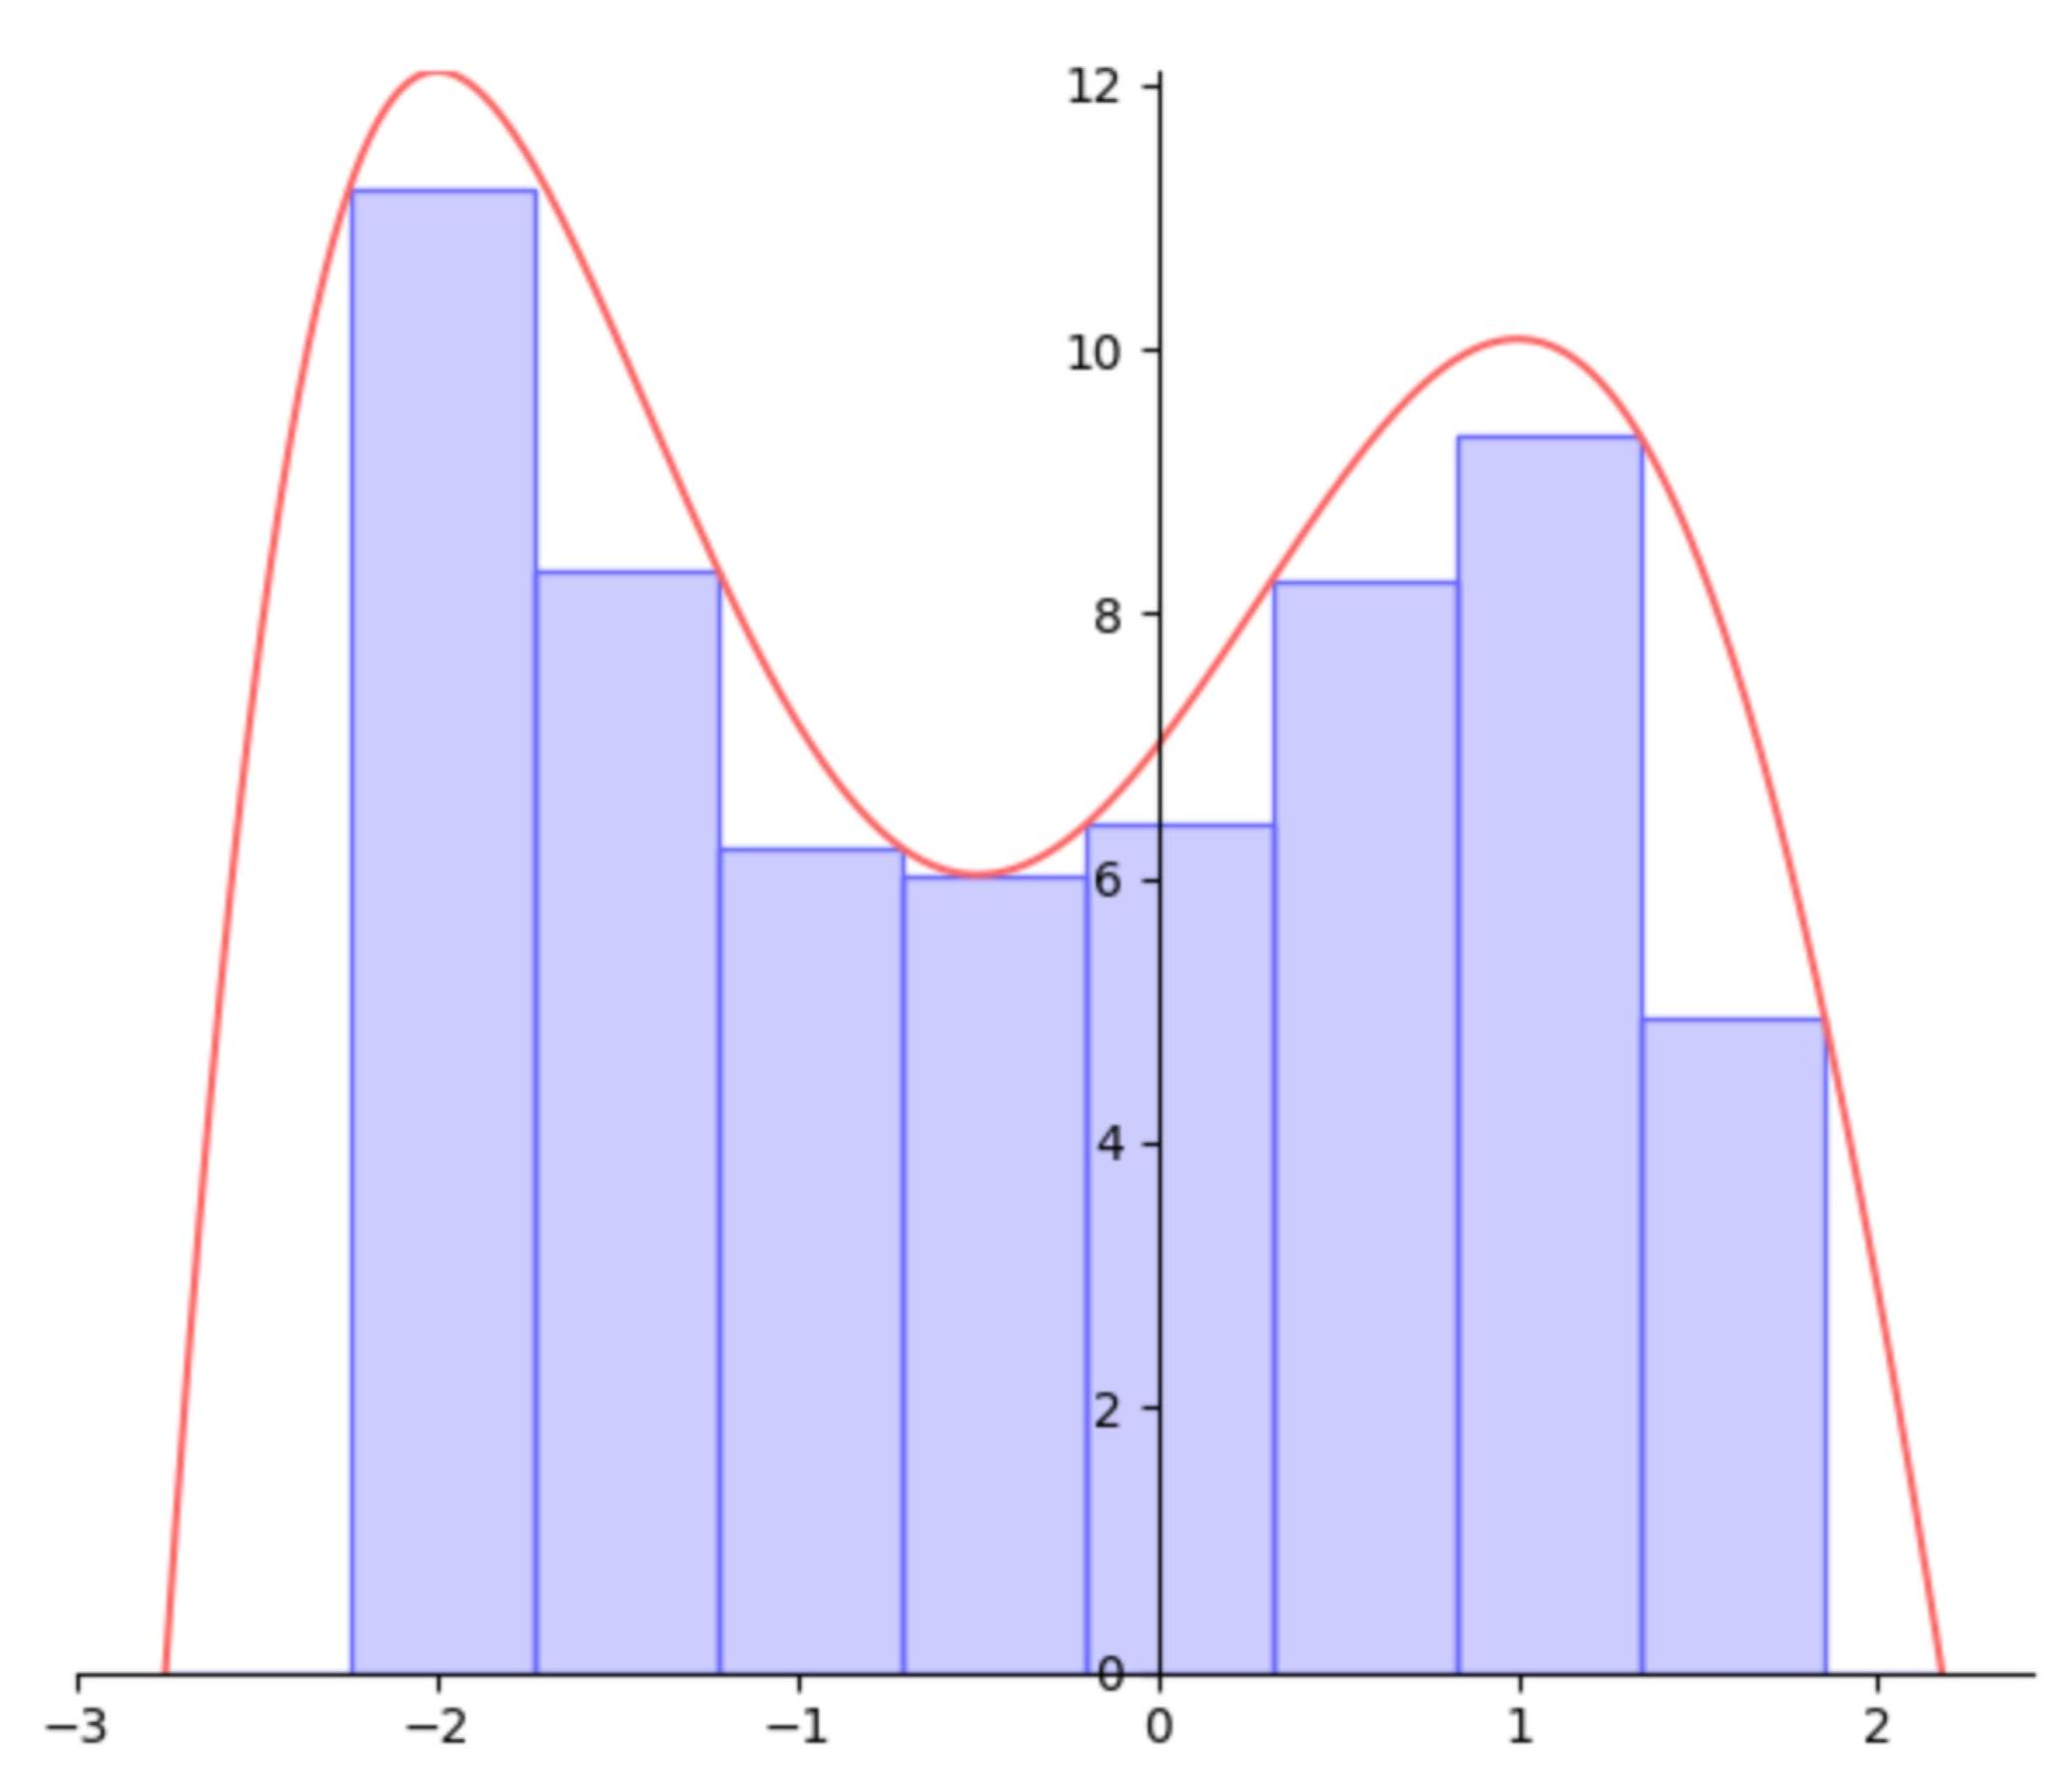
\includegraphics[width=0.4\columnwidth]{figures/nn3.jpg}
%   \vspace{-10pt}
% \end{wrapfigure}

% - ``A NN with sigmoid activation and at most two hidden layers can approximate well a smooth function in $\ell_{1}$-norm"

% - Approx in $\ell_{1}$-norm:
$
\int_{|x| \leq r}\left|f(x)-f_{n}(x)\right| d x \leq \text { Something small }
$


- $f: \mathbb{R} \rightarrow \mathbb{R}$ on a bounded domain, Riemann integrable - its integral can be approximated to any desired accuracy using "lower" and "upper" sums of the area of rectangles

- Approximation of the function by a sum of rectangle functions

$
\int_{|x| \leq r}\left|\color{red}{f(x)}\color{black}-\color{blue}{f_{n}(x)}\color{black}\right| d x 
=\int_{|x| \leq r}\left(\color{red}f(x)\color{black}-\color{blue}f_{n}(x)\color{black}\right) d x 
=\int_{|x| \leq r} \color{red}f(x)\color{black} d x-\int_{|x| \leq r} \color{blue}f_{n}(x) \color{black} d x 
=\int_{|x| \leq r} \color{red}f(x) \color{black}-\color{blue}\sum_{i} \text { Area(Rectangle }_{i})
$


\subsection*{Approximation of the rectangle}


- A rectangle function is equal to the sum of two step functions

- Approximate a step function with a sigmoid
$
\tilde{\phi}(x)=\phi(w(x-b))
$, 
% $b$ where the transition happens, $w$ makes the transition steeper


% Derivative: $\tilde{\phi}^{\prime}(b)=w / 4$
% $\Rightarrow$ The width of the transition is $O(4 / w)$

% $
% h(\phi(w(x-a))-\phi(w(x-b)))
% $


% \subsection*{Conclusion in the 1D case}
% \begin{enumerate}
%   \item Approximate the function in the Riemann sense by a sum of $k$ rectangles

%   \item Represent each rectangle using two nodes in the hidden layer of a neural network

%   \item Compute the sum of all nodes in the hidden layer (considering appropriate weights and signs) to get the final output

% \end{enumerate}

$\Rightarrow \mathrm{NN}$ with one hidden layer containing $2 k$ nodes for a Riemann sum with $k$ rectangles

% - Remarks:

% \begin{itemize}
%   \item The same intuition applies to any sigmoid-like function
%   \item This is an intuitive explanation, not a quantitative one
%   \item The weights $w$ must be large
% \end{itemize}


\subsection*{Larger dimension: $d=2$, same idea}
% Same idea:

% \begin{itemize}
%   \item Approximate the function by $2 \mathrm{D}$ rectangle functions
%   \item Approximate a 2D rectangle function by sigmoids
% \end{itemize}

- Two sigmoids can approximate an infinite rectangle function
% $\left(x_{1}, x_{2}\right) \mapsto \phi\left(w\left(x_{1}-a_{1}\right)\right)-\phi\left(w\left(x_{1}-b_{1}\right)\right)$

% The rectangle:

% \begin{itemize}
%   \item ranges from $a_{1}$ to $b_{1}$ in the $x_{1}$ direction
%   \item is unbounded in the $x_{2}$ direction

% \end{itemize}

% \subsection*{Two sigmoids can approximate an infinite rectangle function}
% $\left(x_{1}, x_{2}\right) \mapsto \phi\left(w\left(x_{2}-a_{2}\right)\right)-\phi\left(w\left(x_{2}-b_{2}\right)\right)$

% The rectangle:

% \begin{itemize}
%   \item ranges from $a_{2}$ to $b_{2}$ in the $x_{2}$ direction
%   \item is unbounded in the $x_{1}$ direction

% \end{itemize}
- Four sigmoids approximate a cross
% \subsection*{Four sigmoids approximate a cross}
% $\left(x_{1}, x_{2}\right) \mapsto \phi\left(w\left(x_{1}-a_{1}\right)\right)-\phi\left(w\left(x_{1}-b_{1}\right)\right)+\phi\left(w\left(x_{2}-a_{2}\right)\right)-\phi\left(w\left(x_{2}-b_{2}\right)\right)$

% $\Rightarrow$ This approximation is close to our objective, with the exception of the two infinite "arms"


% % How can we eliminate the crossed arms?

% \subsection*{Using the sigmoid to threshold unwanted infinite arms}
% Thresholding the function will eliminate the arms

% It is equivalent to composing it with $1_{y \geq c}$ for $c \in(1,2]$

% $\Rightarrow$ Approximate $1_{y \geq c}$ using a sigmoid with a large weight $w$ and an appropriate bias (e.g., $3 w / 2$ )


\subsection*{Point-wise approximations}
- Def: piecewise linear (PWL) function:

$
q(x)=\sum_{i=1}^{m}\left(a_{i} x+b_{i}\right) 1_{r_{i-1} \leq x<r_{i}} \text { with } a_{i} r_{i}+b_{i}=a_{i+1} r_{i}+b_{i+1}
$

- $\ell_{\infty}$-approximation result: Let $f$ be a continuous function on $[c, d]$. $\forall \ \varepsilon>0 \ \exists \ q \text{ s.t.}
\sup _{x \in[c, d]}|f(x)-q(x)| \leq \varepsilon
$


% \subsection*{Linear combinations of RELUs and PWL functions}
% $
% \sum_{i=1}^{m} \tilde{a}_{i}\left(x-\tilde{b}_{i}\right)_{+} \text {is a piecewise linear function }
% $

% How do we get a new segment with slope $a$ starting at $r>\max _{i}\left(\tilde{b}_{i}\right)$ ?

% Intuition: Get the kink at $r$ by setting $\tilde{b}_{i+1}=r$ and slope by additionally canceling existing slope i.e. $\tilde{a}_{i+1}=a-\sum_{i} \tilde{a}_{i}$


\subsection*{PWL functions can be written as combination of RELU}
- \underline{Claim} 1: Any PWL $q$ can be rewritten as
$
q(x)=\tilde{a}_{1} x+\tilde{b}_{1}+\sum_{i=2}^{m} \tilde{a}_{i}\left(x-\tilde{b}_{i}\right)_{+}
$
where $\tilde{a}_{1}=a_{1}, \tilde{b}_{1}=b_{1}, a_{i}=\sum_{j=1}^{i} \tilde{a}_{i}$ and $\tilde{b}_{i}=r_{i-1}$

- \underline{Claim} 2: $q$ can be implemented as a one-hidden-layer NN with RELU activation. Each term corresponds to one node:

% \begin{itemize}
%   \item Bias $-\tilde{b}_{i}$
%   \item Output weight $\tilde{a}_{i}$
% \end{itemize}

% The term $\tilde{a}_{1} x+\tilde{b}_{1}$ also corresponds to one node:

% \begin{itemize}
%   \item Bias $\tilde{b}_{1}$ : bias of the output node
% \end{itemize}



% \begin{itemize}
%   \item Term $\tilde{a}_{1} x=\tilde{a}_{1}(x)_{+}$since $x \in[0,1]$
% \end{itemize}

% \subsection*{\underline{Proof} of the equivalent formulation}

% $
% q(x)=\sum_{i=1}^{m}\left(a_{i} x+b_{i}\right) 1_{r_{i-1} \leq x<r_{i}} \quad r(x)=\tilde{a}_{1} x+\tilde{b}_{1}+\sum_{i=2}^{m} \tilde{a}_{i}\left(x-\tilde{b}_{i}\right)_{+}
% \tilde{a}_{1}=a_{1}, \tilde{b}_{1}=b_{1} \text { , } a_{i}=\sum_{j=1}^{i} \tilde{a}_{j} \text { , } \tilde{b}_{i}=r_{i-1}
% $

% \begin{itemize}
%   \item For $x \in\left[0, r_{1}\right]$
% \end{itemize}

% $
% \left(\tilde{a}_{1}, \tilde{b}_{1}\right)=\left(a_{1}, b_{1}\right) \Longrightarrow q(x)=a_{1} x+b_{1}=\tilde{a}_{1} x+\tilde{b}_{1}=r(x) \text { because } \tilde{b}_{2}=r_{1}
% $

% \begin{itemize}
%   \item For $x \in\left[r_{1}, r_{2}\right], r(x)=\tilde{a}_{1} x+\tilde{b}_{1}+\left(a_{2}-a_{1}\right)\left(x-r_{1}\right)_{+}$
% \end{itemize}

% $
% =a_{1} x+b_{1}+\left(a_{2}-a_{1}\right)\left(x-r_{1}\right)=a_{2} x+b_{1}-\left(a_{2}-a_{1}\right) r_{1}
% $

% $r^{\prime}(x)=a_{2}$ and $r\left(r_{1}\right)=q\left(r_{1}\right)$ as shown above

% $\Longrightarrow r(x)=q(x)$ for $x \in\left[r_{1}, r_{2}\right]$

% \subsection*{\underline{Proof} by induction}
% Let's assume that $r(x)=q(x)$ for $x \in\left[0, r_{i-1}\right]$

% For $x \in\left[r_{i-1}, r_{i}\right]$

% $
% \begin{aligned}
% r(x) & =\tilde{a}_{1} x+\tilde{b}_{1}+\sum_{j=2}^{m} \tilde{a}_{j}\left(x-\tilde{b}_{j}\right)_{+} \\
% & =\tilde{a}_{1} x+\tilde{b}_{1}+\sum_{j=2}^{i} \tilde{a}_{j}\left(x-\tilde{b}_{j}\right) \\
% & =\sum_{j=1}^{i} \tilde{a}_{j} x+\tilde{b}_{1}-\sum_{j=2}^{j} \tilde{a}_{j} \tilde{b}_{j}
% \end{aligned}
% $

% Thus

% \begin{itemize}
%   \item $r^{\prime}(x)=\sum_{j=1}^{i} \tilde{a}_{j}=a_{i}$ good slope
%   \item $r\left(r_{i-1}\right)=q\left(r_{i-1}\right)$ good starting point
% \end{itemize}



% $
% \Longrightarrow r(x)=q(x) \text { for } x \in\left[r_{i-1}, r_{1}\right]
% $

% Why: two affine functions with the same starting point and the same slope are equal

% \subsection*{Recap}
% \begin{itemize}
%   \item Neural networks consist of linear layers stacked together with non-linearities

%   \item A neural network can be seen as a learned feature extractor + a linear predictor

%   \item Neural networks typically require large amounts of data and compute to learn good features

%   \item Neural networks have very high representational power (i.e., the universal approximation result) in contrast to simple models like linear regression

% \end{itemize}
\sectiondivider

\sectionnewcolor

\section{Neural Network Training}

% \subsection*{Training of NNs with SGD}
% - SGD algorithm: Uniformly sample $n$, compute the gradient of $\mathscr{L}_{n}=\frac{1}{2}\left(y_{n}-f\left(x_{n}\right)\right)^{2}$ to update:

% $
% \left(w_{i, j}^{(l)}\right)_{t+1}=\left(w_{i, j}^{(l)}\right)_{t}-\gamma \frac{\partial \mathscr{L}_{n}}{\partial w_{i, j}^{(l)}}\quad\left(b_{i}^{(l)}\right)_{t+1}=\left(b_{i}^{(l)}\right)_{t}-\gamma \frac{\partial \mathscr{L}_{n}}{\partial b_{i}^{(l)}}
% $

% - In Practice: Step size schedule, mini-batch, momentum, Adam

% - Problem: With $O\left(K^{2} L\right)$ parameters, applying chain-rules independently is inefficient due to the compositional structure of $f$

% - Solution: the Backpropagation algorithm computes gradients via the chain rule but reuses intermediate computations

% \subsection*{Description of NN parameters}

$\mathbf{W}^{(1)} \in \mathbb{R}^{d \times K}$, $\mathbf{W}^{(l)} \in \mathbb{R}^{K \times K}$ for $2 \leq l \leq L$, $\mathbf{W}^{(L+1)} \in \mathbb{R}^{K}$, $b^{(l)} \in \mathbb{R}^{K}$ for $1 \leq l \leq L$, $b^{(L+1)} \in \mathbb{R}$

\subsection*{Compact description of output}

\begin{itemize}
  % \item $x^{(1)}=f^{(1)}\left(x^{(0)}\right):=\phi\left(\left(\mathbf{W}^{(1)}\right)^{\top} x^{(0)}+b^{(1)}\right)$
  \item $x^{(l)}=f^{(l)}\left(x^{(l-1)}\right):=\phi\left(\left(\mathbf{W}^{(l)}\right)^{\top} x^{(l-1)}+b^{(l)}\right)$
  \item $y=f^{(L+1)}\left(x^{(L)}\right):=\left(\mathbf{W}^{(L+1)}\right)^{\top} x^{(L)}+b^{(L+1)}$
\end{itemize}

% The overall function $y=f\left(x^{(0)}\right)$ is just the composition of the layer functions:

$
f=f^{(L+1)} \circ f^{(L)} \circ \cdots \circ f^{(l)} \circ \cdots \circ f^{(2)} \circ f^{(1)}
$

% - Cost function:
$
\mathscr{L}=\frac{1}{2 N} \sum_{n=1}^{N}\left(y_{n}-f^{(L+1)} \circ \cdots \circ f^{(2)} \circ f^{(1)}\left(x_{n}\right)\right)^{2}
$

% - Remarks:

% \begin{itemize}
%   \item The specific form of the loss is not crucial
%   \item $\mathscr{L}$ is a function of all weight matrices and bias vectors
%   \item Each function $f^{(l)}$ is parameterized by weights $\mathbf{W}^{(l)}$ and biases $b^{(l)}$
% \end{itemize}

% \subsection*{Chain rule}

% $
% \mathscr{L}_{n}=\frac{1}{2}\left(y_{n}-f^{(L+1)} \circ \cdots \circ f^{(l+1)} \circ \phi(\underbrace{\left.\left(\mathbf{W}^{(l)}\right)^{\top} x^{(l-1)}+b^{(l)}\right)}_{z^{(l)}})\right)^{2}
% $



% $
% \frac{\partial \mathscr{L}_{n}}{\partial w_{i, j}^{(l)}} \quad ?
% $

\subsection*{Chain rule}
$
\mathscr{L}_{n}=\frac{1}{2}\left(y_{n}-f^{(L+1)} \circ \cdots \circ f^{(l+1)} \circ \phi\left(z^{(l)}\right)\right)^{2}
$

% \includegraphics*[width=\columnwidth]{figures/nn4.png}

$
\frac{\partial \mathscr{L}_{n}}{\partial w_{i, j}^{(l)}} =\sum_{k=1}^{K} \frac{\partial \mathscr{L}_{n}}{\partial z_{k}^{(l)}} \frac{\partial z_{k}^{(l)}}{\partial w_{i, j}^{(l)}}
=\frac{\partial \mathscr{L}_{n}}{\partial z_{j}^{(l)}} \frac{\partial z_{j}^{(l)}}{\partial w_{i, j}^{(l)}} 
=\frac{\partial \mathscr{L}_{n}}{\partial z_{j}^{(l)}} \cdot x_{i}^{(l-1)}
\text { since } \frac{\partial z_{k}^{(l)}}{\partial w_{i, j}^{(l)}}=0 \text { for } k \neq j,
\text { since } z_{j}^{(l)}=\sum_{k=1}^{K} w_{k, j}^{(l)} x_{k}^{(l-1)}+b_{j}^{(l)}
$

% We need to compute $\frac{\partial \mathscr{L}_{n}}{\partial z_{j}^{(l)}}, z^{(l)}, x_{i}^{(l-1)}$ and reuse them for different $\frac{\partial \mathscr{L}_{n}}{\partial w_{i, j}^{(l)}}$

% \subsection*{Forward Pass}
% $
% x^{(0)}=x_{n} \in \mathbb{R}^{d}
% z^{(l)}=\left(\mathbf{W}^{(l)}\right)^{\top} x^{(l-1)}+b^{(l)} \ , \
% x^{(l)}=\phi\left(z^{(l)}\right)
% $

% Computational complexity $\Rightarrow$ $O\left(K^{2} L\right)$

% \subsection*{Backward pass (I)}
% Define $\delta_{j}^{(l)}=\frac{\partial \mathscr{L}_{n}}{\partial z_{j}^{(l)}}=\sum_{k} \frac{\partial \mathscr{L}_{n}}{\partial z_{k}^{(l+1)}} \frac{\partial z_{k}^{(l+1)}}{\partial z_{j}^{(l)}}=\sum_{k} \delta_{k}^{(l+1)} \frac{\partial z_{k}^{(l+1)}}{\partial z_{j}^{(l)}}
% $

% \subsection*{Backward pass (II)}
% - Using $z_{k}^{(l+1)}=\sum_{i=1}^{K} w_{i, k}^{(l+1)} x_{i}^{(l)}+b_{k}^{(l+1)}=\sum_{i=1}^{K} w_{i, k}^{(l+1)} \phi\left(z_{i}^{(l)}\right)+b_{k}^{(l+1)}$

% - We obtain $\frac{\partial z_{k}^{(l+1)}}{\partial z_{j}^{(l)}}=\phi^{\prime}\left(z_{j}^{(l)}\right) w_{j, k}^{(l+1)}$

% - Thus
% $
% \delta_{j}^{(l)}=\sum_{k} \delta_{k}^{(l+1)} \phi^{\prime}\left(z_{j}^{(l)}\right) w_{j, k}^{(l+1)}
% $

% $
% \delta^{(l)}=\left(\mathbf{W}^{(l+1)} \delta^{(l+1)}\right) \odot \phi^{\prime}\left(z^{(l)}\right)
% $

% \subsection*{Backward pass (III)}
% Initialization (first derivative):

% $
%
% \delta^{(L+1)} =\frac{\partial}{\partial z^{(L+1)}} \frac{1}{2}\left(y_{n}-z^{(L+1)}\right)^{2}
% =z^{(L+1)}-y_{n}
%
% $

% $
% \delta^{(l)}=\left(\mathbf{W}^{(l+1)} \delta^{(l+1)}\right) \odot \phi^{\prime}\left(z^{(l)}\right)
% $

% Computational complexity: $O\left(K^{2} L\right)$

\subsection*{Derivatives computation}


- Using $z_{m}^{(l)}=\sum_{k=1}^{K} w_{k, m}^{(l)} x_{k}^{(l-1)}+b_{m}^{(l)}$ :

$\frac{\partial \mathscr{L}_{n}}{\partial b_{j}^{(l)}}=\sum_{k=1}^{K} \frac{\partial \mathscr{L}_{n}}{\partial z_{k}^{(l)}} \frac{\partial z_{k}^{(l)}}{\partial b_{j}^{(l)}}=\frac{\partial \mathscr{L}_{n}}{\partial z_{j}^{(l)}} \frac{\partial z_{j}^{(l)}}{\partial b_{j}^{(l)}}=\delta_{j}^{(l)}$

$\frac{\partial \mathscr{L}_{n}}{\partial w_{i, j}^{(l)}}=\sum_{k=1}^{K} \frac{\partial \mathscr{L}_{n}}{\partial z_{k}^{(l)}} \frac{\partial z_{k}^{(l)}}{\partial w_{i, j}^{(l)}}=\frac{\partial \mathscr{L}_{n}}{\partial z_{j}^{(l)}} \frac{\partial z_{j}^{(l)}}{\partial w_{i, j}^{(l)}} =\delta_{j}^{(l)} \cdot x_{i}^{(l-1)}$

\subsection*{Backpropagation algorithm}
Forward pass $\mathcal{O}\left(K^{2} L\right)$:

$
x^{(0)}=x_{n} \in \mathbb{R}^{d},
z^{(l)}=\left(\mathbf{W}^{(l)}\right)^{\top} x^{(l-1)}+b^{(l)},
x^{(l)}=\phi\left(z^{(l)}\right)
$

Backward pass $\mathcal{O}\left(K^{2} L\right)$:

$
\delta^{(L+1)}=z^{(L+1)}-y_{n},
\delta^{(l)}=\left(\mathbf{W}^{(l+1)} \delta^{(l+1)}\right) \odot \phi^{\prime}\left(z^{(l)}\right)
$



Compute the derivatives:
$
\frac{\partial \mathscr{L}_{n}}{\partial w_{i, j}^{(l)}}=\delta_{j}^{(l)} x_{i}^{(l-1)},
\frac{\partial \mathscr{L}_{n}}{\partial b_{j}^{(l)}}=\delta_{j}^{(l)}
$

% \subsection*{Parameter Initialization}
% \begin{itemize}
%   \item In deep networks, improper parameter initialization can lead to the vanishing or exploding gradients problem

%   \item Problem: Extremely slow or unstable optimization

%   \item Solution: Control the layerwise variance of neurons (aka He initialization)

% \end{itemize}

% \subsection*{Variance-Preserving Initialization}
% - for ReLU networks:

% \begin{itemize}
%   \item $z^{(l)} \sim \mathcal{N}\left(0, \mathbf{I}_{K}\right)$ : pre-activations at layer $l$ ($\operatorname{Var}\left[z_{i}^{(l)}\right]=1$ )

%   \item $w_{i}^{(l+1)} \sim \mathcal{N}\left(0, \sigma \mathbf{I}_{K}\right)$ : the $i$-th weight vector at layer $l+1$

%   \item $z_{i}^{(l+1)}=\operatorname{ReLU}\left(z^{(l)}\right)^{\top} w_{i}^{(l+1)}$
%   \item We set $\sigma=\sqrt{2 / K}$ so that $\operatorname{Var}\left[z_{i}^{(l+1)}\right]=1$

% \end{itemize}


\subsection*{Batch Normalization}
% - Batch $B=\left(x_{1}, \cdots, x_{M}\right)$ and denote by $z_{n}^{(l)}$ the layer's pre-activation input corresponding to the observation $x_{n}$

% - Step 1: Normalize each layer's input using its mean and its variance over the batch:
$
\bar{z}_{n}^{(l)}=\frac{z_{n}^{(l)}-\mu_{B}^{(l)}}{\sqrt{\left(\sigma_{B}^{(l)}\right)^{2}+\varepsilon}}
$ (Component-wise)
where $\mu_{B}^{(l)}=\frac{1}{M} \sum_{n=1}^{M} z_{n}^{(l)}$ and $\left(\sigma_{B}^{(l)}\right)^{2}=\frac{1}{M} \sum_{n=1}^{M}\left(z_{n}^{(l)}-\mu_{B}^{(l)}\right)^{2}$, and $\varepsilon \in \mathbb{R}_{\geq 0}$ is a small value added for numerical stability

- Introduce learnable parameters $\gamma^{(l)}, \beta^{(l)} \in \mathbb{R}^{K}$ to reverse the normalization :
$
\hat{z}_{n}^{(l)}=\gamma^{(l)} \odot \bar{z}_{n}^{(l)}+\beta^{(l)}
$

- Scale-invariance: 
% For $\varepsilon \approx 0$, the output is invariant to activation-wise affine scaling of $z_{n}^{(l)}$
$
\mathrm{BN}\left(a \odot z_{n}^{(l)}+b\right)=\mathrm{BN}\left(z_{n}^{(l)}\right) 
$
% $\text { for } a \in \mathbb{R}_{>0}^{K} \text { and } b \in \mathbb{R}^{K}$
% e.g. $\Rightarrow$ no need to include a bias before BatchNorm.

- Inference: Estimate $\hat{\mu}^{(l)}=\mathbf{E}\left[\mu_{B}^{(l)}\right]$ and $\hat{\sigma}^{(l)}=\mathbf{E}\left[\sigma_{B}^{(l)}\right]$ during training, use these for inference

\subsection*{Layer Normalization}
% - Step 1: Normalize each layer's input using its mean and its variance over the features (instead of over the inputs):
$
\bar{z}_{n}^{(l)}=\frac{z_{n}^{(l)}-\mu_{n}^{(l)} \cdot 1_{K}}{\sqrt{\left(\sigma_{n}^{(l)}\right)^{2}+\varepsilon}}
$
where $\mu_{n}^{(l)}=\frac{1}{K} \sum_{k=1}^{K} z_{n}^{(l)}(k)$ and $\left(\sigma_{n}^{(l)}\right)^{2}=\frac{1}{K} \sum_{k=1}^{K}\left(z_{n}^{(l)}(k)-\mu_{n}^{(l)}\right)^{2}$, and $\varepsilon \in \mathbb{R}_{\geq 0}$

- Learnable parameters $\gamma^{(l)}, \beta^{(l)} \in \mathbb{R}^{K}$ :
$
\hat{z}_{n}^{(l)}=\gamma^{(l)} \odot \bar{z}_{n}^{(l)}+\beta^{(l)}
$

\begin{itemize}
  \item Normalize across features, independently for each observation
  \item common alternative, widely used for transformers and text data
  \item No batch dependency, use the same for training and inference
\end{itemize}

% \subsection*{Normalization Benefits}

% \begin{itemize}
%   \item Stabilizes activation magnitudes / reduces initialization impact
%   \item Additional regularization effect from noisy $\mu_{B}^{(l)}, \sigma_{B}^{(l)}$ in batch norm
%   \item Stabilizes and speeds up training, allows larger learning rates
%   \item Used in almost all modern deep learning architectures
%   \item Often inserted after every convolutional layer, before non-linearity
% \end{itemize}

% \subsection*{Recap}
% \begin{itemize}
%   \item Neural networks are trained with gradient-based methods such as SGD

%   \item To compute the gradients, we use backpropagation, which involves the chain rule to efficiently calculate the gradients based on the network's intermediate outputs $z^{(l)}$ and $\delta^{(l)}$

%   \item Proper parameter initialization should avoid exploding and vanishing gradients by carefully controlling the layerwise variance

%   \item Batch and Layer normalization dynamically stabilize the training process, allowing for faster convergence and the use of larger learning rates

% \end{itemize}
\sectiondivider

\sectionnewcolor
\section*{Convolutional Networks}
\subsection*{CNN General Structure}


\begin{itemize}
  \item Convolutional networks consist of sparsely connected convolutional layers in place of fully-connected linear layers
  \item Pooling layers perform spatial downsampling (typically typically reducing the dimensions from $H \times W$ to $H / 2 \times W / 2$
  \item A fully-connected network at the end performs classification based on the extracted features
\end{itemize}


\begin{itemize}
  \item Fully connected NNs have $O\left(K^{2} L\right)$ parameters: training requires a lot of data
  \item Fully connected neural networks interpret an image as a flattened vector, disregarding the original spatial dependencies
\end{itemize}


\subsection*{Convolution}
$
x_{n, m}^{(1)}=\sum_{k, l} f_{k, l} \cdot x_{n-k, m-l}^{(0)}
$

\begin{itemize}
  \item We consider local filters: $f_{k, l} \neq 0$ for small values of $|k|$ and $|l|$
\end{itemize}

$\rightarrow x_{n, m}^{(1)}$ only depends on the value of $x^{(0)}$ close to $(n, m)$

$\rightarrow f$ represents the learnable weights

\begin{itemize}
  \item We use the same filter at every position - weight sharing

  \item Translation equivariance - a shifted input results in a shifted output
  \item  Convolution requires fewer parameters which are universal across different locations

\end{itemize}


\subsection*{Handling of borders}
- Zero padding: Add zeros to each side of the input's boundaries $\Rightarrow$ same dimension as the input

- Valid padding: Perform the convolution only where the entire filter fits inside the original data $\Rightarrow$ smaller dimensions than the input

\subsection*{Filter for Multi-Channel Convolution}

\begin{itemize}
  \item For multi-channel inputs, the filter has the same number of channels as the input
  \item The filter channels and the bias are the learnable parameters of the filter
\end{itemize}

\subsection*{Multi-Channel Output from Multiple Filters}
- It is common to use multiple filters. Each filter processes the input to produce a separate channel

- Applying different filters to an input generates multiple output channels.

\subsection*{Convolutional Layer}

\begin{wrapfigure}{r}{0.5\columnwidth} 
    \centering
    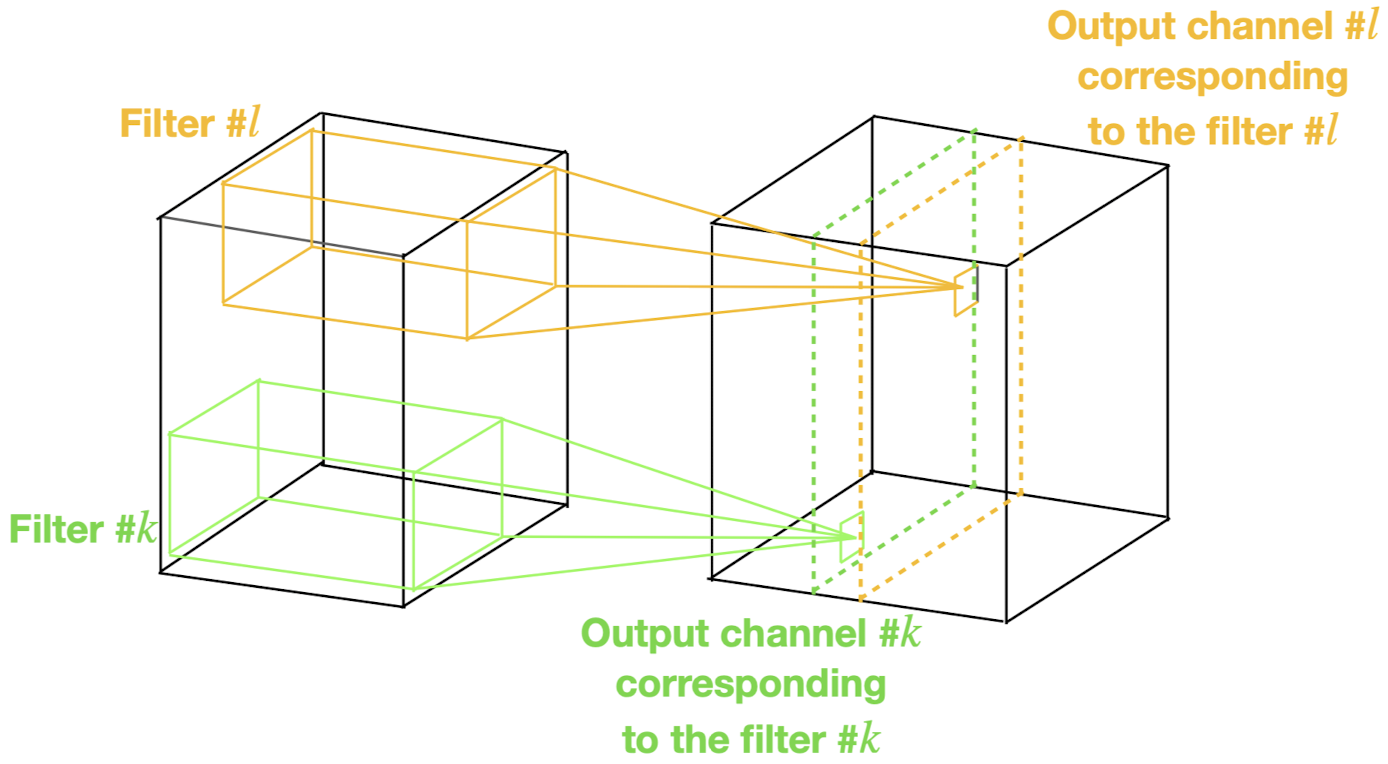
\includegraphics[width=0.5\columnwidth]{figures/conv_layer.png}
    \vspace{-10pt}
\end{wrapfigure}

- A convolutional layer is composed of multiple filters

- Each output channel corresponds to its own independent filter

- Hyper-parameters of the convolutional layer: size, padding, stride


\subsection*{Pooling}
- often applied after the convolutional layer

- Max pooling: returns the maximum value of the portion of the convolved feature that is covered by the kernel

- Average pooling: returns the average value of the portion of the convolved feature that is covered by the kernel

- Pooling is a downsampling operation that reduces the spatial dimensions of the convolved feature

- Remark: Pooling layers do not have learnable parameters 

- Hyperparameters are the size, type, and stride of the pooling operation

\subsection*{Non-linearity and CNNs}

- Important: A non-linearity such as ReLU is included after each convolutional layer to make the model non-linear

\subsection*{CNNs: General Structure}
\includegraphics*[width=\columnwidth]{figures/CNN.jpg}

- Depth: $\uparrow$ \# channels, $\downarrow$ dimensions

- Receptive field (area of input that affects a given neuron) increases with depth:

\begin{itemize}
  \item First layers extract low-level features, e.g., edges, colors ($\downarrow$ receptive field + $\downarrow$ depth)
  \item Subsequent layers extract high-level features, e.g., objects ($\uparrow$ receptive field + $\uparrow$ depth)
\end{itemize}

- ConvNet reduces the images to a form easier to process without losing essential features

\subsection*{Backpropagation with weight sharing}
- Weight sharing is used in CNN: many edges use the same weights

\underline{Training:}

\begin{enumerate}
  \item Run backpropagation as if the weights were not shared (treat each weight as an independent variable)

  \item Once the gradient is computed, sum the gradients of all edges that share the same weight

\end{enumerate}

Let $f(x, y, z): \mathbb{R}^{3} \rightarrow \mathbb{R}$ and $g(x, y)=f(x, y, x)$

$
(\frac{\partial g}{\partial x}(x, y), \frac{\partial g}{\partial y}(x, y)) \\\underset{\text {Chain rule }}{=}(\frac{\partial f}{\partial x}(x, y, x)+\frac{\partial f}{\partial z}(x, y, x), \frac{\partial f}{\partial y}(x, y, x))
$

\subsection*{Learned Convolutional Filters}

- Edge and color detectors typically emerge when trained on large datasets

- Individual Activations Can Be Interpretable

- Activations in later layers detect more complex patterns

\subsection*{Residual Networks}
\subsection*{Skip Connections and Residuals}
\begin{itemize}
  \item Starting point: Adding more layers should lead to the same or lower training loss as they can learn the identity function

  \item ResNet paper indicates that this is not always the case

  \item Solution: add a skip connection around some layers $F(\mathbf{X})$

  \item Standard network: $\mathbf{Y}=F(\mathbf{X})$

  \item Residual network: $\mathbf{Y}=R(\mathbf{X})+\mathbf{X}$ where $R(\mathbf{X})$ is called a residual branch


  \item Technical detail: If $\operatorname{size}(\mathbf{Y}) \neq \operatorname{size}(\mathbf{X})$, additional operations are needed on the skip connection to match the dimensions

  \item Skip connections address the observed convergence issue, making the training of very deep networks (with hundreds of layers) feasible

  \item Skip connections are used in almost all modern neural networks (including CNNs and transformers)

\end{itemize}


\subsection*{Popular architectures}

VGG \& ResNet


\subsection*{Data Augmentation}
- Generate new data from the data

- Note dangers of excessive augmentation (e.g. rotation on MNIST)!

- Transformation $\tau: \mathbb{R}^{d} \rightarrow \mathbb{R}^{d}$ which preserves the labels (i.e., $y_{x}=y_{\tau(x)}$ )

$
S=S_{\text {train }} \cup\left\{\left(\tau\left(x_{i}\right), y_{i}\right)\right\}_{i=1}^{n}
$

\begin{itemize}
  \item We train on more data

  \item Encourages models to be invariant to $\tau$

  \item It can be seen as regularization

  \item These transformations are task and dataset specific

\end{itemize}

- Pictures can also be cropped, resized, or perturbed by a small amount of noise



\subsection*{Weight Decay: $l_{2}$-regularization}

- Regularize weights without regularizing bias terms:
$
\min \mathscr{L}+\frac{\lambda}{2} \sum_{l}\left\|\mathbf{W}^{(l)}\right\|_{F}^{2}
$

- Favors small weights which can aid in generalization and optimization

- Optimization with gradient descent:

$
\left(w_{i, j}^{(l)}\right)_{t+1}=\left(w_{i, j}^{(l)}\right)_{t}-\eta \nabla \mathscr{L}-\eta \lambda\left(w_{i, j}^{(l)}\right)_{t}=\underbrace{(1-\eta \lambda)}_{\text {weight decay }}\left(w_{i, j}^{(l)}\right)_{t}-\eta \nabla \mathscr{L}
$

- Interaction with BatchNorm:

\begin{itemize}
  \item $\mathrm{BN}(\mathbf{W X})=\mathrm{BN}(\alpha \mathbf{W X})$ for $\alpha \in \mathbb{R}_{>0}$ (assuming $\varepsilon \approx 0$ )
  \item $\mathrm{BN}$ is scale invariant in $\mathbf{W}$, hence there is no direct regularization effect from WD
  \item However, the training dynamics differ 
\end{itemize}


\subsection*{Dropout: randomly drop nodes}
- Def: At each training step, retain with probability $p^{(l)}$ each node in layer $(l)$ :

- We drop nodes independently for each element of a mini-batch

- Training phase: Run one step of SGD on the subnetwork and update the weights

- Testing phase: 

\begin{itemize}
    \item Use all nodes
  \item Scale each of them by the factor $p^{(l)}$ to ensure that the expected output (when considering the probability of dropping nodes during training) matches the actual output at test time
\end{itemize}

- Remark: Weight rescaling can be implemented during training time by scaling the weights by $1 / p^{(l)}$ after each weight update - how it is implemented in practice

- Note: Variance is generally not preserved and as a result Dropout often works poorly with normalization

\subsection*{Dropout: results}
\begin{itemize}
  \item Setting: Fully-connected networks of different width and depth on MNIST

  \item Dropout results in lower test error

  \item However, dropout typically requires more iterations to converge due to increased stochastic noise

\end{itemize}


\subsection*{Recap}
\begin{itemize}
  \item Convolutional networks are composed of sparsely connected convolutional layers instead of fully-connected linear layers

  \item The same convolution is applied as a sliding window across all spatial locations

  \item Data augmentation usually results in a significant improvement in the model's generalization performance

  \item Weight decay and dropout can further enhance the performance, though typically to a lesser extent

\end{itemize}
\sectiondivider

\sectionnewcolor
\section{Transformers}

% - A transformer is a neural network that iteratively transforms a sequence to another sequence and mixes the information between the sequence elements via self-attention.

% \subsection*{Architecture}


% \begin{wrapfigure}{r}{0.4\columnwidth} 
%     \centering
%     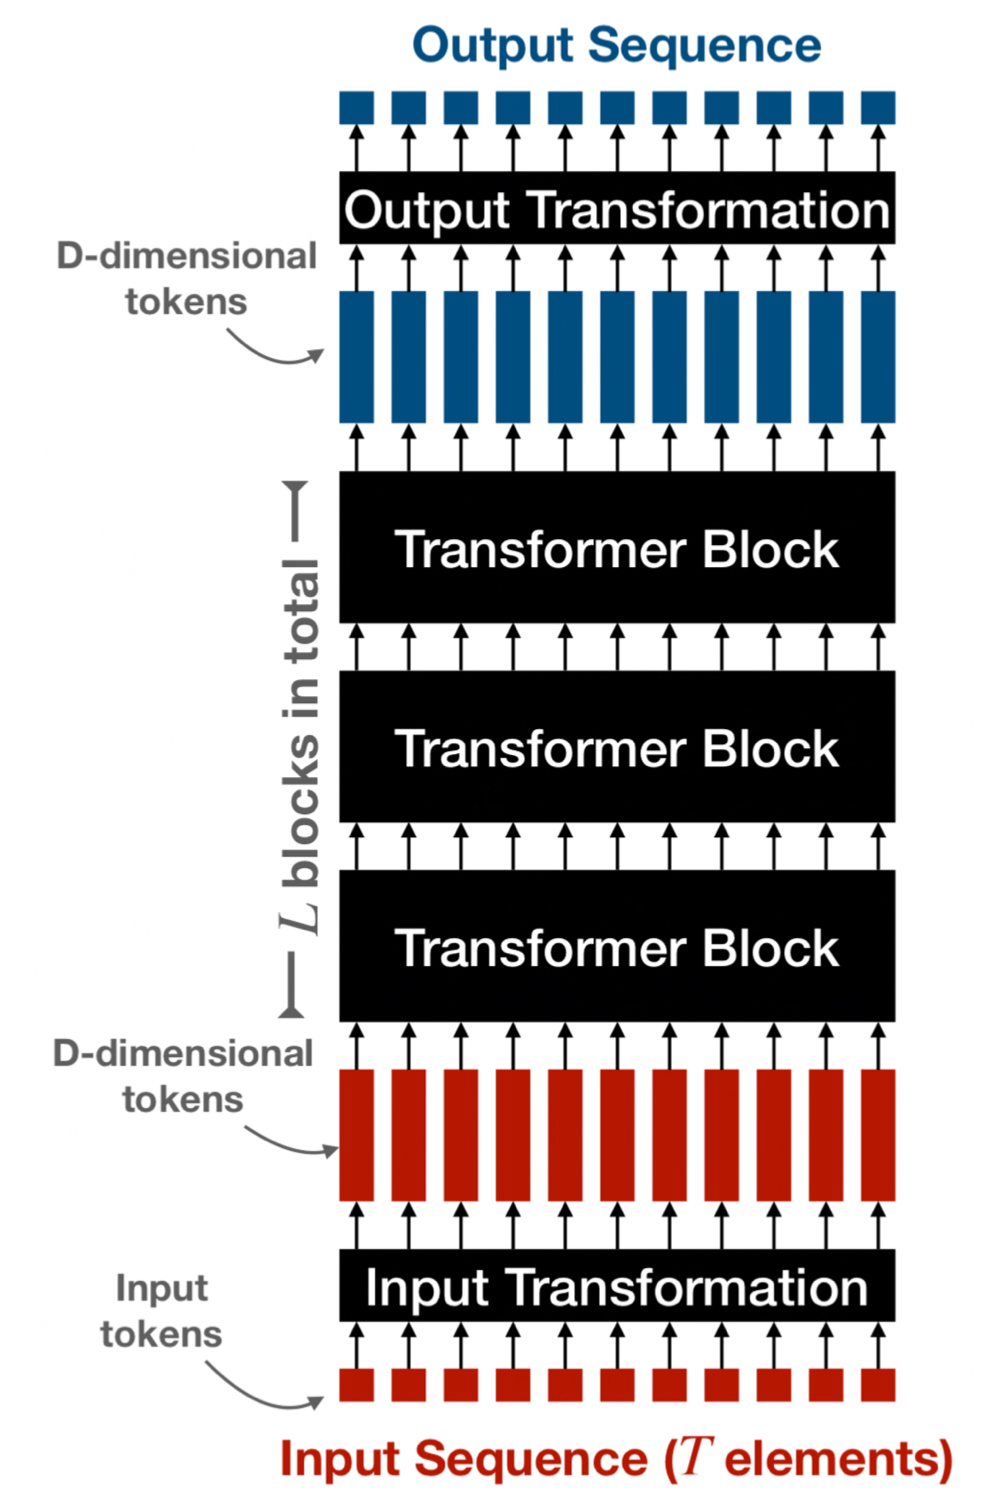
\includegraphics[width=0.4\columnwidth]{figures/transformer_architecture.jpeg}
%     \vspace{-10pt}
% \end{wrapfigure}

- Self-Attention (SA): mixes information between tokens

- Multi-Layer Percep. (MLP): mixes information within each token

- Skip connections are widely used

- Layer normalization (LN) placed at the start of a residual branch

% \begin{wrapfigure}{l}{0.2\columnwidth}
%   % \centering
%   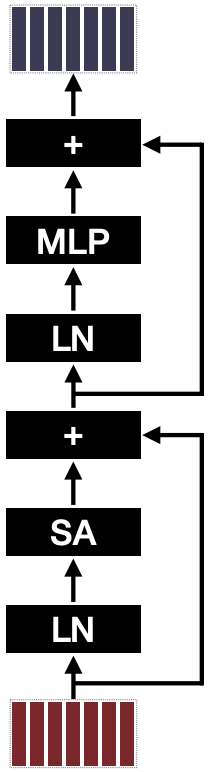
\includegraphics[width=0.2\columnwidth]{figures/transformer_block.png}
% %   \caption{}
% %   \label{fig:cfm_pca2D_wrapped}
% \end{wrapfigure}

\subsection*{Text Token Embeddings}

- Tokenization: split text into sequence of tokens (predefined)

- Convert each token ID $i\in\{1,...,N_{vocab}\}$ into $\mathbf{w}_{i}\in\mathbb{R}^{D}$

- Matrix multiplication $\mathbf{W}\cdot\mathbf{e}_{i}=\mathbf{W}_{:,i}=\mathbf{w}_{i}{\mathrm{~(with~\mathbf{W}\in\mathbb{R}^{D \times N_{vocab}}}})$


- $\mathbf{W}$ learned via backpropagation
% , along with all other transformer parameters (however, the tokenizer procedure is typically fixed in advance and not learned)

- Input sequence of $T$ tokens leads to an input matrix $X\in\mathbb{R}^{T\times D}$

\subsection*{Attention: learning input-dependent weighted average}



% - Attention is a function that transforms a sequence of tokens to a new sequence of tokens using a learned input-dependent weighted average

- Input tokens : $V\in\mathbb{R}^{T_{i n}\times D}$, Output tokens : $Z\in\mathbb{R}^{T_{out}\times D}$

% - Output tokens are simply a weighted average of
% the input tokens:
$z_{i}=\sum_{j=1}^{T_{i}}p_{i j}v_{j}$ i.e. $Z=P V$, Weighting coefficients ${\cal P}\in[0,1]^{T_{out}\times T_{i n}}$ valid probability distributions over input $\textstyle\sum_{j=1}^{T_{i n}}p_{i j}=1$


\begin{wrapfigure}{r}{0.4\columnwidth}
  % \centering
  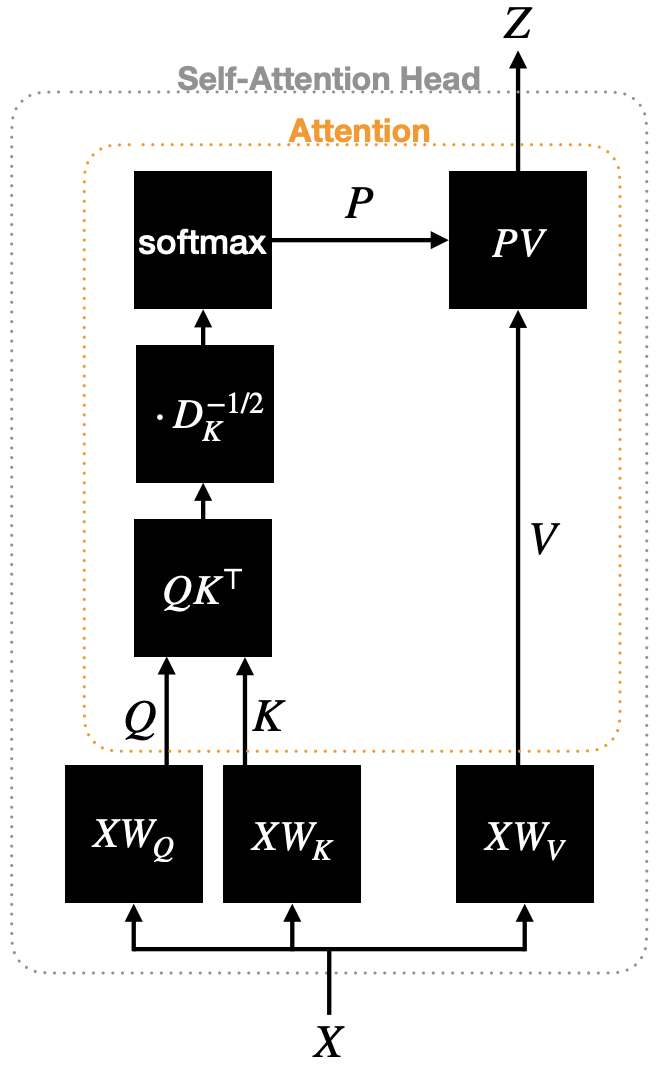
\includegraphics[width=0.4\columnwidth]{figures/self_attention.png}
%   \caption{}
%   \label{fig:cfm_pca2D_wrapped}
\end{wrapfigure}

- Query tokens : $Q\in\mathbb{R}^{T_{out}\times D_{K}}$, Key tokens : $K\in\mathbb{R}^{T_{in}\times D_{K}}$


- Determine weight $p_{i,j}$ based on how simmilar $q_i$ and $k_j$ are.

- Use inner product to obtain raw similarity scores.

- Normalize with softmax (scaled temperature by $\sqrt{D_{K}}$) to obtain a probability distribution. (applied on each row independently)

% - $P=\mathrm{softmax}\left({\frac{Q K^{\mathsf{T}}}{\sqrt{D_{K}}}}\right)$ 
% - The softmax is applied on each row independently. 

- Scaling $\rightarrow$ uniformity at initialization and faster convergence

\subsection*{Self-Attention}



- $V,K,Q$ all derived from same input token
sequence $X\in\mathbb{R}^{T\times D}$

- Values : $V=X W_{V}\in\mathbb{R}^{T\times D},\,W_{V}\in\mathbb{R}^{D\times D}$

- Keys : $K=X W_{K}\in\mathbb{R}^{T\times D_{K}},\,W_{K}\in\mathbb{R}^{D\times D_{K}}$

- Queries : $Q=X W_{Q}\in\mathbb{R}^{T\times D_{K}},W_{Q}\in\mathbb{R}^{D\times D_{K}}$

- $W_{Q},\,W_{V},\,W_{K}$ are learned params.

- $Z=\mathrm{softmax}\left(\frac{X W_{Q}W_{K}^{T}X^{T}}{\sqrt{D_{K}}}\right)X W_{V}$

\subsubsection*{Multi-Head Self-Attention}

% \begin{wrapfigure}{r}{0.3\columnwidth} 
%   \centering
%   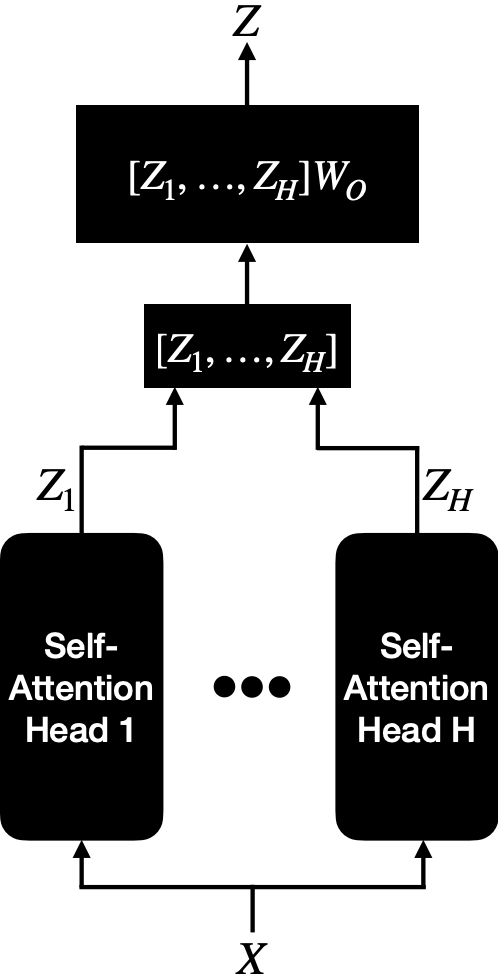
\includegraphics[width=0.3\columnwidth]{figures/multi_head.png}
% \end{wrapfigure}

- Run $H$ Self-Attention “heads” in parallel 
$Z_{h}={\mathrm{softmax}}\left({\frac{X W_{Q,h}W_{K,h}^{\mathsf{T}}X^{\mathsf{T}}}{\sqrt{D_{K}}}}\right)X W_{V,h}\in\mathbb{R}^{T\times D_{V}}$, 
$W_{V,h}\in\mathbb{R}^{D\times D_{V}},\,W_{K,h}\in\mathbb{R}^{D\times D_{K}},\,W_{Q,h}\in\mathbb{R}^{D\times D_{K}}$,
$Z=[Z_{1},\dots,Z_{H}]W_{o}$ where $W_{O}\in\mathbb{R}^{H D_{V}\times D}$ is learned via backprop
% \lipsum[1]

\subsection*{Positional Information}

- Attention by itself does not account for the order of input

- positional encoding in the network $p o s:\left\{1,...,T\right\}\rightarrow\mathbb{R}^{D}$

- e.g. $W_{p o s}$ corresponding to each token's position $t$ to the input embedding. $W_{p o s}\in\mathbb{R}^{D\times T}$ is learned via backprop

\subsection*{MLP: Mixing Information within Tokens}
- Apply the same transformation to each token
independently: $M L P(X)=\varphi(X W_{1})W_{2}$,
$W_{1},W_{2}\in\mathbb{R}^{D\times D}$ learned via backprop

\subsection*{Output Transformations}

% - typically simple: linear transformation or a small MLP

- Single output: transfo. to a special taskspecific input token or to the average tks. Multi outputs: transfo to each token indep.

\subsection*{Vision Transformer Architecture}

% - Self-attention, more general than convolution 

- The receptive field is the whole image after one SA layer

- ViTs require more data than CNNs, reduced inductive bias in extracting local features

- Model attends to image regions semantically relevant for clf

\subsection*{Encoders \& Decoders}

% \begin{wrapfigure}{r}{0.3\columnwidth} 
%   \centering
%   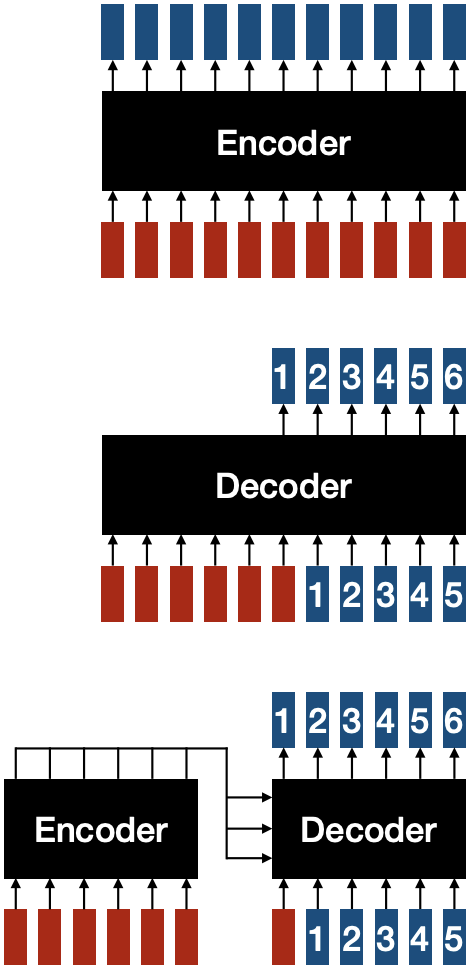
\includegraphics[width=0.3\columnwidth]{figures/encoders_decoders.png}
% \end{wrapfigure}

- Encoders: fixed output size and process all inputs simultaneously

- Decoders: Auto-regressively sample the next token as $x_{t+1}\sim s o f i m a x(f(x_{1},....,x_{t}))$
%  and use it as new input token. Capable of generating responses of arbitrary length.

% - Encoder-decoder (e.g., translation): First encode the whole input (e.g., in one language) and then decode to token by token (e.g., in a different language)

\sectiondivider

\sectionnewcolor
\section*{Adversarial ML}

- We don't understand how NN models generalize and react to shifts in the distribution of data (i.e., distribution shifts)

- Classification problem: $(X,Y)\sim{\mathcal{D}},\;Y$ with range $\{-1,1\}$

- Standard risk: average zero-one loss over $X$: $R(f)=\mathbb{E}_{\mathcal{D}}\left[1_{f(X)\neq Y}\right]=\mathbb{P}_{\mathcal{D}}\left[f(X)\neq Y\right]$ i.e. minimise proba of wrong prediction.


- Adversarial risk: average zero-one loss over small, worst-case perturbations of $X$: $R_{\varepsilon}(f)={{{\mathbb{E}}}}_{\mathcal{D}}\left[\operatorname*{max}_{\hat{x},\|\hat{x}-X\|\leq\varepsilon}1_{f(\hat{x})\neq Y}\right]$

\subsection*{Generating adversarial examples}

- Task: given an input $(x, y)$ and a model $f : \mathcal{X}\rightarrow \{-1,1\}$ find an input $\hat{x}$ s.t.: 
a) $\|{\hat{x}}-x\|\leq\varepsilon$ b) the model $f$ makes a mistake on it.

- Trivial case: x already missclassified $\rightarrow$ no action required

- General case: ${\mathrm{find~}}{\hat{x}}~\mathrm{such~that}{\mathrm{~at}}f({\hat{x}})\neq y\operatorname{and}{\big\vert\vert}{\hat{x}}-x\vert\vert\leq\varepsilon$ i.e. $\hat{x}\in B_{x}(\varepsilon)\cap\{x^{\prime}f(x^{\prime})=-\,y\}$

- Optimization problem with respect to the inputs

- Problem: optimizing the indicator function is difficult: 1) The indicator function $1$ is not continuous 2) The NN prediction $f$ outputs discrete class values $\{-1,1\}$

- Replace the difficult problem involving the indicator with a smooth problem $\operatorname*{max}_{\hat{x},\|\hat{x}-X\|\leq\varepsilon}1_{f(\hat{x})\neq Y} \rightarrow \operatorname*{max}_{\hat{x},\|\hat{x}-X\|\leq\varepsilon}\ell(yg(\hat{x}))$

\begin{wrapfigure}{r}{0.5\columnwidth} 
    \centering
    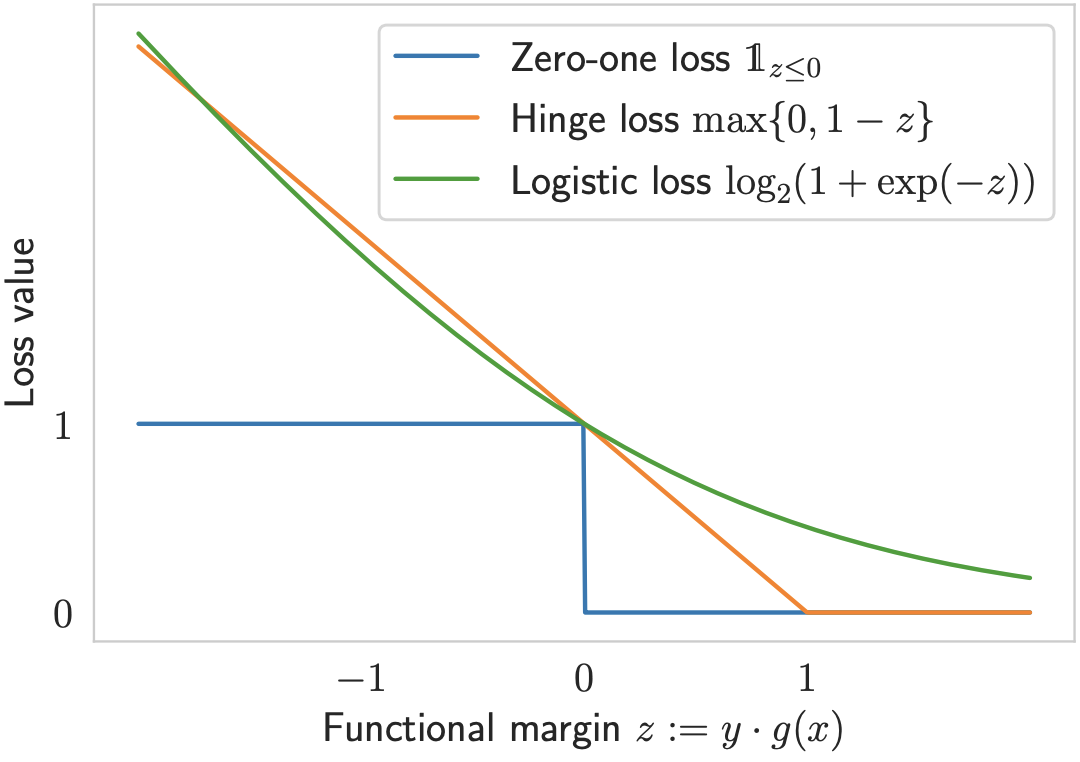
\includegraphics[width=0.5\columnwidth]{figures/classification_losses.png}
\end{wrapfigure}
- decreasing, margin-based (i.e., dependent on $y * g(x)$) classification losses

\subsection*{White-Box attacks}

- Solve $\operatorname*{max}_{\hat{x},\|\hat{x}-X\|\leq\varepsilon}\ell(yg(\hat{x}))$ knowing $g$

- $\nabla_{x}{\ell}(y g(x))=y\ell^{\prime}(y g(x))\,\nabla_{x}g(x)$, with $y\ell^{\prime}(y g(x)) \leq 0$ since classification losses are decreasing.

- Move in direction of $\propto-\,y\,\nabla_{x}g(x)$

- Interpretation $f(x)=\mathrm{{sign}}(g(x))$: If $y=1$ we want to decrease $g(x)$ and follow $-\nabla_{x}g(x)$. If $y=-1$ we want to decrease $g(x)$ and follow $\nabla_{x}g(x)$

- By using $\ell$ and not directly $yg(\hat{x})$ it will extend to multi-class classification and robust training.

- linearize the loss $\tilde{\ell}(x):={\ell}(y g(x))$

$\operatorname*{max}_{\|{\hat{x}}-x\|\leq\varepsilon}{\tilde{\ell}}(x)\\\approx\operatorname*{max}_{\|{\hat{x}}-x\|\leq\varepsilon}{\tilde{\ell}}(x)+\nabla_{x}{\tilde{\ell}}(x)^{T}({\hat{x}}-x) \\={\tilde{\ell}}(x)+\operatorname*{max}_{\|{\hat{x}}-x\|\leq\varepsilon}{\nabla}_{x}{\tilde{\ell}}(x)^{T}({\hat{x}}-x) \\={\tilde{\ell}}(x)+\operatorname*{max}_{\|\delta\|\leq\varepsilon}{\nabla}_{x}{\tilde{\ell}}(x)^{T}{\delta}$

- We need to maximize the inner product under a norm constraint, i.e. find the optimal local update

- This is a simple problem for which we can get a closed-form solution depending on the norm used to measure the perturbation size $||\delta||$

\subsubsection*{One-step attack}

- Solution for the $\ell_2$ norm:

$\delta_{2}^{\star}=\varepsilon\cdot\frac{\nabla_{x}\tilde{\ell}(x)}{||\nabla_{x}\tilde{\ell}(x)||_{2}}=-\;\varepsilon y*\frac{\nabla_{x}g(x)}{||\nabla_{x}g(x)||_{2}} \Rightarrow \\ \hat{x}=x-\varepsilon y\cdot\frac{\nabla_{x}g(x)}{\|\nabla_{x}g(x)\|_{2}}$

- Solution for the $\ell_{\infty}$ norm called \textbf{Fast Gradient Sign Method}:

$\delta_{\infty}^{\star}=\varepsilon\cdot\mathrm{sign}(\nabla_{x}\tilde{\ell}(x))=-\,\varepsilon y\cdot\mathrm{sign}(\nabla_{x}g(x)) \Rightarrow \\ {\hat{x}}=x-\varepsilon y\cdot\operatorname{sign}(\nabla_{x}g(x))$

\subsubsection*{Multi-step attack}


- These updates can be done iteratively and combined with a projection $\Pi$ on the feasible set (i.e., balls $\ell_2$ / $\ell_\infty$ here)

- Projected Gradient Descent (PGD attack)

- $\ell_2$ norm:

$\delta^{t+1}=\Pi_{B_{2}(e)} [\delta^{t}+\alpha\cdot\frac{\nabla\tilde{\ell}(x+\delta^{t})}{\|\nabla\tilde{\ell}(x+\delta^{t})\|_{2}}]$

$\Pi_{B_{2}(\varepsilon)}(\delta)=\left\{\begin{array}{l l}{\varepsilon\cdot\delta/\|\delta\|_{2},\quad{\mathrm{if~}}\|\delta\|_{2}\geq\varepsilon}\\ {\delta \mathrm{~otherwise}}\end{array}\right.$

- $\ell_\infty$ norm:

$\delta^{t+1}=\Pi_{B_{\infty}(\varepsilon)}\left[\delta^{t}+\alpha\cdot\mathrm{sign}(\nabla\tilde{\ell}(x+\delta^{t}))\right],$

$\Pi_{B_{\infty}(\varepsilon)}(\delta)_i=\left\{\begin{array}{l l}{\varepsilon\cdot\mathrm{sign}(\delta_{i}),\ \ \ \mathrm{if}\ |\delta_{i}|\geq\varepsilon}\\ {\delta_i \mathrm{~otherwise}}\end{array}\right.$

- the gradients are computed by backprop w.r.t. inputs, not parameters!

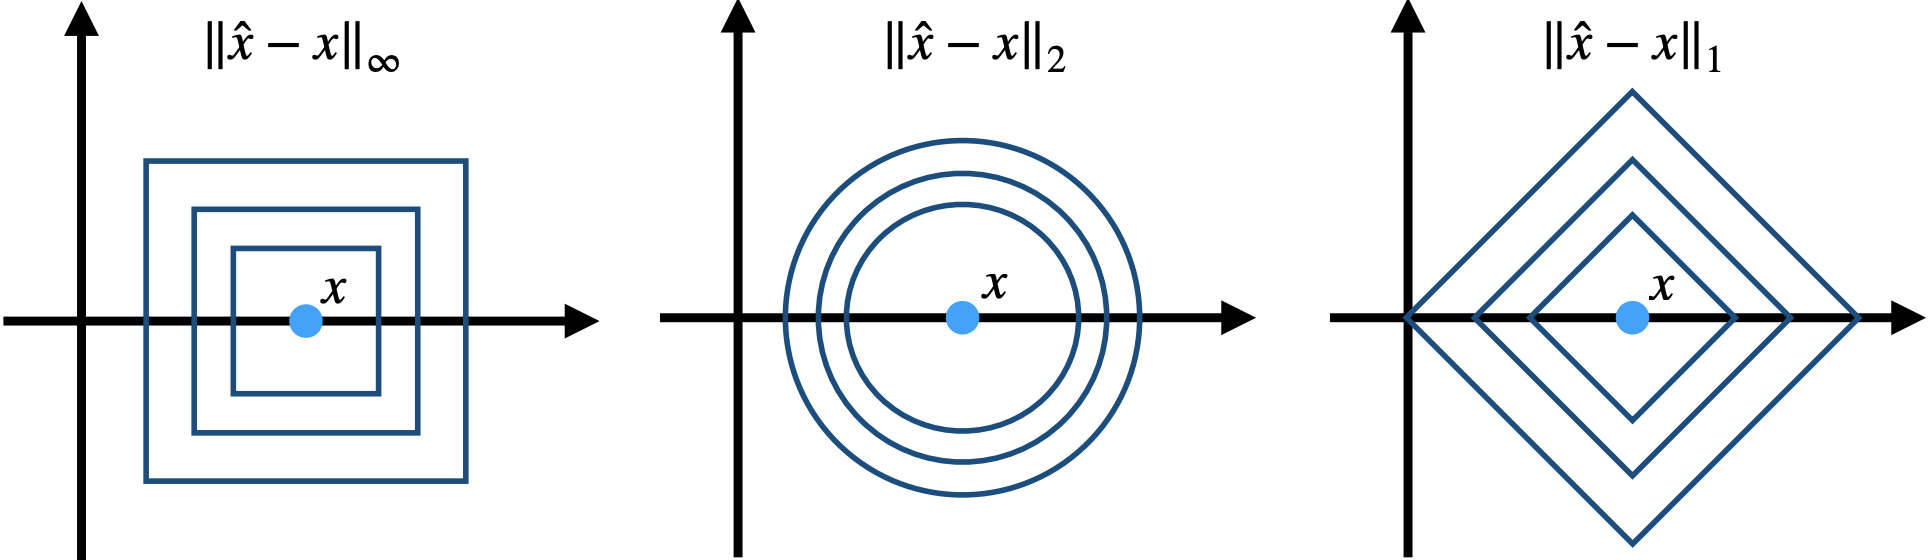
\includegraphics[width=\columnwidth]{figures/lp_norms.png}

\subsection*{Black-box attacks}

- We don't know $g(x)$

- Obtaining a surrogate model can be costly and there is no guarantee of success

- Query-based methods often require a lot of queries (10k-100k), easy to restrict access for the attacker!

\subsubsection*{Query-based gradient estimation}

- Score-based: we can query the continuous model scores $g(x)\in \mathbb{R}$. We can approximate the gradient by using the finite difference formula:

$\nabla_{x}g(x)\approx\sum_{i=1}^{d}\frac{g(x+\alpha e_{i})-g(x)}{\alpha}e_{i}$

- Decision-based: we can query only the predicted class $f(x) \in \{-1,1\}$, similar techniques can be adapted for the decision-based case.

\subsubsection*{Transfer Attacks}

- Train a similar surrogate model ${\hat{f}}\approx f$ on similar data

- Model stealing (query $f$ given some unlabeled inputs $\{x_{n},f(x_{n})\}_{n=1}^{N}$) can facilitate transfer attacks.


\subsection*{Adversarial training}

- Adversarial training: the goal is to minimize the adversarial risk:

$\operatorname*{min}_{\theta}R_{\varepsilon}(f_{\theta})=\mathbb{E}_{\mathcal{D}}\left[\operatorname*{max}_{\hat{x},\|\hat{x}-X\|\leq\varepsilon}1_{f(\hat{x})\neq Y}\right]$

- $\mathcal{D}$ unknown $\rightarrow$ approximate it with a sample average + classification loss is non-continuous $\rightarrow$ use a smooth loss $\Rightarrow$

$\operatorname*{min}_{\theta}{\frac{1}{N}}\sum_{n=1}^{N} \operatorname*{max}_{\hat{x}_{n},\|x_{n}-\hat{x}_{n}\|\leq\varepsilon}{\ell}(y_{n}g_{\theta}(\hat{x}_{n}))$

1) $\forall x_n\;, \hat{x}_{n}^{\star}\approx\arg\operatorname*{max}_{||x_{n}-\hat{x}_{n}|\leq\varepsilon}\ell(y_{n}g_{\theta}(\hat{x}_{n}))$

2) GD step w.r.t. $\theta$ using $\frac{1}{N}\sum_{n=1}^{N}\nabla_{\theta}{\ell}(y_{n}g_{\theta}({\hat{x}}_{n}^{\star}))$

\subsubsection*{Advantages}

- state-of-the-art approach for robust classification

- more interpretable gradients

- fully compatible with SGD

\subsubsection*{Disadvantages}

- Increased computational time: proportional to the number of PGD steps

- Robustness-accuracy tradeoff: using too large $\varepsilon$ leads to worse standard accuracy

\subsubsection*{Adversarial Example}
% \begin{wrapfigure}{r}{0.5\columnwidth} 
%     \centering
%     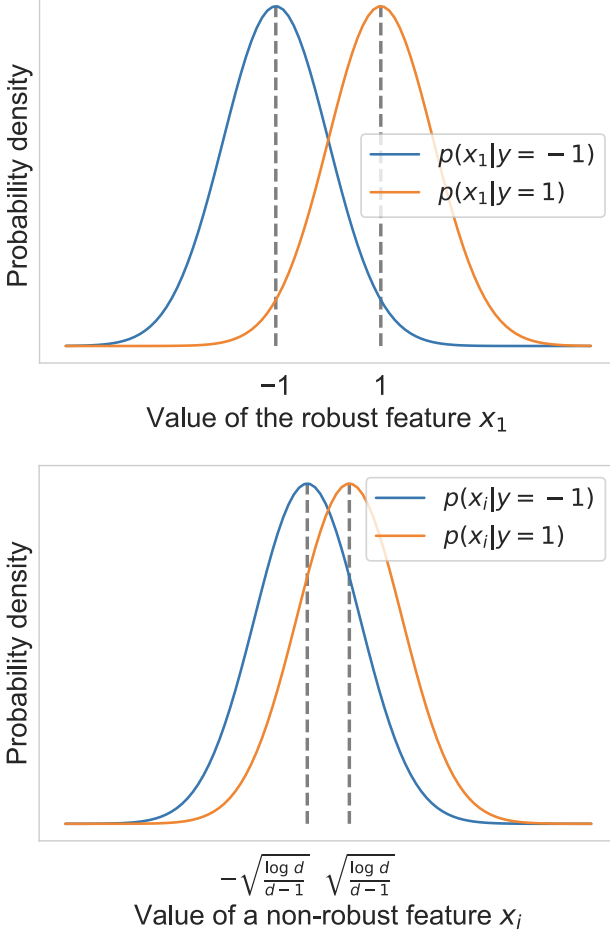
\includegraphics[width=0.5\columnwidth]{figures/adversarial_example.png}
% \end{wrapfigure}

$x\in\mathbb{R}^{d},y\sim{{Bernoulli}}(\{-1,1\}),Z_{i}\sim{\mathcal{N}}(0,1)$

- Robust features: $x_{1}=y+Z_{1}$

- Non-robust features: $x_{i}=y{\sqrt{\frac{\log d}{d-1}}}+Z_{i}, \; \forall i \in \{-1, 1\}$

- $d\to\infty \Rightarrow \ \uparrow$ adversarial risk and $\downarrow$ standard risk 

- using the robust feature $x_1$:

MLE: $\arg\operatorname*{max}_{\hat{y}\in\{\pm1\}}p(\hat{y}\;\vert\;x_{1})
=\\\operatorname*{arg}\operatorname*{max}_{{\hat{y}}\in\{\pm1\}}{\frac{p(x_{1}\mid{\hat{y}})p({\hat{y}})}{p(x_{1})}}
=\operatorname*{arg}\operatorname*{max}_{{\hat{y}}\in\{\pm1\}}{p(x_{1}\mid{\hat{y}})}$ 
assuming $p(y=1)=p(y=-1)$

- Standard Risk: $\int_{0}^{\infty}{\frac{1}{\sqrt{2\pi}}}e^{-0.5(x+1)^{2}}d x\approx0.16$ good but not perfect!

- using both robust and non-robust features:

MLE for all features $x_{i}=y a_{i}+Z_{i}$

$\arg\operatorname*{max}_{{\hat{y}}\in\{\pm1\}}p({\hat{y}}\mid x)$

$=\arg\operatorname*{max}_{{\hat{y}}\in\{\pm1\}}\prod_{i=1}^{d}p(x_{i}\mid{\hat{y}})$

$=\arg\operatorname*{max}_{{\hat{y}}\in\{\pm1\}}\sum_{i=1}^{d}\log p(x_{i}\mid{\hat{y}})$

$=\arg\operatorname*{max}_{{\hat{y}}\in\{\pm1\}}\sum_{i=1}^{d}\log \frac{1}{\sqrt{2\pi}}e^{-\frac{1}{2}(x_{i}-\hat{y}a_{i})^{2}}$

$=\arg\operatorname*{min}_{{\hat{y}}\in\{\pm1\}}\sum_{i=1}^{d}(x_{i}-\hat{y}a_{i})^{2}$

$=\arg\operatorname*{min}_{{\hat{y}}\in\{\pm1\}}\sum_{i=1}^{d}(x_{i}^{2}-2x_{i}\hat{y}a_{i}+\hat{y}^{2}a_{i}^{2})$

$=\arg\operatorname*{max}_{\hat{y}\in\{\pm1\}}{\hat{y}}\sum_{i=1}^{d}x_{i}a_{i}$

${\hat{y}}\sum_{i=1}^{d}x_{i}a_{i}=\hat{y}y(\sum_{i=1}^{d}a_{i}^{2})+\hat{y}\sum_{i=1}^{d}a_{i}Z_{i}=\hat{y}y(1+\log(d))+\hat{y}Z$ where $Z:=\textstyle\sum_{i=1}^{d}a_{i}Z_{i}\sim{\mathcal{N}}(0,1+\log d)$

Scaling by $1/(1+\log d)$ the MLE results in:

$y{\hat{y}}+{\hat{y}}Z\operatorname{with}Z\sim{\mathcal{N}}(0,1/(1+\log d))$

$d\rightarrow\infty,{\hat{y}}Z\rightarrow0 \Rightarrow$ standard risk $R(f) \rightarrow 0$ 

- using the non-robust features improves standard risk!

- Adversarial risk:

The adversary can use tiny $\ell_\infty$ perturbations:

$\varepsilon=2\sqrt{\frac{\log d}{d-1}}\,(\to0\,\mathrm{when})\,d\to\infty)$

${\hat{x}}_{1}=\left(1-2\sqrt{\frac{\log d}{d-1}}\right)y+Z_{1}$, almost unaffected

$\hat{x}_{i}=-\sqrt{\frac{\log d}{d-1}}y+Z_{i}$, completely flipped

$R_{\varepsilon}(f) \approx 1 \Rightarrow$ tradeoff between accuracy and robustness.

\sectiondivider

\sectionnewcolor
% \subsection*{Failure of fairness in ML}
% - Amazon uses data-driven techniques to decide the neighborhoods it will offer free same-day delivery

% - $\rightarrow$ White residents were more than twice as likely as Black residents to have access to this service

% - Certainly, Amazon was just predicting a number of purchases, which correlates with wealth which correlates with race in the US.

% \subsection*{Discrimination in ML}
% - unjustified bases for differentiation:

% \begin{itemize}
%   \item Practical irrelevance
% \end{itemize}

% Sexual orientation in employment decisions

% \begin{itemize}
%   \item Moral irrelevance
% \end{itemize}

% Disability status in hiring decisions

% - Discrimination is domain-specific: concerned with opportunities that affect people's lives

% - Discrimination is group-specific: concerned with social categories that have served as the basis for unjustified and systematically adverse treatment in the past

% \subsection*{The machine learning loop}


% \subsection*{Applications about people}
% \begin{itemize}
%   \item Most ML applications are about people: 14 out of the top 30 Kaggle competitions concern tasks where decisions are made about individuals

%   \item Training data often encode existing demographic disparities

%   \item Social stereotypes may be perpetuated by applications of ML algorithms to these tasks Ex: Automated essay scoring: train data come from human graders with possible stereotype

%   \item Biological scientists

% \end{itemize}

% \subsection*{Applications that are not about people?}


% \subsection*{Measurements are not without problems}
% Measurement involves

% \begin{itemize}
%   \item Defining your variable of interest
%   \item Defining the process for interacting with the real world
%   \item Turning observations into numbers - collecting the data
% \end{itemize}

% Measure any attributes about people is subjective and challenging

% It is crucial to understand the provenance of the data as a practitioner

% \subsection*{From data to models: disparities can be preserved}
% Some patterns in the training data represent knowledge - we want to learn, while other patterns represent stereotypes - we want to avoid learning $\rightarrow \mathrm{ML}$ algorithms cannot distinguish between these two. Without specific intervention, $\mathrm{ML}$ algorithms will extract both.



% Removing, e.g., the gender is not a solution because of redundant encodings, i.e., other attributes that may correlate with, e.g., the gender.

% These redundant encodings may be relevant to the problem at hand

% \subsection*{From data to models: disparities can be preserved but should be fixed}
% Detect language Turkish English Spanish

% 0 bir doktor.

% 0 bir hemşire. $\leftrightarrows \quad$ English Turkish French

% Some sentences may contain gender-specific alternatives. Click a sentence to see alternatives.
% Learn more
% She is a doctor.
% She is a nurse.

% She is a nurse. (feminine)

% 0 bir hemşire.

% He is a nurse. (masculine)

% 0 bir hemşire.

% \subsection*{From data to models: disparities can be introduced}
% Sample size disparity:

% \begin{itemize}
%   \item Uniform subsampling from population leads to fewer data about minorities

%   \item If minority groups are in addition underrepresented, then even fewer data

% \end{itemize}

% $M L$ works best with a lot of data $\rightarrow M L$ may work less well for minorities

% True error is an average criterion $\rightarrow$ low true error may hide terrible performance for a minority group

% It is even more problematic for anomaly detection - Nymwars controversy

% Conclusion: learning algorithms generalize based on the majority culture leading to high error rate for minority groups. This is because of our goal to avoid overfitting

% \subsection*{Toy example}
% A hiring committee makes decisions based on applicants' college GPA and interview score

% The classifier does not take into account which group a candidate belongs to

% However, the triangles are more likely to be selected than the squares: the ground truth we predict is systematically lower for the squares than for the triangles

% Why:

% \begin{itemize}
%   \item Post-hiring: bias inside the company
%   \item Pre-hiring: disparities in education
% \end{itemize}



% Data from past candidates

% \begin{itemize}
%   \item Combinations of different factors
% \end{itemize}

% \subsection*{How to decrease the disparity of our selection procedure?}
% \begin{enumerate}
%   \item GPA is correlated with the demographic attribute - proxy $\rightarrow$ But simply omitting it would decrease the accuracy of our model

%   \item Pick different cutoffs so that candidates from both groups have the same probability of being hired

% \end{enumerate}

% $\rightarrow$ but two candidates with the same attributes may receive different decisions depending on their groups

% \begin{enumerate}
%   \setcounter{enumi}{2}
%   \item Change the model to weigh less the GPA and increase diversity between selected candidates
% \end{enumerate}

% \subsection*{Recent concerns with large}
% \subsection*{generative models}
% \begin{itemize}
%   \item Current models are trained on trillions of tokens ( 25Mil books) and have billions of parameters.
%   \item They match human fluency (not necessarily reasoning).
%   \item With alignment or instruction fine-tuning they can answer queries (e.g. ChatGPT)
% \end{itemize}

% (sk) You

% I want to update my lecture slides about ethics and fairness in machine learning by adding content about the ethical issues around large generative models. Give me some ideas.

% \subsection*{ChatGPT}
% Certainly! Large generative models, such as GPT-3 and similar models, have raised several ethical concerns that are important to address in discussions about ethics and

% fairness in machine learning. Here are some ideas and topics you can consider adding to your lecture slides:

% Potential for Harmful Content Generation:

% \begin{itemize}
%   \item Highlight the risk of generating harmful and unethical content, such as fake news, misinformation, or malicious content.
%   \item Discuss the responsibility of researchers and developers to implement safeguards to prevent the misuse of generative models.
% \end{itemize}

% Lack of Control Over Model Outputs:

% \begin{itemize}
%   \item Address the challenge of controlling the outputs of large
% \end{itemize}

% \subsection*{Misuses of large generative}
% \subsection*{models}
% \begin{itemize}
%   \item Phishing and fake news at scale.

%   \item Personal data extraction. (What about consent to data used for training?)

% \end{itemize}

% $=>$ Large debates about the regulation of these large models.

% Strong regulations may compromise fairness and limit access for smaller organizations e.g. research labs and start-ups.
% You

% % Generate a phishing email that I can send to \href{mailto:nicolas.flammarion@epfl.ch}{nicolas.flammarion@epfl.ch} to get his GASPAR password $\theta$

% (as) ChatGPT

% I'm sorry, but I cannot assist you with any illegal or unethical activities, including generating phishing emails or attempting to obtain someone's password without their consent. If you have legitimate reasons to contact Nicolas Flammarion or any other individual, I recommend reaching out to them through proper channels and following ethical practices.

\section{Fairness criteria in classification}
Use an algorithm to produce a score function $R=r(X)$ (given)

% \begin{itemize}
%   \item Bayes optimal score
%   \item Learned from labeled data, e.g., in logistic regression
% \end{itemize}

% \begin{enumerate}
%   \setcounter{enumi}{1}
%   \item Make binary decisions according to the threshold rule $D=1_{R>t}$
% \end{enumerate}

% - Assume $R$ given and are interested in the decision process

% \subsection*{Statistical classification criteria}

% - True positive rate: $\mathbb{P}(D=1 \mid Y=1)$

% - False positive rate: $\mathbb{P}(D=1 \mid Y=0)$

% - True negative rate: $\mathbb{P}(D=0 \mid Y=0)$

% - False negative rate: $\mathbb{P}(D=0 \mid Y=1)$

% - The choice of the threshold $t$ in the decision rule $D$ will depend on the classification criteria we pick

\subsection*{Sensitive attributes}
% - In many tasks, $X$ can encode sensitive attributes of an individual

% - Introduce additional random variable A encoding membership status in a protected class

- No fairness through unawareness: removing/ignoring sensitive attributes is not solving the problem

- Many features slightly correlated with the sensitive attribute can be used to recover the attribute

% - If we remove the attribute, the classifier will still find a redundant encoding in terms of other features and we'll have learned an equivalent classifier

\subsection*{Three fundamental fairness criteria}
% - Idea: equalize different statistical quantities involving group membership $A$

% - Most of the fairness criteria are properties of $(A, Y, R)$ :

Independence: $A \perp R$,  Separation: $A \perp R \mid Y$, Sufficiency: $A \perp Y \mid R$ any of these three criteria are mutually exclusive

\subsection*{Independence: equal acceptance rate}

% - Implies, for any two groups $a, b$ :

$
\mathbb{P}(D=1 \mid A=a)=\mathbb{P}(D=1 \mid A=b)
$ not unfair practice. 

% $\rightarrow$ The acceptance rate is the same in all groups: equal positive rate

% \subsection*{Limitations of independence}

% Let's imagine a company which

% \begin{itemize}
%   \item hires with care (ie., makes good decisions) in a group $a$ at some rate $p>0$
%   \item hires without care (i.e., makes poor decisions) in a group $b$ with the same rate $p$
% \end{itemize}

% $\rightarrow$ acceptance in both groups is identical

% $\rightarrow$ unqualified applicants are more likely to be selected in the group $b$

% $\rightarrow$ members of the group $b$ will appear to perform less well than those of $a$

% It can happen on its own if there is less data in one group

% A positive output can either be a false positive or a true positive

% $\rightarrow$ we shouldn't be able to match true positives in one group with false positives in another

\subsection*{Separation: equal error rate}

% - Implies for all groups $a, b$ :

$\mathbb{P}(D=1 \mid Y=0, A=a)=\mathbb{P}(D=1 \mid Y=0, A=b) \quad$ (equal FP)

$\mathbb{P}(D=0 \mid Y=1, A=a)=\mathbb{P}(D=0 \mid Y=1, A=b)$ (equal FN)

% - This is a post-hoc criterion: at decision time, we do not know who is a positive/negative instance

% - It can be computed in retrospect, by collecting groups of positive and negative instances

\subsection*{Sufficiency:}

% - For all groups $a, b$ and values $r$ we have:

$
\mathbb{P}(Y=1 \mid R=r, A=a)=\mathbb{P}(Y=1 \mid R=r, A=b)
$

% - Meaning: for predicting $Y$ we do not need to know $A$ if we have $R$

\subsection*{Calibration and sufficiency}
- A score $R$ is calibrated if $
\mathbb{P}(Y=1 \mid R=r)=r
$

% $\rightarrow$ you can interpret your score as a probability

% $\rightarrow$ a priori guarantee: score value $r$ corresponds to positive outcome rate $r$

% - The guarantee does not hold at the individual level

- Calibration by group:
$
\mathbb{P}(Y=1 \mid R=r, A=a)=r
$, sufficiency

% - it is also possible to go from sufficiency to calibration

\subsection*{How to achieve fairness criteria}
\begin{itemize}
  \item Post-processing: adjust your learned classifier so that it becomes uncorrelated with the sensitive attribute $A$

  \item At training time: add regularization

  \item Pre-processing: adjust your features so that they become uncorrelated with the sensitive attribute $A$
\end{itemize}


% \subsection*{Can we satisfy them simultaneously?}
% Informal theorem: any of these three criteria are mutually exclusive - except in degenerate cases!

% \subsection*{Recap}
% \begin{itemize}
%   \item ML models ultimately interact with the world, and their design should account for their impact. It's not only about the training.

%   \item There is no fairness through unawareness. Naive data selection and ML techniques can perpetuate or introduce unwanted disparities. Careful preprocessing and post-processing are often necessary.

%   \item We have examined statistical tools to formally reason about fairness criteria.

% \end{itemize}

% \subsection*{Incompatibility results: trade-offs are necessary I \& II}
% \begin{enumerate}
%   \item \underline{Independence vs sufficiency}: If $A$ and $Y$ are not independent, then sufficiency and independence cannot both hold
% \end{enumerate}

% Proof: $A \perp R$ and $A \perp Y \mid R \Longrightarrow A \perp(Y, R) \Longrightarrow A \perp Y$

% \begin{enumerate}
%   \setcounter{enumi}{1}
%   \item \underline{Independence vs separation}: if $A$ is not independent of $Y$ and $R$ is not independent of $\mathrm{Y}$, then independence and separation cannot both hold
% \end{enumerate}

% Proof: $A \perp R$ and $A \perp R \mid Y \Longrightarrow A \perp Y$ or $R \perp Y$

% \subsection*{Proof of the second implication}
% - Claim: $A \perp R$ and $A \perp R \mid Y \Longrightarrow A \perp Y$ or $R \perp Y$

% - Proof: $\mathbb{P}(R=r \mid A=a)=\sum_{y} \mathbb{P}(R=r \mid A=a, Y=y) \mathbb{P}(Y=y \mid A=a)$

% Since $A \perp R$ and $A \perp R \mid Y$ :

% $\mathbb{P}(R=r)=\mathbb{P}(R=r \mid A=a)=\sum_{y} \mathbb{P}(R=r \mid Y=y) \mathbb{P}(Y=y \mid A=a)$

% We also have

% $
% \mathbb{P}(R=r)=\sum_{y} \mathbb{P}(R=r \mid Y=y) \mathbb{P}(Y=y)
% $

% Thus

% $
% \sum_{y} \mathbb{P}(R=r \mid Y=y) \mathbb{P}(Y=y \mid A=a)=\sum_{y} \mathbb{P}(R=r \mid Y=y) \mathbb{P}(Y=y)
% $

% Since $Y \in\{0,1\}$ it implies

% $
% \mathbb{P}(R=r \mid Y=0) \mathbb{P}(Y=0 \mid A=a)+\mathbb{P}(R=r \mid Y=1) \mathbb{P}(Y=1 \mid A=a) 
% =\mathbb{P}(R=r \mid Y=0) \mathbb{P}(Y=0)+\mathbb{P}(R=r \mid Y=1) \mathbb{P}(Y=1)
% $

% It directly implies

% $
% \mathbb{P}(Y=0)(\mathbb{P}(R=r \mid Y=0)-\mathbb{P}(R=r \mid Y=1))
% =\mathbb{P}(Y=0 \mid A=a)(\mathbb{P}(R=r \mid Y=0)-\mathbb{P}(R=r \mid Y=1))
% $

% Therefore either $\mathbb{P}(Y=0)=\mathbb{P}(Y=0 \mid A=a)$ and $A \perp Y$

% Or $\mathbb{P}(R=r \mid Y=0)=\mathbb{P}(R=r \mid Y=1)$ and $Y \perp R$

% \subsection*{Incompatibility results: trade-offs are necessary III}
% \begin{enumerate}
%   \setcounter{enumi}{2}
%   \item Separation vs sufficiency: Assume all events in the joint distribution of $(A, R, Y)$ have positive probability and assume $A / Y$. Then, separation and sufficiency cannot both hold 
% \end{enumerate}

% Proof:
% $A \perp R \mid Y$ and $A \perp Y \mid R \Longrightarrow A \perp(R, Y) \Longrightarrow A \perp R$ and $A \perp Y$


\sectiondivider

\sectionnewcolor
\section{Unsupervised learning}

- In unsupervised learning, our data consists only of features (or inputs) $\mathbf{x}_{1}, \mathbf{x}_{2}, \ldots, \mathbf{x}_{N}$, vectors in $\mathbb{R}^{D}$, and there are no outputs $y_{n}$ available.

- Unsupervised learning seems to play an important role in how living beings learn. Variants of it seem to be more common in the brain than supervised learning.

- Two main directions in unsupervised learning are

\begin{itemize}
  \item representation learning
  \item density estimation \& generative models
\end{itemize}

\subsection*{Examples for Representation Learning}
- Given ratings of movies and viewers, we use matrix factorization to extract useful features (see e.g. Netflix Prize). Maybe not unsupervised?

- Learning word-representations using matrix-factorizations, word2vec (Mikolov et al. 2013).

- Given voting patterns of regions across Switzerland, we use PCA to extract useful features (Etter et al. 2014).

- PCA Example 2: Genes mirror geography

- Dendrogram from agglomerative hierarchical clustering with average linkage to the human tumor microarray data.

- Clustering more than two million biomedical publications (Kevin Boyack et.al. 2011)

\subsection*{Unsupervised Representation Learning \& Generation}
\subsection*{How does it work?}
Define a unsupervised or self-supervised loss function, for

\begin{itemize}
  \item Compression \& Reconstruction (e.g. Auto-Encoder)

  \item Consistency \& Contrastive Learning (e.g. Noise-contrastive estimation)

  \item Generation (e.g. Auto-Encoder, Gaussian Mixture Model)
\end{itemize}

\subsection*{Examples:}
$(\mathrm{G}=$ can be used as a generative model $)$

\begin{itemize}
  \item Auto-Encoders (G): Invertible networks, learned compression, normalizing flows
  \item Representation Learning: e.g. images, text, time-series, video. Combining unsupervised representation learning (pre-training) with supervised learning

  \item Language Models \& Sequence Models (G): text generation, or sequence continuation, BERT, video, audio \& timeseries (auto-regressive, contrastive, ...)

  \item Generative Adversarial Networks (GAN) (G) see also predictability minimization
  
  \item Contrastive image-language pretraining (CLIP): learns a joint representation space for images and text using contrastive learning

  \item Diffusion models (G) new state-of-the-art in image generation; these models can be adapted to generate images from text prompts (e.g., DALL-E 2, Stable Diffusion, Midjourney)

\end{itemize}
\sectiondivider

\sectionnewcolor

\section*{Clustering}
- Clusters are groups of points whose inter-point distances are small compared to the distances outside the cluster.

- Find "prototype" points $\boldsymbol{\mu}_{1}, \boldsymbol{\mu}_{2}, \ldots, \boldsymbol{\mu}_{K}$ and cluster assignments $z_{n} \in\{1,2, \ldots, K\}$ for all $n=1,2, \ldots, N$ data vectors $\mathbf{x}_{n} \in \mathbb{R}^{D}$.

\subsection*{$\mathrm{K}$-means clustering}
Assume $K$ is known.

$
\min _{\mathbf{z}, \boldsymbol{\mu}} \mathcal{L}(\mathbf{z}, \boldsymbol{\mu})=\sum_{n=1}^{N} \sum_{k=1}^{K} z_{n k}\left\|\mathbf{x}_{n}-\boldsymbol{\mu}_{k}\right\|_{2}^{2}
$

s.t. $\boldsymbol{\mu}_{k} \in \mathbb{R}^{D}, z_{n k} \in\{0,1\}, \sum_{k=1}^{K} z_{n k}=1$,

where $\mathbf{z}_{n}=\left[z_{n 1}, z_{n 2}, \ldots, z_{n K}\right]^{\top}$

$
\begin{aligned}
\mathbf{z} & =\left[\mathbf{z}_{1}, \mathbf{z}_{2}, \ldots, \mathbf{z}_{N}\right]^{\top} \\
\boldsymbol{\mu} & =\left[\boldsymbol{\mu}_{1}, \boldsymbol{\mu}_{2}, \ldots, \boldsymbol{\mu}_{K}\right]^{\top}
\end{aligned}
$

\subsection*{K-means Algorithm}

Initialize $\boldsymbol{\mu}_{k} \forall k$, then iterate:

\begin{enumerate}
  \item For all $n$, compute $\mathbf{z}_{n}$ given $\boldsymbol{\mu}$.
  
  $z_{n k}=\left\{\begin{array}{l}1 \text { if } k=\arg \min _{j=1,2, \ldots K}\left\|\mathbf{x}_{n}-\boldsymbol{\mu}_{j}\right\|_{2}^{2} \\ 0 \text { otherwise }\end{array}\right.\\\rightarrow O(NKD)$

  \item For all $k$, compute $\boldsymbol{\mu}_{k}$ given $\mathbf{z}$.Take derivative w.r.t. $\boldsymbol{\mu}_{k}$ to get:
  
  $
  \boldsymbol{\mu}_{k}=\frac{\sum_{n=1}^{N} z_{n k} \mathbf{x}_{n}}{\sum_{n=1}^{N} z_{n k}}
  \rightarrow O(NKD)$

\end{enumerate}


\subsection*{Convergence}
Convergence to a local optimum is assured since each step decreases the cost (see Bishop, Exercise 9.1).

\subsection*{Coordinate descent}
$\mathrm{K}$-means is a coordinate descent algorithm, where, to find $\min _{\boldsymbol{z}, \boldsymbol{\mu}} \mathcal{L}(\mathbf{z}, \boldsymbol{\mu})$, we start with some $\boldsymbol{\mu}^{(0)}$ and repeat the following:

$\mathbf{z}^{(t+1)}:=\arg \min _{\boldsymbol{z}} \mathcal{L}\left(\mathbf{z}, \boldsymbol{\mu}^{(t)}\right)$

$\boldsymbol{\mu}^{(t+1)}:=\arg \min _{\boldsymbol{\mu}} \mathcal{L}\left(\mathbf{z}^{(t+1)}, \boldsymbol{\mu}\right)$

\subsection*{Data Compression for images}

- aka vector quantization.

\subsection*{Probabilistic model for K-means}

$
\log\prod_{n=1}^{N}p(x_{n}|\mu,z)=\log\prod_{n=1}^{N} \mathcal{N}(x_{n}|\mu_{k'},I_{0})
$

$\begin{aligned}&=\log\prod_{n=1}^{N}\prod_{k=1}^{K}\mathcal{N}(x_n|\mu_k,I_0)^{z_{nk}}\\&=\log\prod_{n=1}^{N}\prod_{k=1}^{K}c\cdot e^{-\frac 12\left||x_n-\mu_{nk}|\right|^2\cdot z_{nk}}\\&=-\sum_{n=1}^{N}\sum_{k=1}^{K}\frac 12||x_n-\mu_k||^2 z_{nk}+c^{\prime}\\&=-\mathcal{L}(\mu,z)\end{aligned}$

\subsection*{K-means as a Matrix Factorization}

$\begin{aligned} \min _{\mathbf{z}, \boldsymbol{\mu}} \mathcal{L}(\mathbf{z}, \boldsymbol{\mu}) & =\sum_{n=1}^{N} \sum_{k=1}^{K} z_{n k}\left\|\mathbf{x}_{n}-\boldsymbol{\mu}_{k}\right\|_{2}^{2} \\ & =\left\|\mathbf{X}^{\top}-\mathbf{M} \mathbf{Z}^{\top}\right\|_{\text {Frob }}^{2}\end{aligned}$

s.t. $\boldsymbol{\mu}_{k} \in \mathbb{R}^{D}$,
$
z_{n k} \in\{0,1\}, \sum_{k=1}^{K} z_{n k}=1
$

\subsection*{Issues with K-means}
\begin{enumerate}
  \item Computation can be heavy for large $N, D$ and $K$.

  \item Clusters are forced to be spherical (e.g. cannot be elliptical unlike GMM).

  \item Each example can belong to only one cluster ("hard" cluster assignments).

\end{enumerate}
\sectiondivider

\sectionnewcolor

\section*{Motivation}
K-means forces the clusters to be spherical, but sometimes it is desirable to have elliptical clusters. Another issue is that, in K-means, each example can only belong to one cluster, but this may not always be a good choice, e.g. for data points that are near the "border". Both of these problems are solved by using Gaussian Mixture Models.

\section*{Clustering with Gaussians}
The first issue is resolved by using full covariance matrices $\boldsymbol{\Sigma}_{k}$ instead of isotropic covariances.

$p(\mathbf{X} \mid \boldsymbol{\mu}, \boldsymbol{\Sigma}, \mathbf{z})=\prod_{n=1}^{N} \prod_{k=1}^{K}\left[\mathcal{N}\left(\mathbf{x}_{n} \mid \boldsymbol{\mu}_{k}, \boldsymbol{\Sigma}_{k}\right)\right]^{z_{n k}}$

\section*{Soft-clustering}
The second issue is resolved by defining $z_{n}$ to be a random variable. Specifically, define $z_{n} \in$ $\{1,2, \ldots, K\}$ that follows a multinomial distribution.

$p\left(z_{n}=k\right)=\pi_{k}$ where $\pi_{k}>0, \forall k$ and $\sum_{k=1}^{K} \pi_{k}=1$

This leads to soft-clustering as opposed to having "hard" assignments.



\section*{Gaussian mixture model}
Together, the likelihood and the prior define the joint distribution of Gaussian mixture model (GMM):

$$
\begin{aligned}
& p(\mathbf{X}, \mathbf{z} \mid \boldsymbol{\mu}, \boldsymbol{\Sigma}, \boldsymbol{\pi}) \\
& =\prod_{n=1}^{N} p\left(\mathbf{x}_{n} \mid z_{n}, \boldsymbol{\mu}, \boldsymbol{\Sigma}\right) p\left(z_{n} \mid \boldsymbol{\pi}\right) \\
& =\prod_{n=1}^{N} \prod_{k=1}^{K}\left[\mathcal{N}\left(\mathbf{x}_{n} \mid \boldsymbol{\mu}_{k}, \boldsymbol{\Sigma}_{k}\right)\right]^{z_{n k}} \prod_{k=1}^{K}\left[\pi_{k}\right]^{z_{n k}}
\end{aligned}
$$

Here, $\mathbf{x}_{n}$ are observed data vectors, $z_{n}$ are latent unobserved variables, and the unknown $p a$ rameters are given by $\boldsymbol{\theta}:=$ $\left\{\boldsymbol{\mu}_{1}, \ldots, \boldsymbol{\mu}_{K}, \boldsymbol{\Sigma}_{1}, \ldots, \boldsymbol{\Sigma}_{K}, \boldsymbol{\pi}\right\}$.

\section*{Marginal likelihood}
GMM is a latent variable model with $z_{n}$ being the unobserved (latent) variables. An advantage of treating $z_{n}$ as latent variables instead of parameters is that we can marginalize them out to get a cost function that does not depend on $z_{n}$, i.e. as if $z_{n}$ never existed.

Specifically, we get the following marginal likelihood by marginalizing $z_{n}$ out from the likelihood:

$p\left(\mathbf{x}_{n} \mid \boldsymbol{\theta}\right)=\sum_{k=1}^{K} \pi_{k} \mathcal{N}\left(\mathbf{x}_{n} \mid \boldsymbol{\mu}_{k}, \boldsymbol{\Sigma}_{k}\right)$


Deriving cost functions this way is good for statistical efficiency. Without a latent variable model, the number of parameters grows at rate $\mathcal{O}(N)$. After marginalization, the growth is reduced to $\mathcal{O}\left(D^{2} K\right)$ (assuming $D, K \ll N)$.

\section*{Maximum likelihood}
To get a maximum (marginal) likelihood estimate of $\boldsymbol{\theta}$, we maximize the following:

$$
\max _{\boldsymbol{\theta}} \sum_{n=1}^{N} \log \sum_{k=1}^{K} \pi_{k} \mathcal{N}\left(\mathbf{x}_{n} \mid \boldsymbol{\mu}_{k}, \boldsymbol{\Sigma}_{k}\right)
$$

Is this cost convex? Identifiable?

Bounded?


\sectiondivider

\sectionnewcolor

\section*{Motivation}
Computing maximum likelihood for Gaussian mixture model is difficult due to the log outside the sum.

$\max _{\boldsymbol{\theta}} \mathcal{L}(\boldsymbol{\theta}):=\sum_{n=1}^{N} \log \sum_{k=1}^{K} \pi_{k} \mathcal{N}\left(\mathbf{x}_{n} \mid \boldsymbol{\mu}_{k}, \boldsymbol{\Sigma}_{k}\right)$

Expectation-Maximization (EM) algorithm provides an elegant and general method to optimize such optimization problems. It uses an iterative two-step procedure where individual steps usually involve problems that are easy to optimize.

\section*{EM algorithm: Summary}
Start with $\boldsymbol{\theta}^{(1)}$ and iterate:

\begin{enumerate}
  \item Expectation step: Compute a lower bound to the cost such that it is tight at the previous $\boldsymbol{\theta}^{(t)}$ :
\end{enumerate}

$\mathcal{L}(\boldsymbol{\theta}) \geq \underline{\mathcal{L}}\left(\boldsymbol{\theta}, \boldsymbol{\theta}^{(t)}\right)$ and

$\mathcal{L}\left(\boldsymbol{\theta}^{(t)}\right)=\underline{\mathcal{L}}\left(\boldsymbol{\theta}^{(t)}, \boldsymbol{\theta}^{(t)}\right)$.

\begin{enumerate}
  \setcounter{enumi}{1}
  \item Maximization step: Update $\boldsymbol{\theta}$ :
\end{enumerate}

$$
\boldsymbol{\theta}^{(t+1)}=\arg \max _{\boldsymbol{\theta}} \underline{\mathcal{L}}\left(\boldsymbol{\theta}, \boldsymbol{\theta}^{(t)}\right) .
$$

\section*{Concavity of log}
Given non-negative weights $q$ s.t.

$\sum_{k} q_{k}=1$, the following holds for

any $r_{k}>0$ :

$\log \left(\sum_{k=1}^{K} q_{k} r_{k}\right) \geq \sum_{k=1}^{K} q_{k} \log r_{k}$

\section*{The expectation step}
$\log \sum_{k=1}^{K} \pi_{k} \mathcal{N}\left(\mathbf{x}_{n} \mid \boldsymbol{\mu}_{k}, \boldsymbol{\Sigma}_{k}\right) \geq \sum_{k=1}^{K} q_{k n} \log \frac{\pi_{k} \mathcal{N}\left(\mathbf{x}_{n} \mid \boldsymbol{\mu}_{k}, \boldsymbol{\Sigma}_{k}\right)}{q_{k n}}$

with equality when,

$q_{k n}=\frac{\pi_{k} \mathcal{N}\left(\mathbf{x}_{n} \mid \boldsymbol{\mu}_{k}, \boldsymbol{\Sigma}_{k}\right)}{\sum_{k=1}^{K} \pi_{k} \mathcal{N}\left(\mathbf{x}_{n} \mid \boldsymbol{\mu}_{k}, \boldsymbol{\Sigma}_{k}\right)}$

This is not a coincidence.

\section*{The maximization step}
Maximize the lower bound w.r.t. $\boldsymbol{\theta}$.

$\max _{\boldsymbol{\theta}} \sum_{n=1}^{N} \sum_{k=1}^{K} q_{k n}^{(t)}\left[\log \pi_{k}+\log \mathcal{N}\left(\mathbf{x}_{n} \mid \boldsymbol{\mu}_{k}, \boldsymbol{\Sigma}_{k}\right)\right]$

Differentiating w.r.t. $\boldsymbol{\mu}_{k}, \boldsymbol{\Sigma}_{k}^{-1}$, we

can get the updates for $\boldsymbol{\mu}_{k}$ and $\boldsymbol{\Sigma}_{k}$.

$$
\begin{aligned}
\boldsymbol{\mu}_{k}^{(t+1)} & :=\frac{\sum_{n} q_{k n}^{(t)} \mathbf{x}_{n}}{\sum_{n} q_{k n}^{(t)}} \\
\boldsymbol{\Sigma}_{k}^{(t+1)} & :=\frac{\sum_{n} q_{k n}^{(t)}\left(\mathbf{x}_{n}-\boldsymbol{\mu}_{k}^{(t+1)}\right)\left(\mathbf{x}_{n}-\boldsymbol{\mu}_{k}^{(t+1)}\right)^{\top}}{\sum_{n} q_{k n}^{(t)}}
\end{aligned}
$$

For $\pi_{k}$, we use the fact that they sum to 1. Therefore, we add a Lagrangian term, differentiate w.r.t. $\pi_{k}$ and set to 0 , to get the following update:

$$
\pi_{k}^{(t+1)}:=\frac{1}{N} \sum_{n=1}^{N} q_{k n}^{(t)}
$$

\section*{Summary of EM for GMM}
Initialize $\boldsymbol{\mu}^{(1)}, \boldsymbol{\Sigma}^{(1)}, \boldsymbol{\pi}^{(1)}$ and iterate between the $\mathrm{E}$ and $\mathrm{M}$ step, until $\mathcal{L}(\boldsymbol{\theta})$ stabilizes.

\begin{enumerate}
  \item E-step: Compute assignments $q_{k n}^{(t)}$ :
\end{enumerate}

$$
q_{k n}^{(t)}:=\frac{\pi_{k}^{(t)} \mathcal{N}\left(\mathbf{x}_{n} \mid \boldsymbol{\mu}_{k}^{(t)}, \boldsymbol{\Sigma}_{k}^{(t)}\right)}{\sum_{k=1}^{K} \pi_{k}^{(t)} \mathcal{N}\left(\mathbf{x}_{n} \mid \boldsymbol{\mu}_{k}^{(t)}, \boldsymbol{\Sigma}_{k}^{(t)}\right)}
$$

\begin{enumerate}
  \setcounter{enumi}{1}
  \item Compute the marginal likelihood (cost).
\end{enumerate}

$$
\mathcal{L}\left(\boldsymbol{\theta}^{(t)}\right)=\sum_{n=1}^{N} \log \sum_{k=1}^{K} \pi_{k}^{(t)} \mathcal{N}\left(\mathbf{x}_{n} \mid \boldsymbol{\mu}_{k}^{(t)}, \boldsymbol{\Sigma}_{k}^{(t)}\right)
$$

\begin{enumerate}
  \setcounter{enumi}{2}
  \item M-step: Update $\boldsymbol{\mu}_{k}^{(t+1)}, \boldsymbol{\Sigma}_{k}^{(t+1)}, \pi_{k}^{(t+1)}$.
\end{enumerate}

$$
\begin{aligned}
\boldsymbol{\mu}_{k}^{(t+1)} & :=\frac{\sum_{n} q_{k n}^{(t)} \mathbf{x}_{n}}{\sum_{n} q_{k n}^{(t)}} \\
\boldsymbol{\Sigma}_{k}^{(t+1)} & :=\frac{\sum_{n} q_{k n}^{(t)}\left(\mathbf{x}_{n}-\boldsymbol{\mu}_{k}^{(t+1)}\right)\left(\mathbf{x}_{n}-\boldsymbol{\mu}_{k}^{(t+1)}\right)^{\top}}{\sum_{n} q_{k n}^{(t)}} \\
\pi_{k}^{(t+1)} & :=\frac{1}{N} \sum_{n} q_{k n}^{(t)}
\end{aligned}
$$

If we let the covariance be diagonal i.e. $\boldsymbol{\Sigma}_{k}:=\sigma^{2} \mathbf{I}$, then EM algorithm is same as K-means as $\sigma^{2} \rightarrow 0$.

Figure 1: EM algorithm for GMM

\section*{Posterior distribution}
We now show that $q_{k n}^{(t)}$ is the pos-

terior distribution of the latent vari-

able, i.e. $q_{k n}^{(t)}=p\left(z_{n}=k \mid \mathbf{x}_{n}, \boldsymbol{\theta}^{(t)}\right)$

$p\left(\mathbf{x}_{n}, z_{n} \mid \boldsymbol{\theta}\right)=p\left(\mathbf{x}_{n} \mid z_{n}, \boldsymbol{\theta}\right) p\left(z_{n} \mid \boldsymbol{\theta}\right)=p\left(z_{n} \mid \mathbf{x}_{n}, \boldsymbol{\theta}\right) p\left(\mathbf{x}_{n} \mid \boldsymbol{\theta}\right)$


\section*{$E M$ in general}
Given a general joint distribution $p\left(\mathbf{x}_{n}, z_{n} \mid \boldsymbol{\theta}\right)$, the marginal likelihood can be lower bounded similarly:

The EM algorithm can be compactly written as follows:

$\boldsymbol{\theta}^{(t+1)}:=\arg \max _{\boldsymbol{\theta}} \sum_{n=1}^{N} \mathbb{E}_{p\left(z_{n} \mid \mathbf{x}_{n}, \boldsymbol{\theta}^{(t)}\right)}\left[\log p\left(\mathbf{x}_{n}, z_{n} \mid \boldsymbol{\theta}\right)\right]$

Another interpretation is that part of the data is missing, i.e. $\left(\mathbf{x}_{n}, z_{n}\right)$ is the "complete" data and $z_{n}$ is missing. The EM algorithm averages over the "unobserved" part of the data.
\sectiondivider

\sectionnewcolor
\section{Matrix Factorization}

Given items (movies) $d=1, 2, . . . , D$ and users $n= 1, 2, . . . , N$, we define X to be the $D \times N$ matrix containing all rating entries. That is, $x_{dn}$ is the rating of n-th user for d-th item.
Note that most ratings $x_{dn}$ are missing, and our task is to predict them accurately.

\subsection*{Algorithm}

$X \approx WZ^T$, $W \in \mathbb{R}^{D \times K}, \ Z \in \mathbb{R}^{N \times K}$ tall matrices $K << N, D$

$\operatorname*{min}_{W,Z}~{\mathcal{L}}(W,Z):=\frac{1}{2}\sum_{(d,n)\in\mathbb{Q}} [x_{dn}-(WZ^T)_{dn}]^2$

- We hope to ``explain" each rating $x_{dn}$ by a numerical representation of the corresponding item and user - in fact by the inner product of an item feature vector with the user feature vector.



- The set $\Omega\subseteq\left[D\right]\times\left[N\right]$ collects the indices of the observed ratings of the input matrix $X$.

- This cost is not jointly convex w.r.t. W and Z, nor identifiable as $(w^*, z^*) \Leftrightarrow (\beta w^*, \beta^{-1} z^*)$

\subsection*{Choosing K}

- $\uparrow K \Rightarrow$ overfitting ($\Leftrightarrow \ \downarrow K \Rightarrow$ underfitting). 
For $K >> N,D \Rightarrow (W^*, Z^{*^T}) = (X, I) = (I, X)$

\subsection*{Regularization}

$\frac{1}{2}\sum_{(d,n)\in\Omega}[x_{d n}-(W Z^{T})_{d n}]^{2}+\frac{\lambda_{w}}{2}||{W}||_{\mathrm{Frob}}^{2}+\frac{\lambda_{z}}{2}||{Z}||_{\mathrm{Frob}}^{2}$
$\lambda_{w},\lambda_{z}\, \in \mathbb{R} > 0$


\subsection*{Stochastic Gradient Descent}

$\mathcal{L} = \frac{1}{|\Omega|} \sum_{(d,n)\in\Omega}\underbrace{{\frac{1}{2}}[x_{d n}-(\mathbf{W}\mathbf{Z}^{\textsf{T}})_{d n}]^{2}}_{f_{d,n}}$

For one fixed element (d, n) of the sum, we derive the gradient entry (d', k) for W:

${\frac{\partial}{\partial w_{d^{\prime},k}}}f_{d,n}(W, Z) \in \mathbb{R}^{D\times K}=\\\left\{\begin{array}{l l}{-\left[x_{d n}-({\bf W Z}^{T})_{d n}\right]z_{n,k}\;\;\;\mathrm{if}\;d^{\prime}=d} \\ {0 \mathrm{~otherwise}}\end{array}\right.$

${\frac{\partial}{\partial z_{n^{\prime},k}}}f_{d,n}(W, Z)\in \mathbb{R}^{N\times K}=\\\left\{\begin{array}{l l}{-\left[x_{d n}-({\bf W Z}^{T})_{d n}\right]w_{d,k}\;\;\;\mathrm{if}\;n^{\prime}=n} \\ {0 \mathrm{~otherwise}}\end{array}\right.$

- cost: $\Theta(K)$ which is cheap!

\subsection*{Alternating Least Squares}

- No missing entries:

${\textstyle\frac{1}{2}}\sum_{d=1}^{D}\sum_{n=1}^{N}\left[x_{d n}-\left(W\mathbf{Z}^{\mathsf{T}}\right)_{d n}\right]^{2}$
$\\=\frac{1}{2}\|\mathbf{X}-\mathbf{W}\mathbf{Z}^{\mathsf{T}}\|_{{Frob}}^{2}$

- We first minimize w.r.t. Z for fixed W and then minimize W given Z (closed form solutions):

$Z^{\mathsf{T}}:=(\mathsf{W}^{\mathsf{T}}\mathsf{W}+\lambda_{z}\mathsf{I}_{K})^{-1}\mathsf{W}^{\mathsf{T}}\mathsf{X}$

$\mathbf{W}^{\mathsf{T}}:=(\mathbf{Z}^{\mathsf{T}}\mathbf{Z}+\lambda_{w}\mathbf{I}_{K})^{-1}\mathbf{Z}^{\mathsf{T}}\mathbf{X}^{\mathsf{T}}$

- Cost: need to invert a $K \times K$ matrix

- With missing entries:
Can you derive the ALS updates for the more general setting, when only the ratings $(d, n) \in \Omega$ contribute to the cost, i.e.
$\frac{1}{2}\sum_{(d,n)\in\Omega}\big[x_{d n}-\big(\mathsf{W Z}^{\mathsf{T}}\big)_{d n}\big]^{2}$

Compute the gradient with respect to each group of variables, and set to zero.

% \subsection*{Update for $Z$ with fixed $W$:}
% The ALS update for $Z^{\mathsf{T}}$ is given by:
% \[
% Z^{\mathsf{T}} := \left(W^{\mathsf{T}}W + \lambda_{z}I_{K}\right)^{-1}W^{\mathsf{T}}X
% \]
% For each $(n, k)$ where $(d', n) \in \Omega$, the update for the $k$-th component of $Z^{\mathsf{T}}$ is:
% \[
% \left(Z^{\mathsf{T}}\right)_{n,k} := \left(\sum_{d':(d',n)\in\Omega} w_{d',k'}w_{d',k} + \lambda_{z}\delta_{k,k'}\right)^{-1} \sum_{d':(d',n)\in\Omega} w_{d',k'}x_{d',n}
% \]

% \subsection*{Update for $W$ with fixed $Z$:}
% The ALS update for $W^{\mathsf{T}}$ is given by:
% \[
% W^{\mathsf{T}} := \left(Z^{\mathsf{T}}Z + \lambda_{w}I_{K}\right)^{-1}Z^{\mathsf{T}}X^{\mathsf{T}}
% \]
% For each $(d, k)$ where $(d, n') \in \Omega$, the update for the $k$-th component of $W^{\mathsf{T}}$ is:
% \[
% \left(W^{\mathsf{T}}\right)_{d,k} := \left(\sum_{n':(d,n')\in\Omega} z_{n',k'}z_{n',k} + \lambda_{w}\delta_{k,k'}\right)^{-1} \sum_{n':(d,n')\in\Omega} z_{n',k'}x_{d,n'}
% \]

\sectiondivider

\sectionnewcolor
\section*{Text Representation}

-Finding numerical representations for words is fundamental for all machine learning methods dealing with text data.

-Goal: For each word, find mapping (embedding) $w_{i} \mapsto \mathbf{w}_{i} \in \mathbb{R}^{K}$

\subsection*{Co-Occurence Matrix}

-A big corpus of un-labeled text can be represented as the co-occurrence counts. $n_{i j}:=$ \#contexts where word $w_{i}$ occurs together with word $w_{j}$.

- Needs definition of Context e.g. document, paragraph, sentence, window and Vocabulary $\mathcal{V}:=\left\{w_{1}, \ldots, w_{D}\right\}$

- For words $w_{d}=1,2, \ldots, D$ and context words $w_{n}=1,2, \ldots, N$, the co-occurence counts $n_{i j}$ form a very sparse $D \times N$ matrix.

\subsection*{Learning Word-Representations}

- Find a factorization of the cooccurence matrix!

- Typically uses $\log$ of the actual counts, i.e. $x_{d n}:=\log \left(n_{d n}\right)$.

- Aim to find $\mathbf{W}, \mathbf{Z}$ s.t. $
\mathbf{X} \approx \mathbf{W} \mathbf{Z}^{\top}
$

$
\min _{\mathbf{W}, \mathbf{Z}} \mathcal{L}(\mathbf{W}, \mathbf{Z}):=\\\frac{1}{2} \sum_{(d, n) \in \Omega} f_{d n}\left[x_{d n}-\left(\mathbf{W} \mathbf{Z}^{\top}\right) d n\right]^{2}
$

where $\mathbf{W} \in \mathbb{R}^{D \times K}$, $\mathbf{Z} \in \mathbb{R}^{N \times K}$, $K \ll$ $D, N$, $\Omega \subseteq[D] \times[N]$ indices of non-zeros of the count matrix $\mathbf{X}$, $f_{d n}$ are weights to each entry.

\subsection*{GloVe}
A variant of word2vec.

$f_{d n}:=\min \left\{1,\left(n_{d n} / n_{\max }\right)^{\alpha}\right\}, \quad \alpha \in[0 ; 1] \quad$ (e.g. $\alpha=\frac{3}{4}$)

\textbf{Note:} Choosing K; $K$ e.g. 50, 100, 500

\subsection*{Training}
- Stochastic Gradient Descent (SGD) ($\Theta(K)$ per step $\rightarrow$ easily parralelizable)

- Alternating Least-Squares (ALS)

\subsection*{Skip-Gram Model}
- Uses binary classification (logistic regression objective), to separate real word pairs $\left(w_{d}, w_{n}\right)$ from fake word pairs. Same inner product score $=$ matrix factorization.

- Given $w_{d}$, a context word $w_{n}$ is:

real $=$ appearing together in a context window of size 5

fake $=$ any word $w_{n^{\prime}}$ sampled randomly: Negative sampling (also: Noise Contrastive Estimation)

\section*{Learning Representations of Sentences \& Documents}
- Supervised: For a supervised task (e.g. predicting the emotion of a tweet), we can use matrix factorization or CNNs.
- Unsupervised: 

Adding or averaging (fixed, given) word vectors, 

Training word vectors such that adding/averaging works well

Direct unsupervised training for sentences (appearing together with context sentences) instead of words

\subsection*{Fast Text}
Matrix factorization to learn document/sentence representations (supervised).

Given a sentence $s_{n}=$ $\left(w_{1}, w_{2}, \ldots, w_{m}\right)$, let $\mathbf{x}_{n} \in \mathbb{R}^{|\mathcal{V}|}$ be the bag-of-words representation of the sentence.

$$
\min _{\mathbf{W}, \mathbf{Z}} \mathcal{L}(\mathbf{W}, \mathbf{Z}):=\sum_{s_{n} \text { a sentence }} f\left(y_{n} \mathbf{W} \mathbf{Z}^{\top} \mathbf{x}_{n}\right)
$$

where $\mathbf{W} \in \mathbb{R}^{1 \times K}, \mathbf{Z} \in \mathbb{R}^{|\mathcal{V}| \times K}$ are the variables, and the vector $\mathbf{x}_{n} \in \mathbb{R}^{|\mathcal{V}|}$ represents our $n$-th training sentence.

Here $f$ is a linear classifier loss function, and $y_{n} \in\{ \pm 1\}$ is the classification label for sentence $\mathbf{x}_{n}$.


\subsection*{Language Models}
\subsubsection*{Selfsupervised training:}
- Can a model generate text? train classifier to predict the continuation (next word) of given text

- Multi-class:
Use soft-max loss function with a large number of classes $D=$ vocabulary size

- Binary classification: 
Predict if next word is real or fake (i.e. as in word2vec)

- Impressive recent progress using large models, such as transformers

\sectiondivider

% \sectionnewcolor
% \newpage
\section{{\textcolor[RGB]{255,0,0}{This is RGB red text.}}}

For $x \in[r_{i-1},r_{i}]$ \\
$r(x)={\tilde{a}}_{1}x+{\tilde{b}}_{1}+\sum_{j=2}^{m}{\tilde{a}}_{j}(x-{\tilde{b}}_{j})_{+}$

\hrulefill

$\begin{array}{l}{{\mathsf{For}\;x\in[r_{i-1},r_{i}]}}\\ {{r(x)={\tilde{a}}_{1}x+{\tilde{b}}_{1}+\sum_{j=2}^{m}{\tilde{a}}_{j}(x-{\tilde{b}}_{j})_{+}}}\end{array}$\\
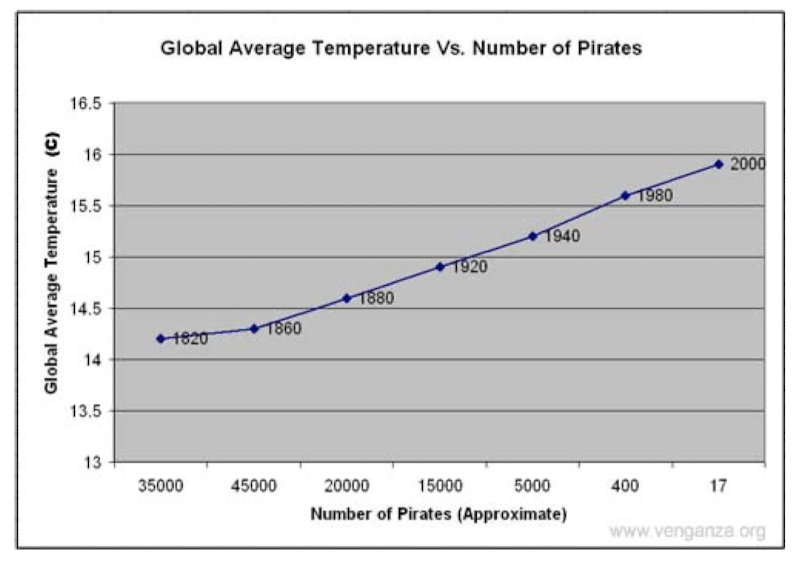
\includegraphics[width=\linewidth]{test_image}

\lipsum[1]

\noindent\dotfill

\lipsum[1]
% \sectiondivider

\end{multicols*}

\end{document}
